\documentclass{article}

\usepackage[utf8]{inputenc}
\usepackage{graphicx}
\usepackage{float}
\usepackage{tikz}
\usepackage{amsmath}
\usepackage{graphicx,lipsum,afterpage,subcaption}
\usepackage{enumitem}
\usepackage{svg}
\usepackage{amsmath}
\usepackage{longtable}
\usepackage{array}

\title{\textbf{Software Design Description}}

\begin{document}

\begin{figure}
    \centering
    
\includegraphics[height=5cm,width=5cm]{pitt-min.jpg}
\end{figure}

\author{Thomas Bui, Justin Carter, Patrick Flaherty, Wesley Miller Philip Seitz}

\date{}

\maketitle

\newenvironment{subs}
  {\adjustwidth{3em}{0pt}}
  {\endadjustwidth}

\pagebreak 

\tableofcontents
\newpage

\section{Introduction}
    
    \subsection{Purpose}
    The purpose of this document is to outline the design views and decisions in the development of the Train Control Signaling System software, including all relevant diagrams and descriptions to describe the architecture, layout, and dependencies of the system and its modules.
    
    \subsection{Scope}
    \paragraph{}
     The purpose of this project is to design and implement a new Centralized Traffic Control Center and Signaling System for Light Rail Transit system. The final system will be an executable that will demonstrate a fully operational control center, communications, train and track control system simulator for the transit system. This system would include a specification and implementation of a Centralized Traffic Control Center, a Track Controller, a Track Model, a Train Controller, and a Train Model. These modules would all be interface-able with a user. Above all, we hope to provide a comfortable user experience along with the best pricing available.
    
    \subsection{Definitions, Acronyms, Abbreviations}
    \paragraph{} The following are a list of terms, each followed by synonyms and abbreviations. A definition of each of the terms then follows:
    \begin{itemize}
        \item Train Control Signaling System - TCSS\index{TCSS}
            \begin{itemize}
            \item The Train Signaling System is the complete deliverable which this SRS \index{SRS} shall specify.
            \end{itemize}
        \item Centralized Traffic Control - CTC \index{CTC}
            \begin{itemize}
            \item The Central Office is one of the major modules of the TCSS\index{TCSS}. The CTC \index{CTC} is able to track the locations of the trains in the railway, as well as communicate to these trains important and vital information.
            \end{itemize}
        \item Operation Control Center - OCC
            \begin{itemize}
            \item See \emph{Centralized Traffic Control}
            \end{itemize}
        \item Central Office
            \begin{itemize}
            \item See \emph{Centralized Traffic Control}
            \end{itemize}

        \item Track Controller \index{Track Controller}
            \begin{itemize}
            \item This is a major module of the TCSS\index{TCSS}. The Track Controller \index{Track Controller} is responsible for sending important information to both the CTC \index{CTC} and the Train Controller \index{Train Controller} (Through the Track and Train Models\index{Train Model}). It also is responsible for controlling the state of the tracks, such as track switching and railway crossing. This runs a PLC \index{PLC} and is configurable on a per-Track Controller \index{Track Controller} basis.
            \end{itemize}
        \item Train Controller \index{Train Controller}
            \begin{itemize}
            \item This is a vital  \emph{(See Vital)} component of the TCSS\index{TCSS}. It is responsible for regulating the speed of the train. It is also responsible for controlling various other features of the Train Model\index{Train Model}. It is directly interface-able by the train driver, and will be capable of being controlled in both automatic and manual modes. 
            \end{itemize}
        \item Track Model \index{Track Model}
            \begin{itemize}
            \item This is a major component of the TCSS\index{TCSS}. It is a digital representation of the track with which the Train Model\index{Train Model} rides over, and the model which the Track Controller \index{Track Controller} is responsible for. This is configurable via a formatted csv file that will allow the user to simulate and control over any track diagram.
            \end{itemize}
        \item Train Model\index{Train Model}
            \begin{itemize}
            \item This is a major component of the TCSS\index{TCSS}. It is a digital representation of the Train with which the Train Controller \index{Train Controller} is responsible for. Furthermore it is a representation of the effect of Newtonian physics on the TCSS\index{TCSS} decision making.
            \end{itemize}
        \item Port Authority of Allegheny County - PAAC
            \begin{itemize}
            \item A public transit agency within Pennsylvania.
            \end{itemize}    
        \item Programmable Logic Controller - PLC \index{PLC}
            \begin{itemize}
            \item This is a logic controller that is specially programmable on a per-device basis. It is often adapted for the control of systems and devices that require a high reliability and ease of programming.
            \end{itemize}
        \item Vital
            \begin{itemize}
            \item Safety-Critical
            \end{itemize}
        \item Java Runtime Environment - JRE
            \begin{itemize}
            \item  The JRE is a virtual machine that enables a host computer to execute programs written in Java.
            \end{itemize}
        \item Office Open XML Workbook - XLSX
            \begin{itemize}
            \item  Office Open XML is a zipped, XML-based file format developed by Microsoft for representing spreadsheets, charts, presentations and word processing documents.
            \end{itemize}
        \item Graphic User Interface\index{interface} - GUI
            \begin{itemize}
                \item An electronic user interface \index{interface} displayed through a screen so that a user may interact with software.
            \end{itemize}
    \end{itemize}
    
    \subsection{References}
    \begin{itemize}
        \item Blackpool Flexity Tram Specifications, Bombardier Inc., 2009. Contained in professor-supplied Project Information directory.
    \end{itemize}
    \subsection{Overview}
    \paragraph{}
    The rest of the document outlines the basic design of the TCSS. In section 2, the system is outlined as a whole, dealing mostly with how outside actors, the users, will interact with the system. Section 3 looks at each module individually, relaying how they interact with each other as well as users.

\section{System Architecture}
    
    \subsection{System Architectural Design}
    \begin{figure}[H]
        \centering
        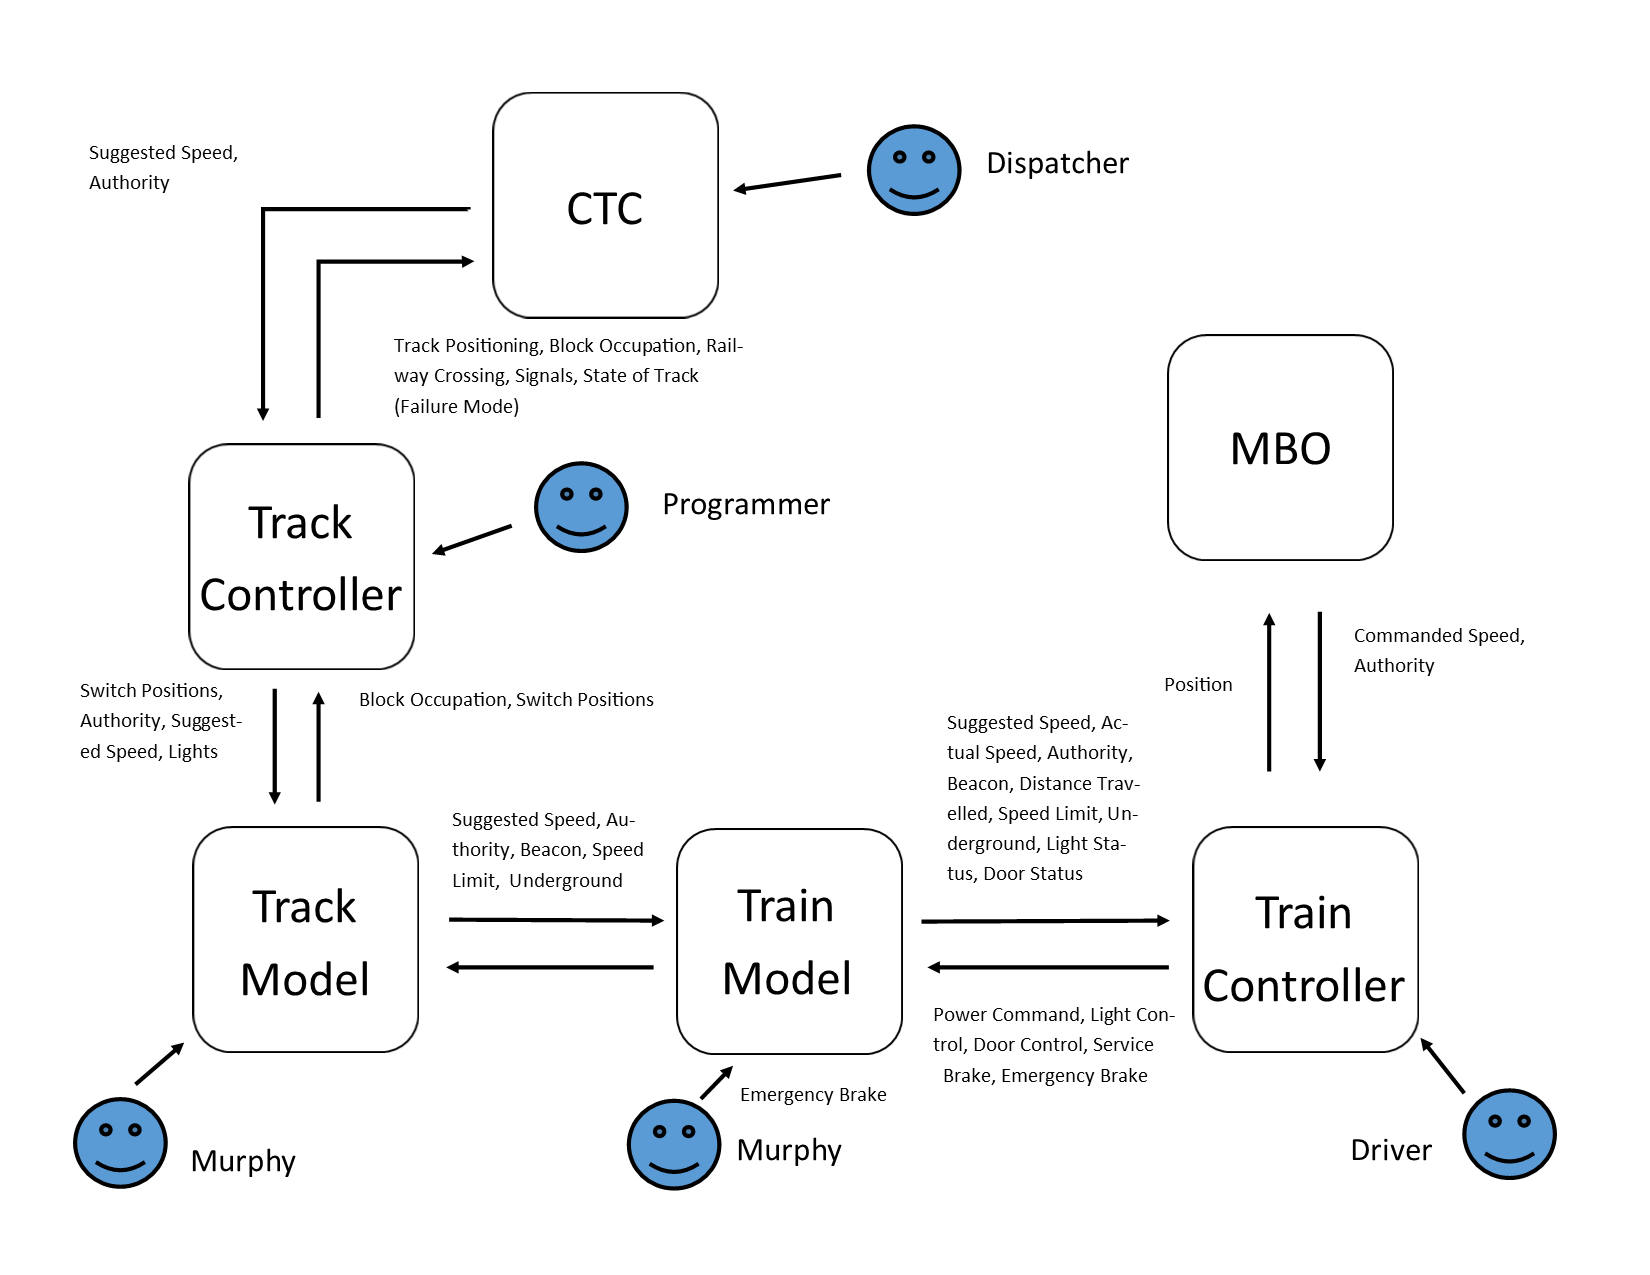
\includegraphics[width=\textwidth]{./System/Architecture Diagram.png}
        \caption{System Architecture}
        \label{fig:system_architecture}
    \end{figure}
    
    \subsection{System Design Description}
    
    \subsubsection{System Use Cases Diagram}
    \begin{figure}[H]
        \centering
        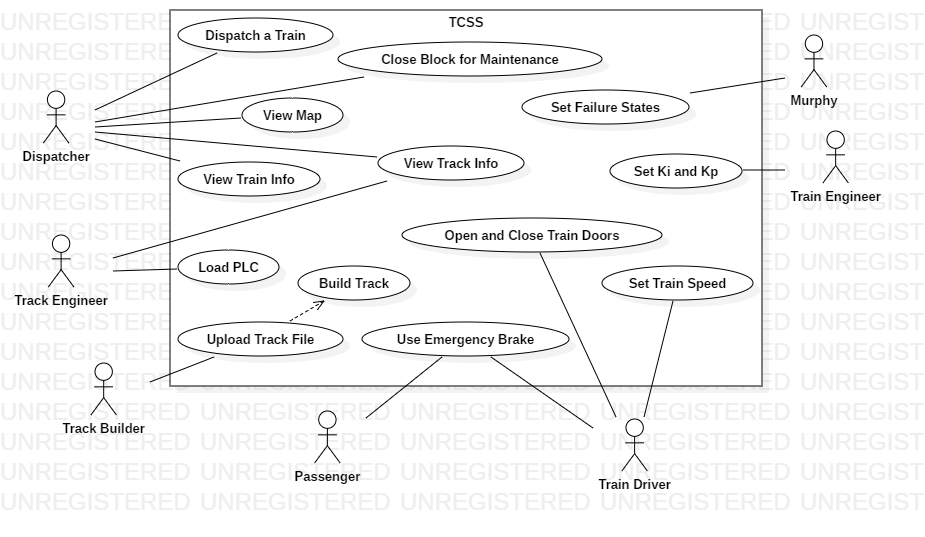
\includegraphics[width=\textwidth]{./System/System_UseCases.png}
        \caption{System Use Case Diagram}
        \label{fig:system_Use_Cases}
    \end{figure}
    
    \subsubsection{System Use Case Descriptions}
    \paragraph{}
   \begin{longtable}{
    || >{\raggedright\arraybackslash}m{0.15 \textwidth}
    | >{\raggedright\arraybackslash}m{0.85 \textwidth}||}
    \hline
    \textbf{System} & \textbf{System} \\
    \hline
    Use Case & Dispatcher dispatches a new train\\
    \hline
    Actors & CTC, Track Controller, Track Model, Train Model, Train Controller\\
    \hline
    Description & \begin{itemize}
        \item CTC receives new dispatch request
        \item CTC computes and sends new suggested speed and authority to the Track Controller at the calculated time
        \item Track Controller passes suggested speed and authority to designated block (start block)
        \item Track Model creates a train and adds it to the start block
        \item Train model sends speed and authority to Train Controller
    \end{itemize}\\
    \hline
    Data & Input: New dispatch request \newline Output: Train\\
    \hline
    Stimulus & Dispatcher wants to dispatch a new train\\
    \hline
    Response & Train is added to system at designated time and given suggested speed and authority\\
    \hline
    \end{longtable}
    \begin{longtable}{
    || >{\raggedright\arraybackslash}m{0.15 \textwidth}
    | >{\raggedright\arraybackslash}m{0.85 \textwidth}||}
    \hline
    \textbf{System} & \textbf{System} \\
    \hline
    Use Case & Dispatcher closes a new block for maintenance\\
    \hline
    Actors & CTC, Track Controller, Track Model\\
    \hline
    Description & \begin{itemize}
        \item CTC receives close block request
        \item CTC sends suggested speed and authority to Track Controller at designated time
        \item Track Controller sends suggested speed and authority to designated block
        \item Track Model designates block as closed
        \item CTC sends suggested speed and authority after designated time
        \item Track Controller sends suggested speed and authority to designated block
        \item Track Model designates block as open
    \end{itemize}\\
    \hline
    Data & Input: New maintenance request \newline Output: Display block changes\\
    \hline
    Stimulus & Track block needs maintenance\\
    \hline
    Response & Dispatcher enters maintenance request to the system\\
    \hline
    \end{longtable}
    
    \begin{longtable}{
    || >{\raggedright\arraybackslash}m{0.15 \textwidth}
    | >{\raggedright\arraybackslash}m{0.85 \textwidth}||}
    \hline
    \textbf{System} & \textbf{System} \\
    \hline
    Use Case & Train Driver sets Train Speed \\
    \hline
    Actors & Train Driver, Train Controller, Track Model, Train Model\\
    \hline
    Description & \begin{itemize}
        \item Train driver assigns a setpoint speed to the train controller in manual mode
        \item The suggested speed and authority of the train are transmitted to the train controller through the track circuit
        \item The train controller determines a safe operating speed by comparing the suggested speed, and setpoint speed, and considers both authority and system faults
        \item The train controller transmits a power command to the train model
        \item the speed of the train is adjusted according to the power command or brake command
        \item The displays of all the appropriate displays are updated to reflect the new operating conditions
    \end{itemize}\\
    \hline
    Data & Input: Set-point speed \newline Output: Train Speed Changes \\
    \hline
    Stimulus & Driver or Murphy enter a new setpoint speed\\
    \hline
    Response & The train model adjusts in speed and relevant displays update to present this change\\
    \hline
    \end{longtable}
    
    
    
    \begin{longtable}{
    || >{\raggedright\arraybackslash}m{0.15 \textwidth}
    | >{\raggedright\arraybackslash}m{0.85 \textwidth}||}
    \hline
    \textbf{System} & \textbf{Track Controller} \\
    \hline
    Use Case & Upload PLC\\
    \hline
    Actors & Track Engineer\\
    \hline
    Description & \begin{itemize}
        \item Track Engineer shall upload PLC to Track Controller and set new values. 
        \item Track Controller shall pass values to the Track Model to update. 
    \end{itemize}\\
    \hline
    Data & Input: Actor Input \newline Output: Switch, lights, and railroad crossing\\
    \hline
    Stimulus & Track Engineer input\\
    \hline
    Response & Track Controller values are updated as necessary\\
    \hline
    \end{longtable}
    
    \subsubsection{System Class Diagram}
    \begin{figure}[H]
        \centering
        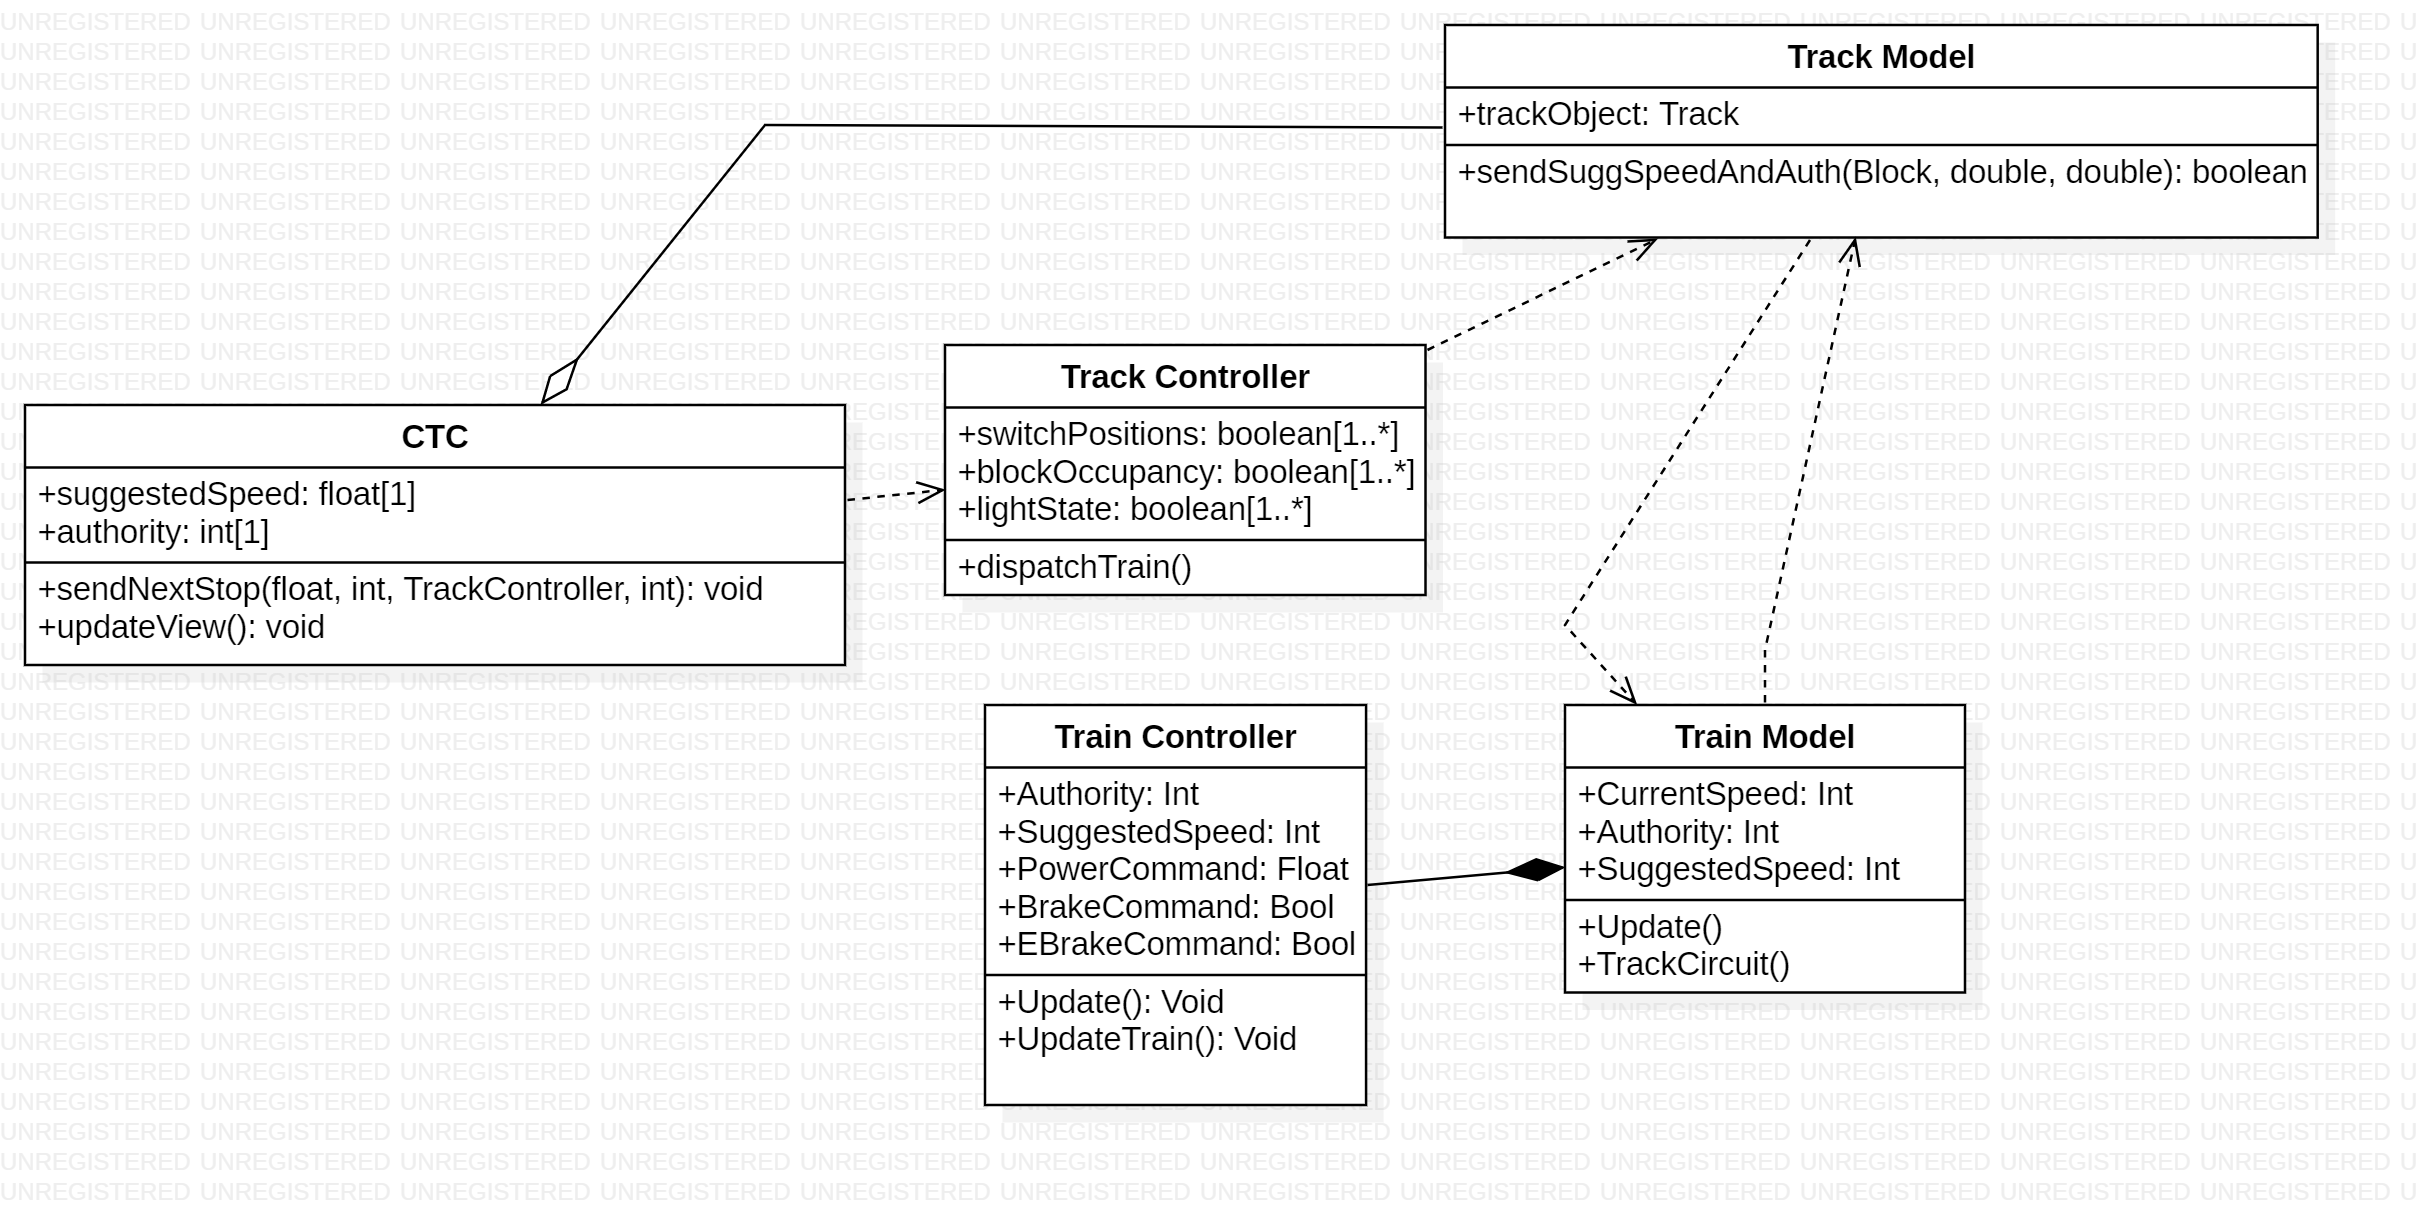
\includegraphics[width=\textwidth]{./System/System_Class_Diagram.png}
        \caption{System Class Diagram}
        \label{fig:System Class Diagram}
    \end{figure}
    \subsubsection{System Sequence Diagram}
    \begin{figure}[H]
        \centering
        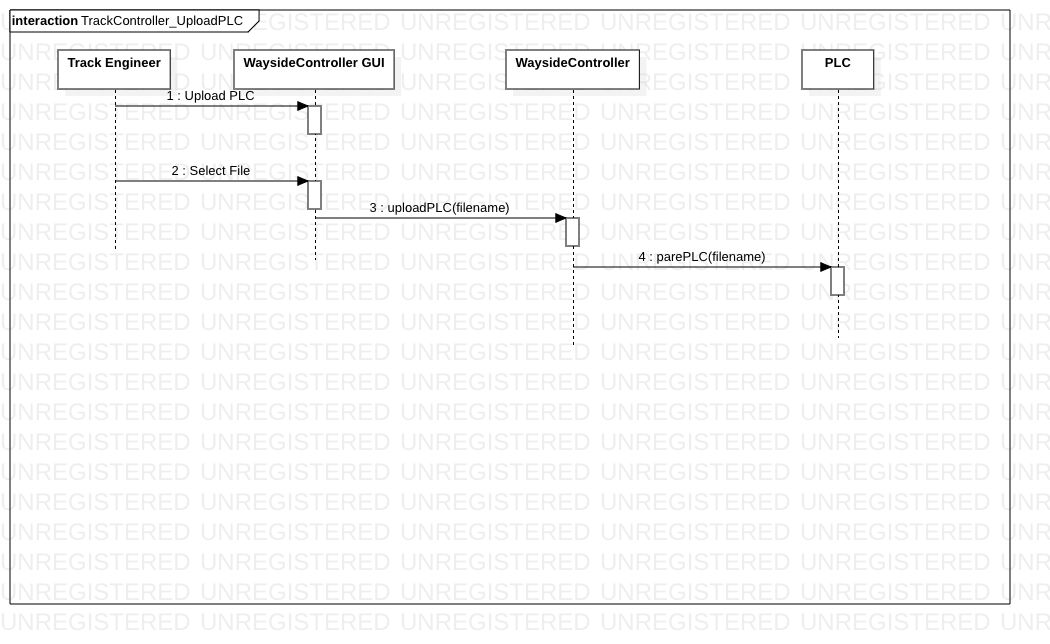
\includegraphics[width=\textwidth]{./SequenceDiagrams/TrackController_UploadPLC.png}
        \caption{Upload PLC System Sequence}
        \label{fig:Upload PLC System Sequence}
    \end{figure}
    \begin{figure}[H]
        \centering
        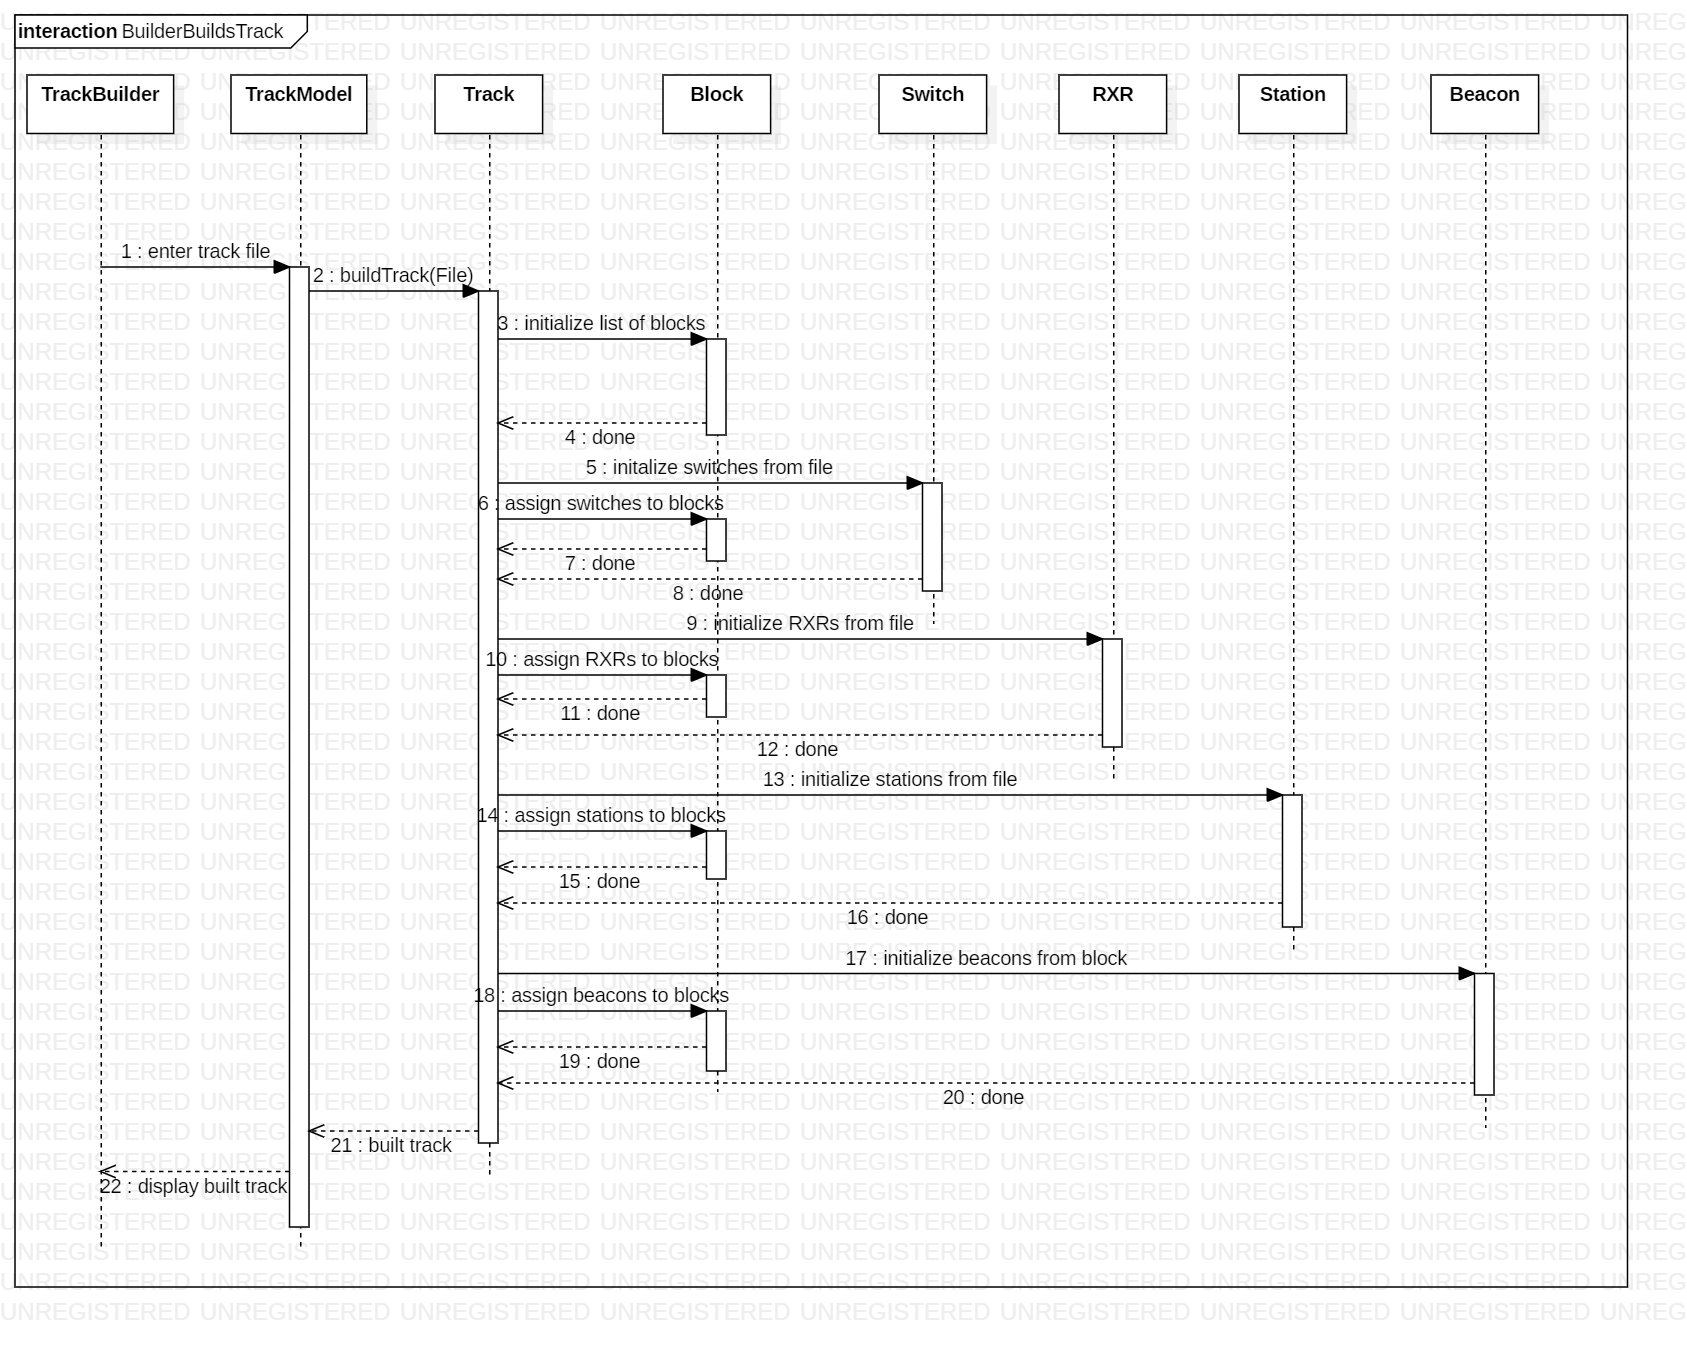
\includegraphics[width=\textwidth]{./SequenceDiagrams/TrackModel_SeqDiagrams/TrackModel_SeqDiagram_BuilderBuildsTrack.png}
        \caption{Use Case: Upload Track File System Sequence}
        \label{fig:Upload Track File System Sequence}
    \end{figure}
    
    \begin{figure}[H]
        \centering
        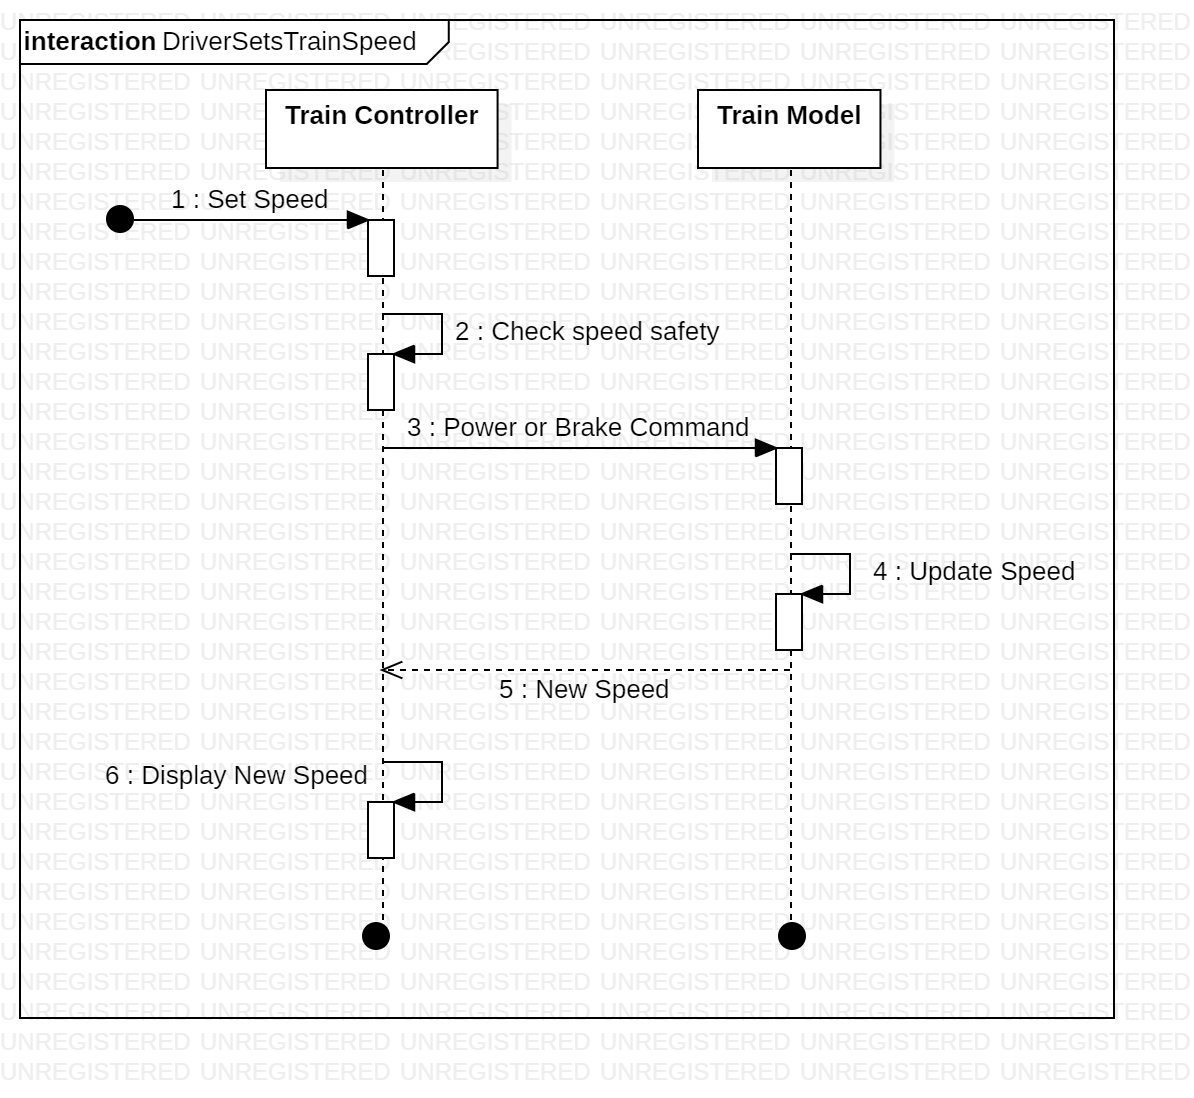
\includegraphics[width=\textwidth]{./System/Sequence/DriverTrainSpeed.png}
        \caption{Driver Sets Train Speed}
        \label{fig:d_train_speed_seq}
    \end{figure}
    
    \begin{figure}[H]
        \centering
        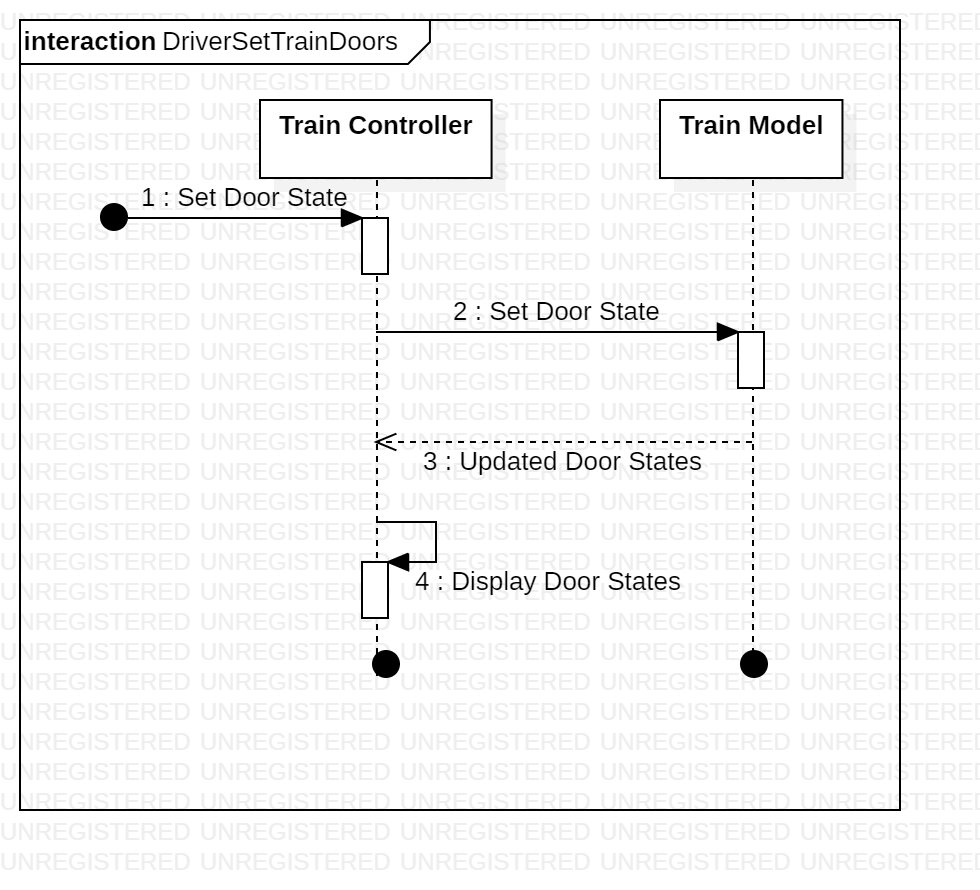
\includegraphics[width=\textwidth]{./System/Sequence/DriverDoors.png}
        \caption{Driver Sets Doors}
        \label{fig:d_door_seq}
    \end{figure}
    
    \begin{figure}[H]
        \centering
        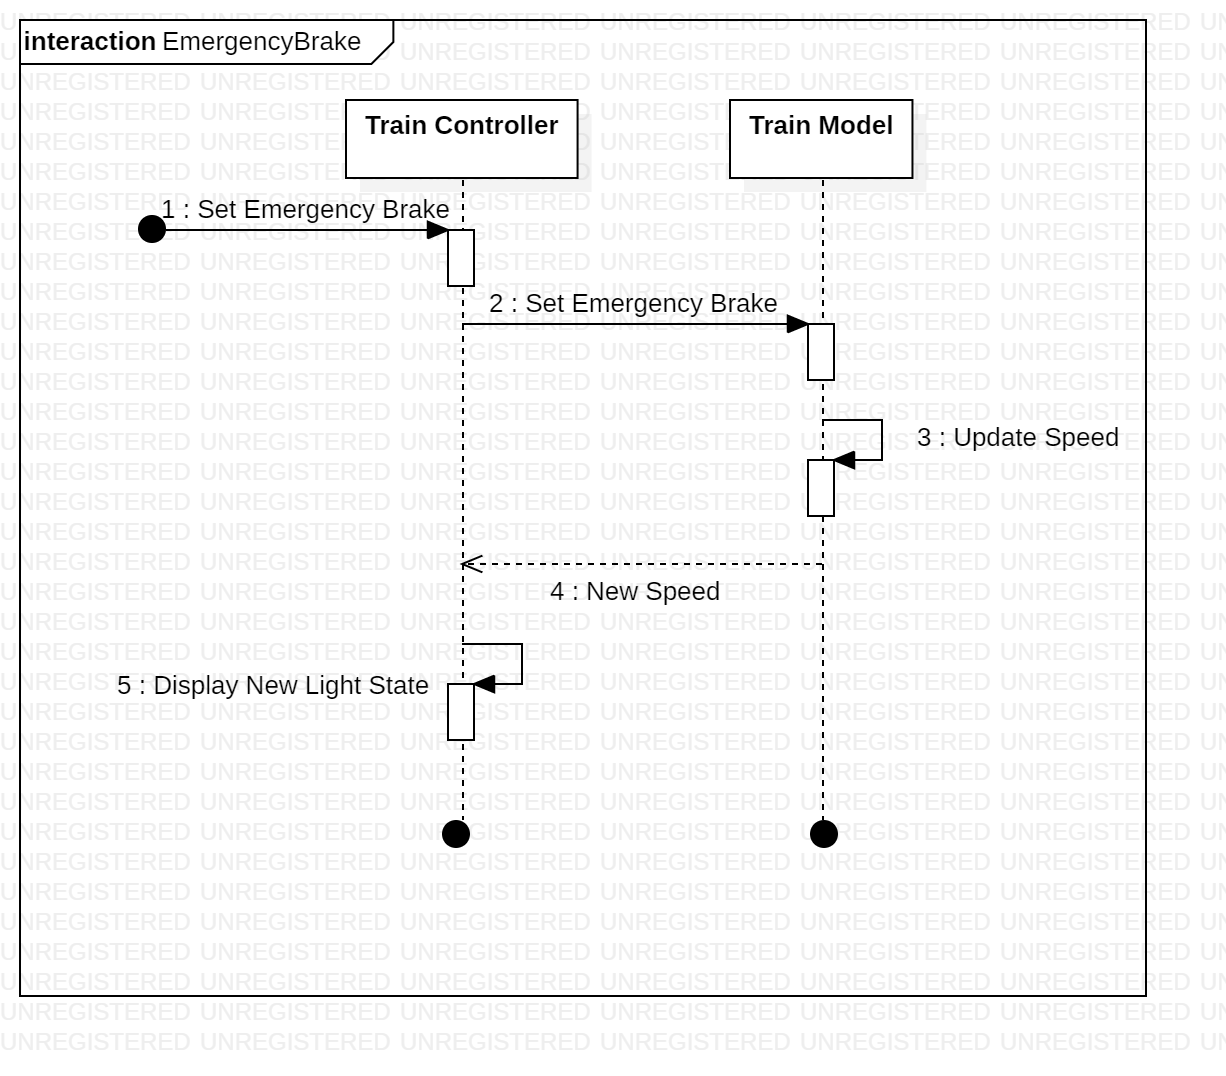
\includegraphics[width=\textwidth]{./System/Sequence/EBrake.png}
        \caption{User Sets Emergency Brake}
        \label{fig:system_ebrake_seq}
    \end{figure}
    
    \begin{figure}[H]
        \centering
        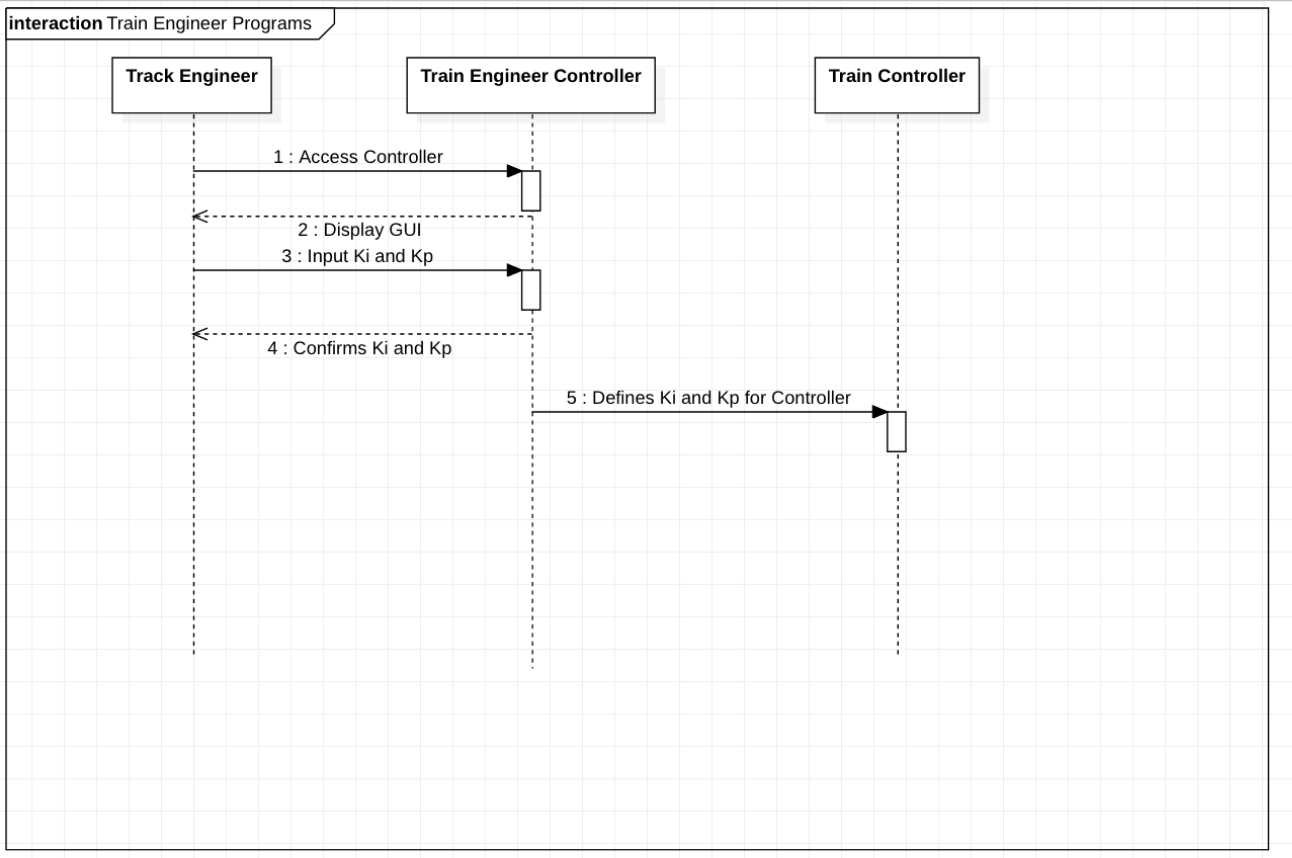
\includegraphics[width=\textwidth]{./TNCSD/TrainEngineerPrograms.png}
        \caption{Train Engineer Programs Ki and Kp}
        \label{fig:Train Engineer Programs Ki and Kp}
    \end{figure}
    
    \begin{figure}[H]
        \centering
        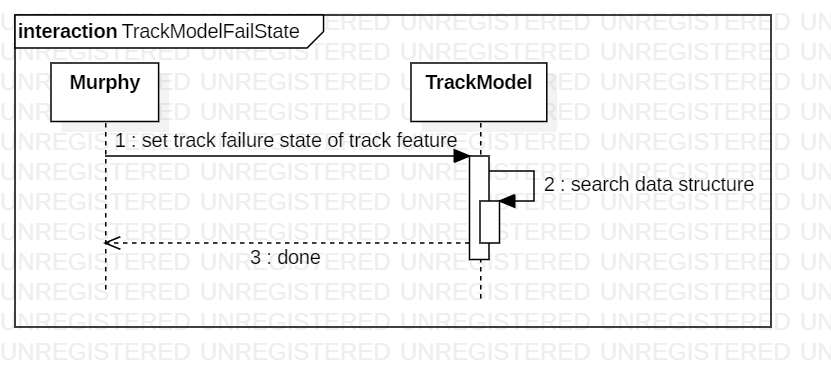
\includegraphics[width=\textwidth]{./System/Sequence/TrackModelFailState_SeqDiagram.png}
        \caption{Murphy Causes Track Failure}
        \label{fig:Murphy Causes Track Failure}
    \end{figure}
    
    \begin{figure}[H]
        \centering
        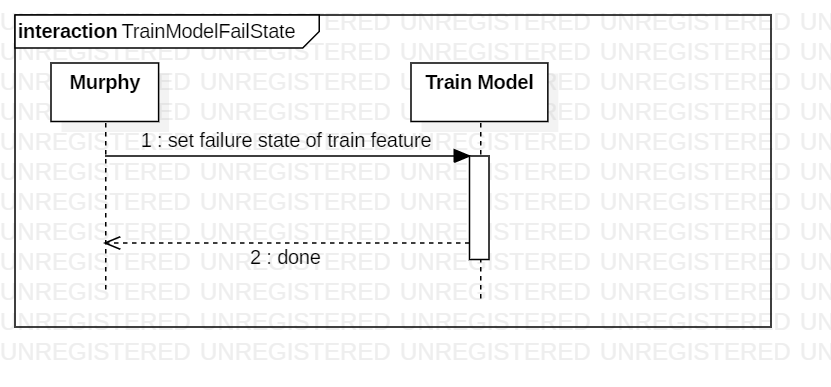
\includegraphics[width=\textwidth]{./System/Sequence/TrainModelFailState_SeqDiagram.png}
        \caption{Murphy Causes Train Failure}
        \label{fig:Murphy Causes Train Failure}
    \end{figure}
    
    \subsubsection{System Deployment Diagram}
    \begin{figure}[H]
        \centering
        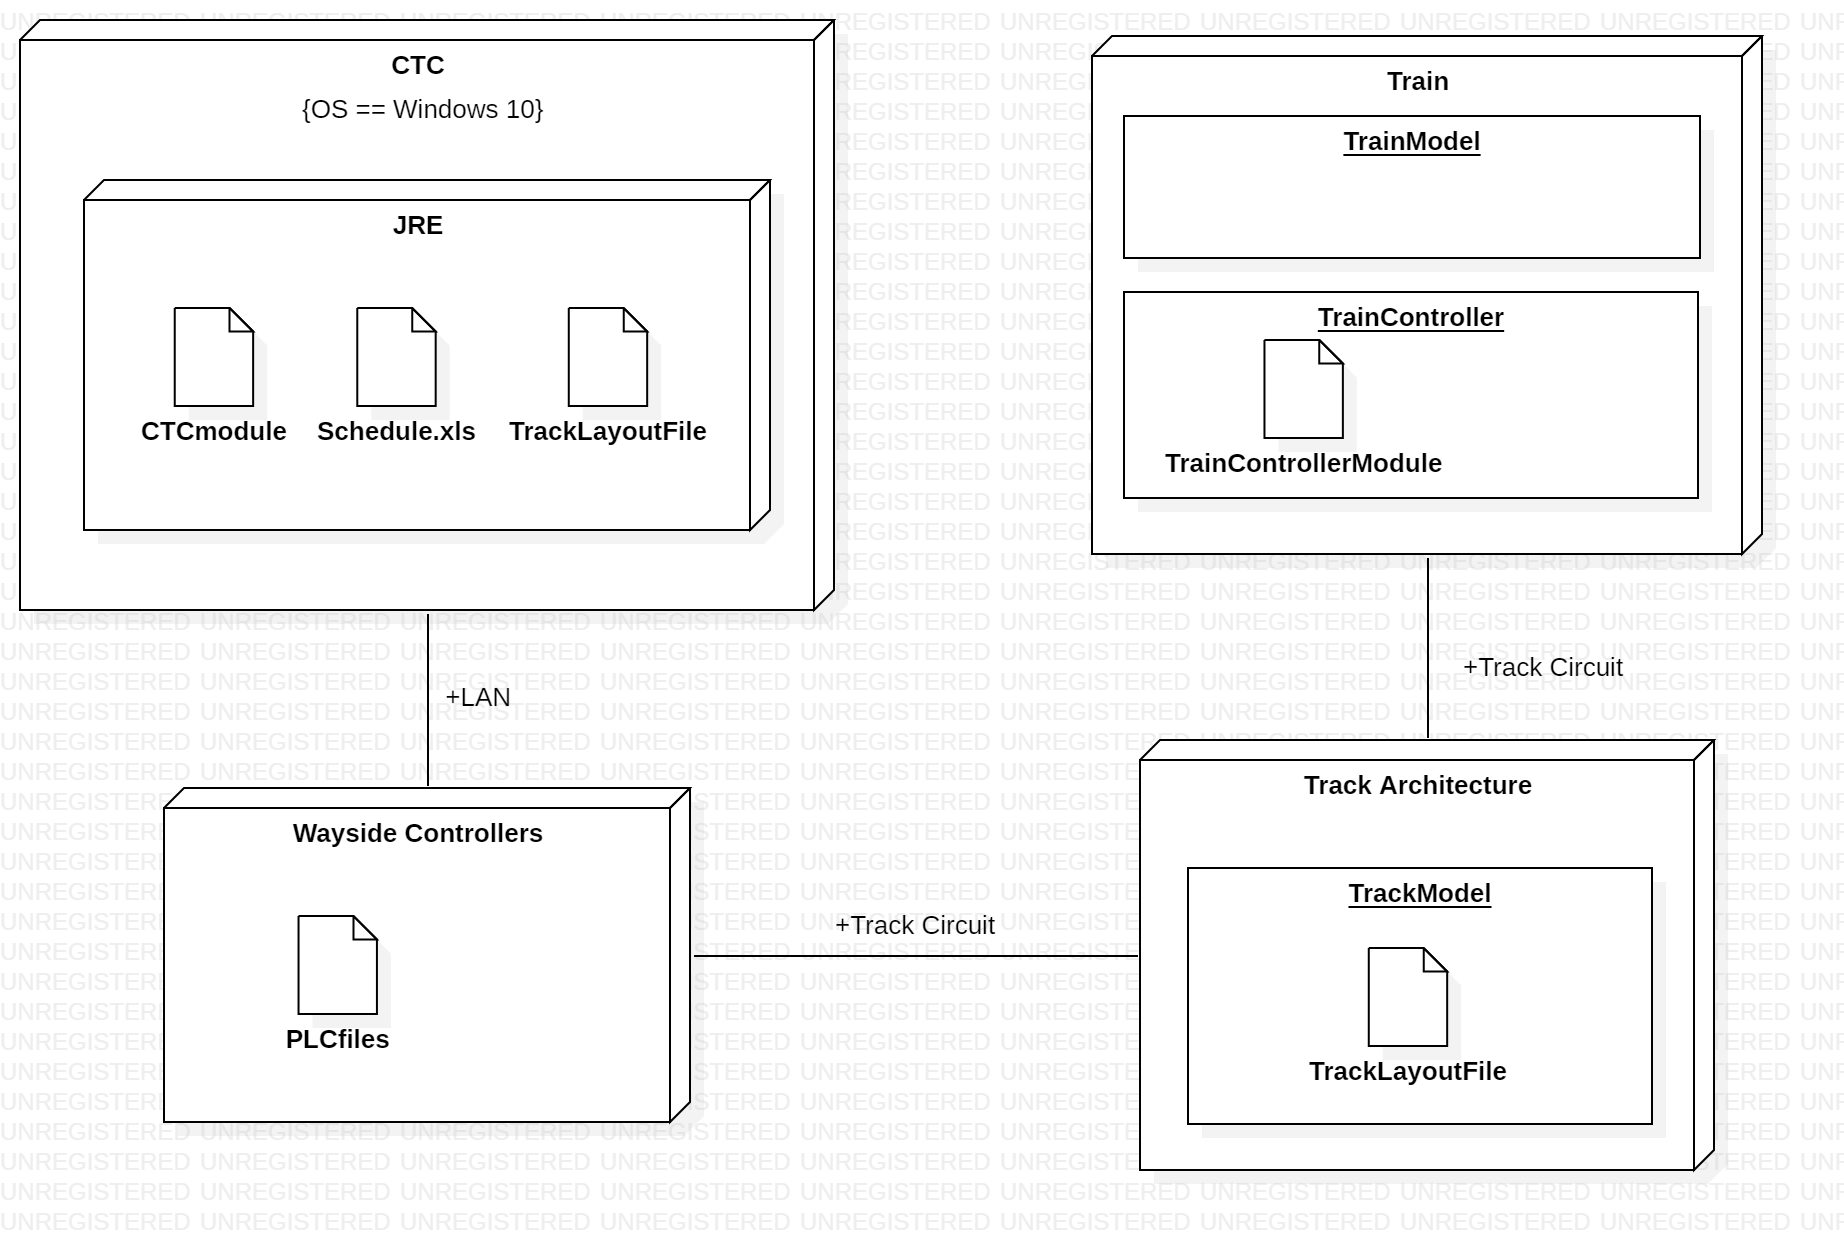
\includegraphics[width=\textwidth]{./System/DeploymentDiagram.png}
        \caption{System Deployment Diagram}
        \label{fig:deployment_diagram}
    \end{figure}


\section{Module Design}

    \subsection{Centralized Traffic Control}
    
    \subsubsection{Use Case Diagram}
     \begin{figure}[H]
        \centering
        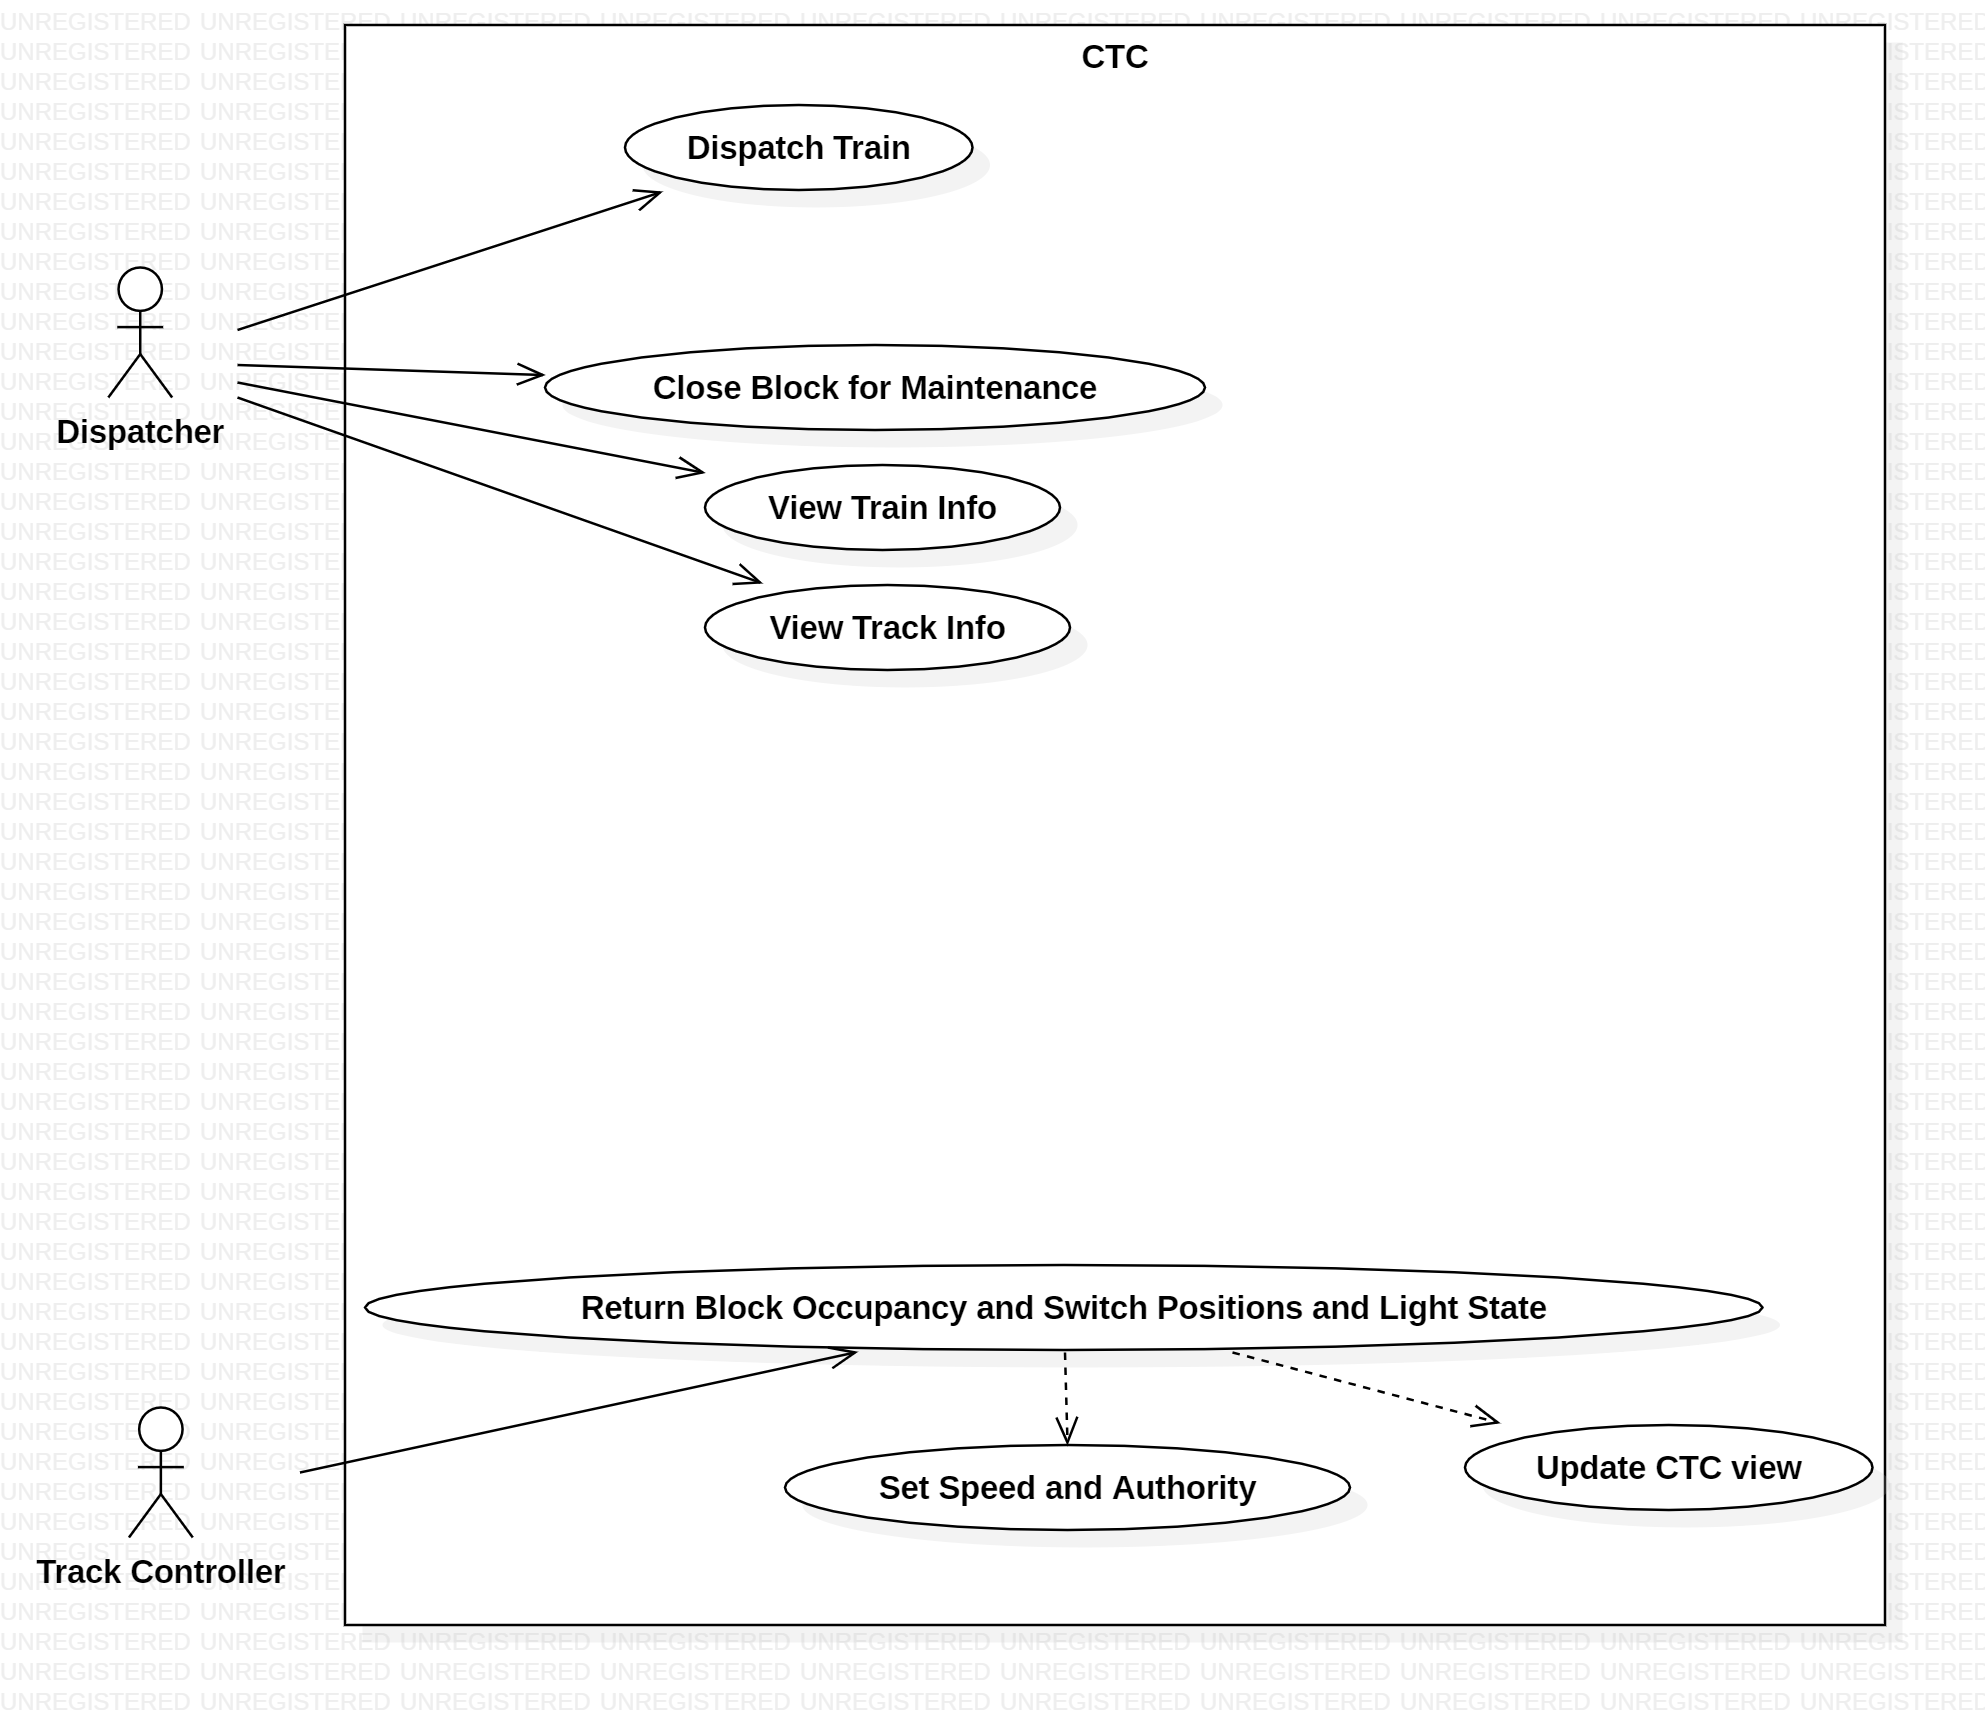
\includegraphics[width=\textwidth]{./CTC/CTC_UseCaseDiagram.png}
        \caption{CTC Use Cases}
        \label{fig: CTC Use Cases}
    \end{figure}
    \subsubsection{Use Case Descriptions}
    \paragraph{}
   \begin{longtable}{
    || >{\raggedright\arraybackslash}m{0.15 \textwidth}
    | >{\raggedright\arraybackslash}m{0.85 \textwidth}||}
    \hline
    \textbf{System} & \textbf{CTC} \\
    \hline
    Use Case & Dispatcher closes a block for maintenance\\
    \hline
    Actors & Dispatcher\\
    \hline
    Description & \begin{itemize}
        \item Dispatcher selects a track section from the CTC view
        \item Track Controller shall pass values to the Track Model to update. 
        \item Dispatcher selects a specific block from the section list
        \item Dispatcher sets start time and duration for maintenance and creates request
        \item Block is closed at time request is created
        \item Maintenance period starts at request start time
        \item Block is reopened after maintenance request is completed
    \end{itemize}\\
    \hline
    Data & Input: Actor Input \newline Output: Switch, lights, and railroad crossing\\
    \hline
    Stimulus & Dispatcher wants to close a block for maintenance\\
    \hline
    Response & The selected block is closed and re-opened when determined by the dispatcher\\
    \hline
    \end{longtable}
    \begin{longtable}{
    || >{\raggedright\arraybackslash}m{0.15 \textwidth}
    | >{\raggedright\arraybackslash}m{0.85 \textwidth}||}
    \hline
    \textbf{System} & \textbf{CTC} \\
    \hline
    Use Case & Dispatch a train\\
    \hline
    Actors & Dispatcher\\
    \hline
    Description & \begin{itemize}
        \item Dispatcher clicks on create new dispatch button
        \item Dispatcher selects dispatch mode
        \item Dispatcher selects schedule dependent on mode selected
        \item Dispatcher confirms dispatch
        \item New suggested speed and authority sent to the starting block at calculated start time of the dispatch

    \end{itemize}\\
    \hline
    Data & Input: Schedule, Dispatch \newline Output: Suggested Speed, Authority\\
    \hline
    Stimulus & New train needs to be dispatched in the system\\
    \hline
    Response & Dispatcher creates dispatch request and submits it to the system\\
    \hline
    \end{longtable}
    \begin{longtable}{
    || >{\raggedright\arraybackslash}m{0.15 \textwidth}
    | >{\raggedright\arraybackslash}m{0.85 \textwidth}||}
    \hline
    \textbf{System} & \textbf{CTC} \\
    \hline
    Use Case & View train information\\
    \hline
    Actors & Dispatcher\\
    \hline
    Description & \begin{itemize}
        \item Dispatcher clicks on an active dispatch from the CTC view
        \item Dispatcher clicks on train name from the dispatch selected
        \item Train information appears in the bottom of the screen
    \end{itemize}\\
    \hline
    Data & Input: Train name \newline Output: Formatted train information\\
    \hline
    Stimulus & Dispatcher wants to access current train information\\
    \hline
    Response & Formatted train information is displayed on the screen\\
    \hline
    \end{longtable}
    \begin{longtable}{
    || >{\raggedright\arraybackslash}m{0.15 \textwidth}
    | >{\raggedright\arraybackslash}m{0.85 \textwidth}||}
    \hline
    \textbf{System} & \textbf{CTC} \\
    \hline
    Use Case & View Track Information\\
    \hline
    Actors & Dispatcher\\
    \hline
    Description & \begin{itemize}
        \item Dispatcher selects a track section from the CTC view
        \item Dispatcher selects a specific block from the section list
        \item Block information is displayed onto the CTC view
    \end{itemize}\\
    \hline
    Data & Input: blockID \newline Output: Formatted block information\\
    \hline
    Stimulus & Dispatcher wants to access current status of a block\\
    \hline
    Response & Formatted block information is displayed on the screen\\
    \hline
    \end{longtable}
    \begin{longtable}{
    || >{\raggedright\arraybackslash}m{0.15 \textwidth}
    | >{\raggedright\arraybackslash}m{0.85 \textwidth}||}
    \hline
    \textbf{System} & \textbf{CTC} \\
    \hline
    Use Case & Set Speed and Authority\\
    \hline
    Actors & Dispatcher, Track Controller\\
    \hline
    Description & \begin{itemize}
        \item Track controller returns information to CTC (Block occupancy, switch positions, and light state)
        \item CTC updates track model representation inside module to reflect current track conditions
        \item CTC checks current train conditions for a need to send an updated speed and authority to a new block
        \item CTC sends a new speed and authority to the correct block for the desired train
    \end{itemize}\\
    \hline
    Data & Input: Block occupancy, switch positions, light state \newline Output: suggested speed, authority\\
    \hline
    Stimulus & Global update to send information back to CTC to update information\\
    \hline
    Response & Dispatch list checked and new suggested speed and authorities sent as needed\\
    \hline
    \end{longtable}
    \begin{longtable}{
    || >{\raggedright\arraybackslash}m{0.15 \textwidth}
    | >{\raggedright\arraybackslash}m{0.85 \textwidth}||}
    \hline
    \textbf{System} & \textbf{CTC} \\
    \hline
    Use Case & Update CTC view\\
    \hline
    Actors & Dispatcher, Track Controller\\
    \hline
    Description & \begin{itemize}
        \item Track controller returns information to CTC (Block occupancy, switch positions, and light state)
        \item CTC updates track model representation inside module to reflect current track conditions
        \item CTC map view is updated accordingly
    \end{itemize}\\
    \hline
    Data & Input: Block occupancy, switch positions, and light state \newline Output: formatted track model view in GUI\\
    \hline
    Stimulus & Global update to send information back to CTC to update information\\
    \hline
    Response & Track model view in GUI is updated on the screen\\
    \hline
    \end{longtable}
    \subsubsection{Class Diagrams}
    \begin{figure}[H]
        \centering
        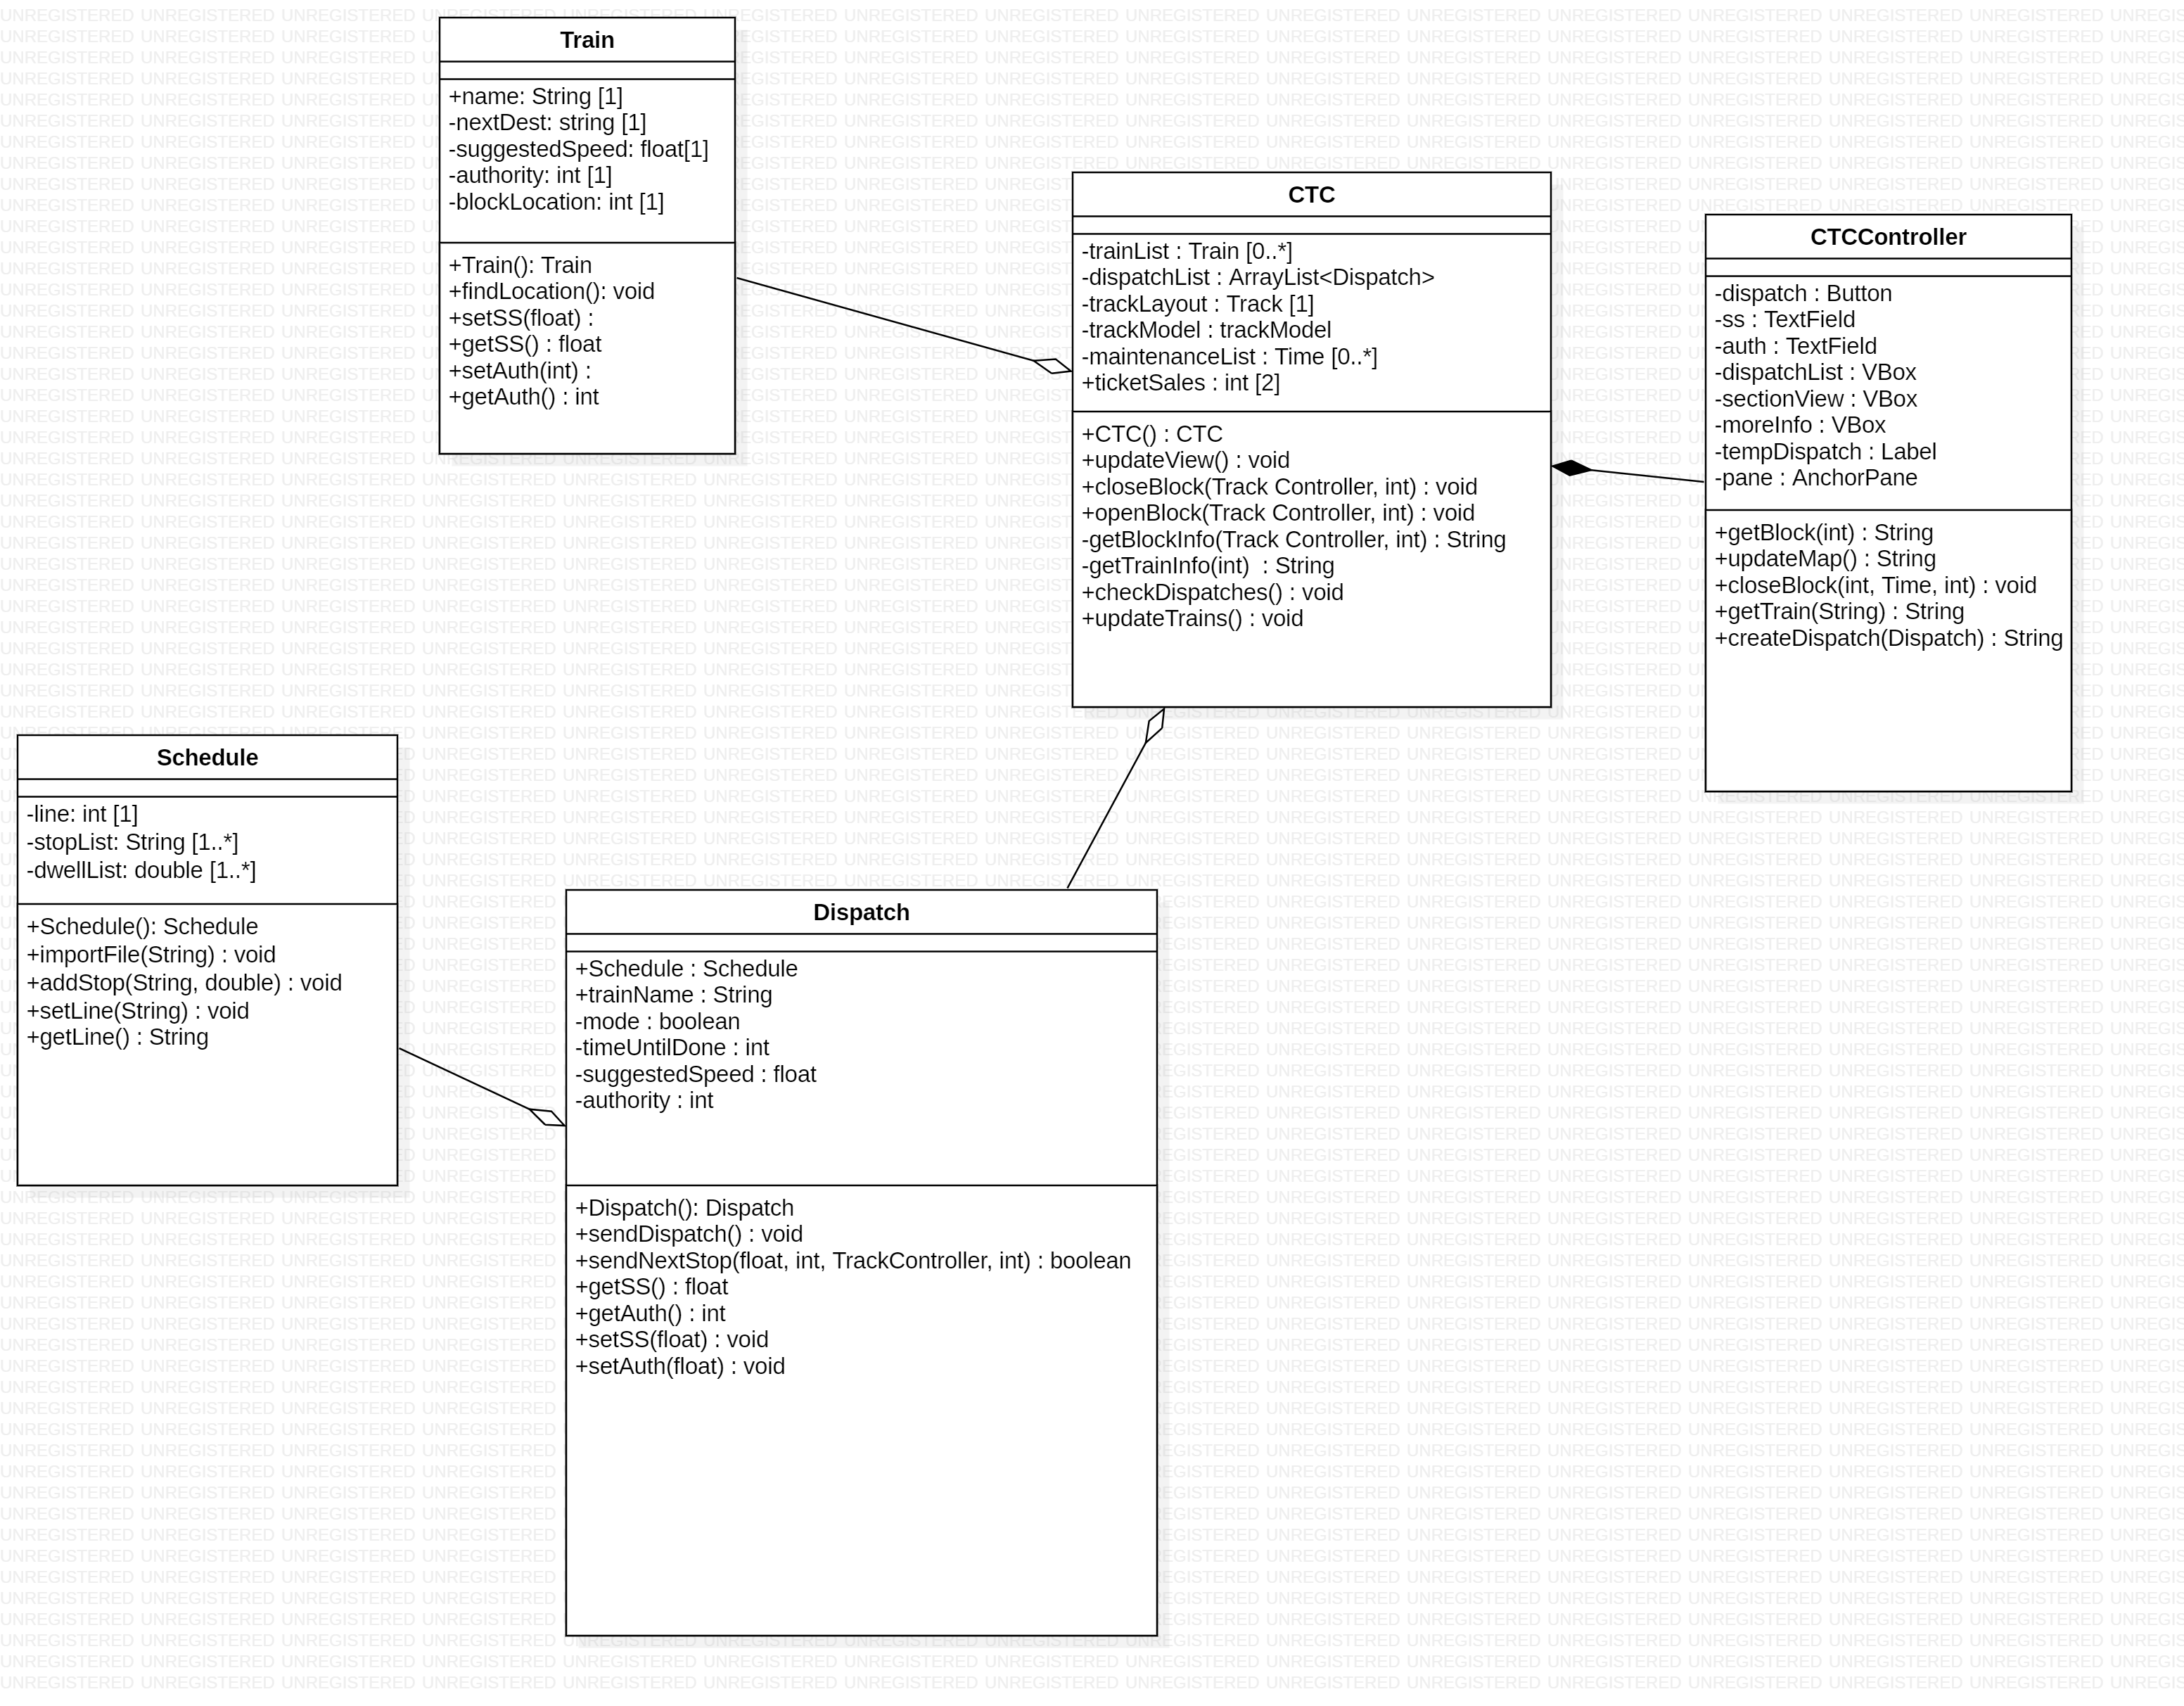
\includegraphics[width=\textwidth]{./CTC/CTC_Class_Diagram.png}
        \caption{CTC Class Diagram}
        \label{fig:CTC Class Diagram}
    \end{figure}
    \subsubsection{Sequence Diagrams}
    \begin{figure}[H]
        \centering
        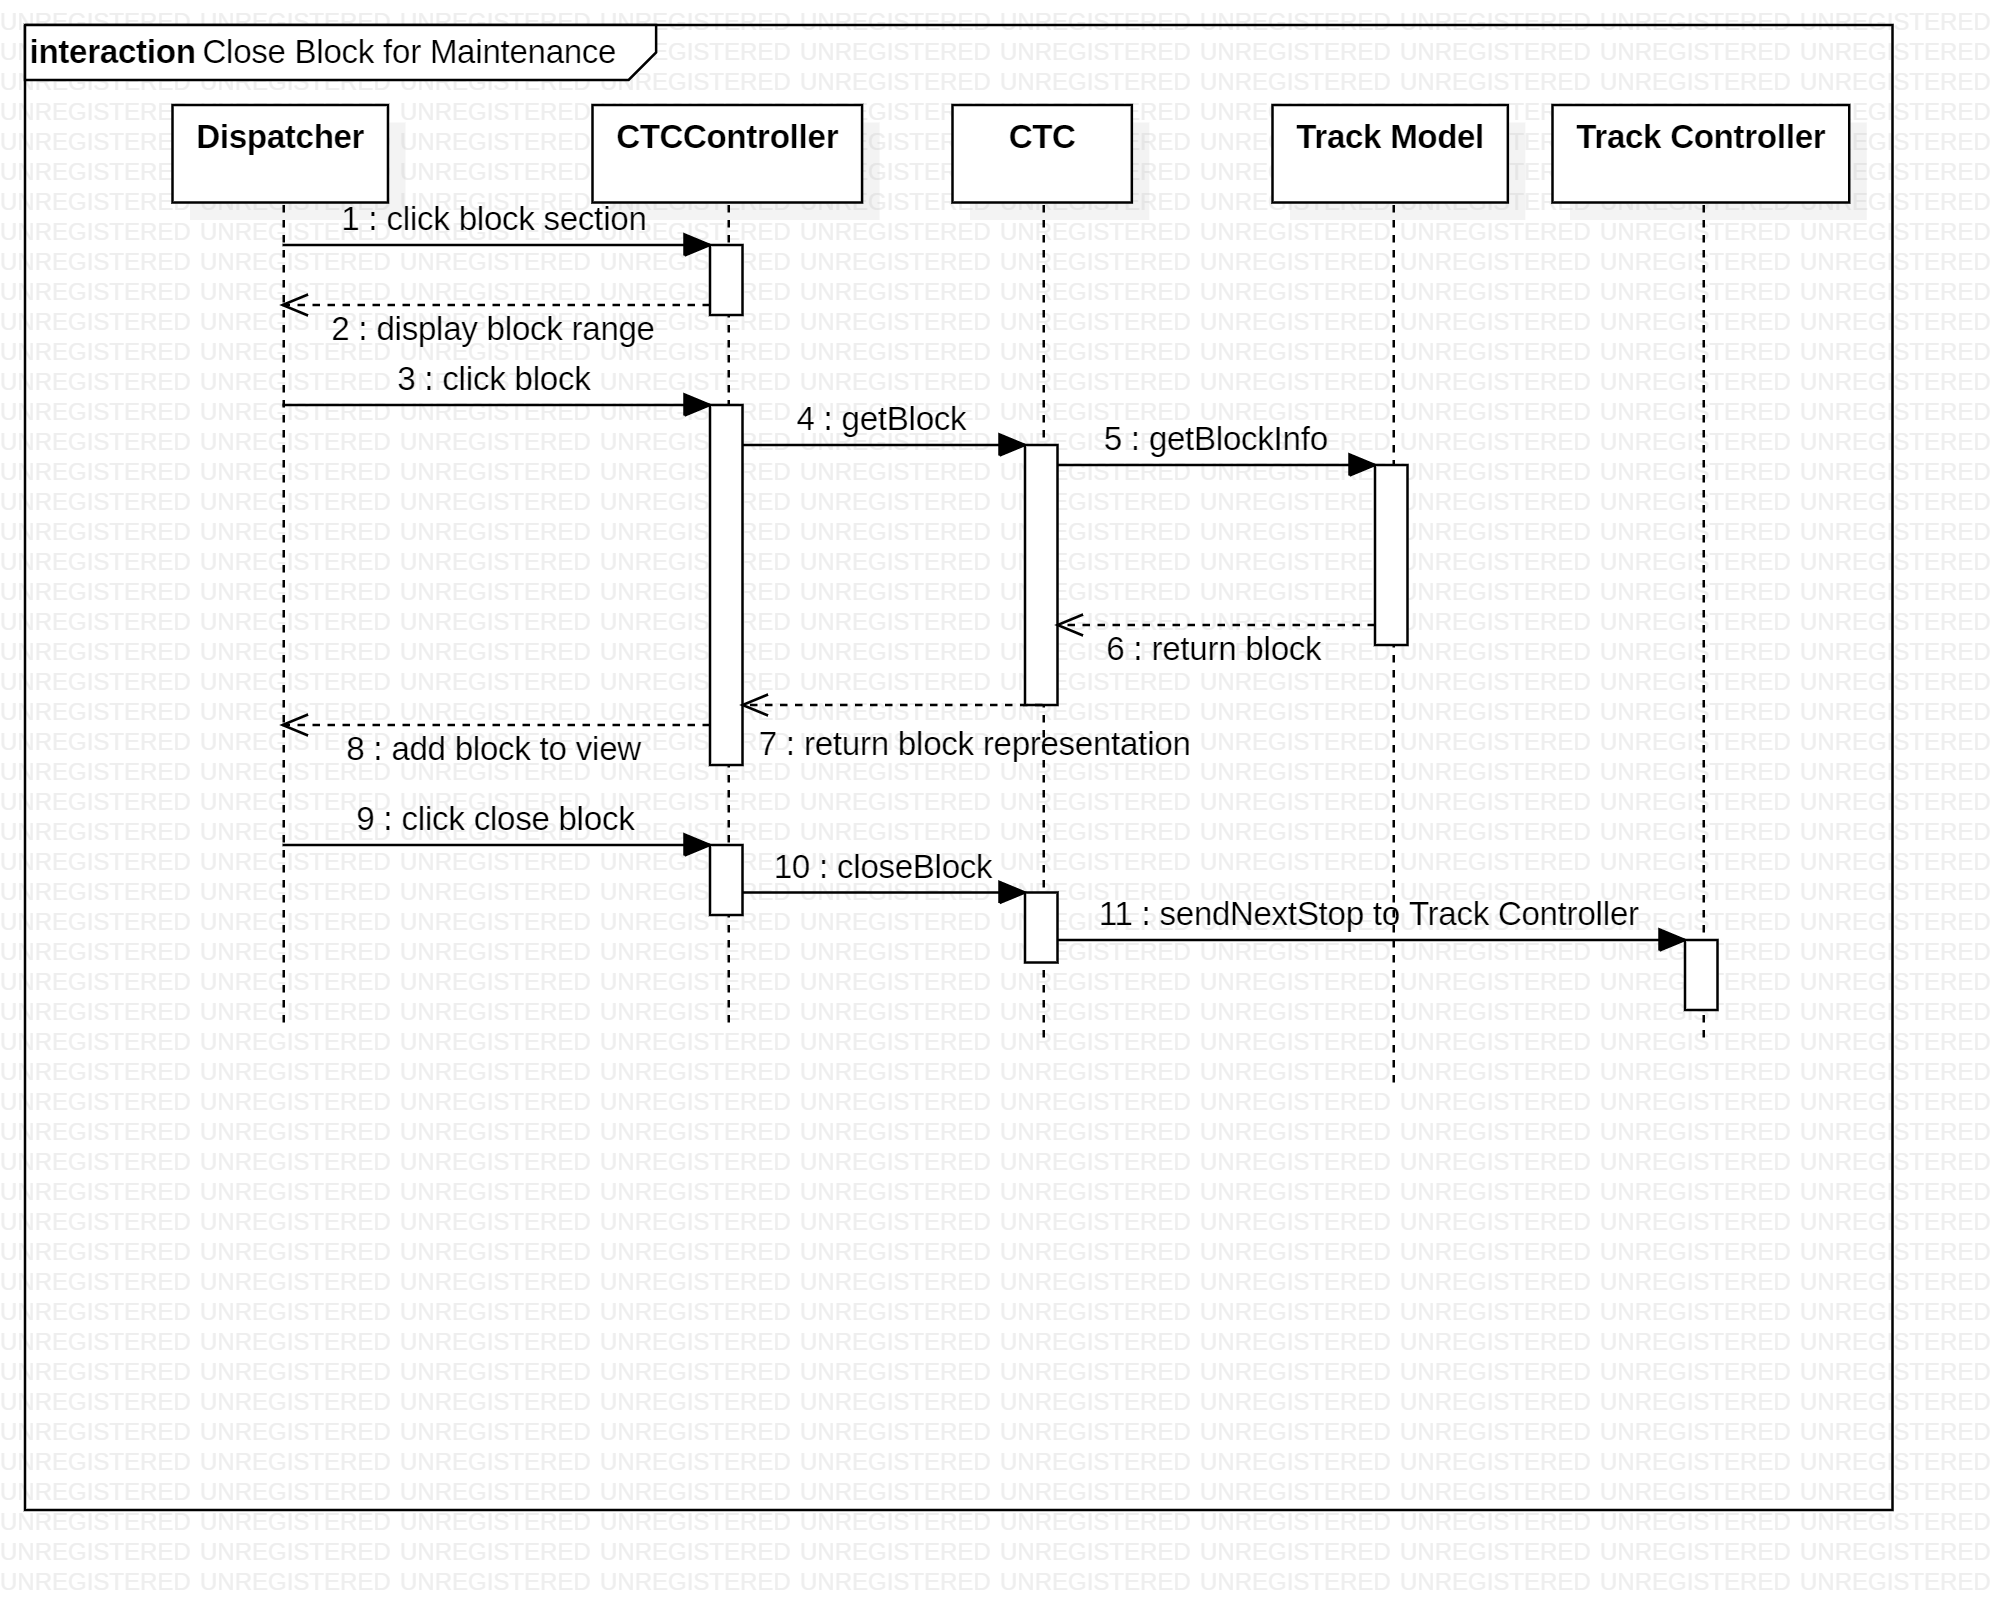
\includegraphics[width=\textwidth]{./CTC/Close_Block_for_Maintenance.png}
        \caption{CTC Close Block for Maintenance}
        \label{fig:Use Case: CTC Closes Block for Maintenance}
    \end{figure}
     \begin{figure}[H]
        \centering
        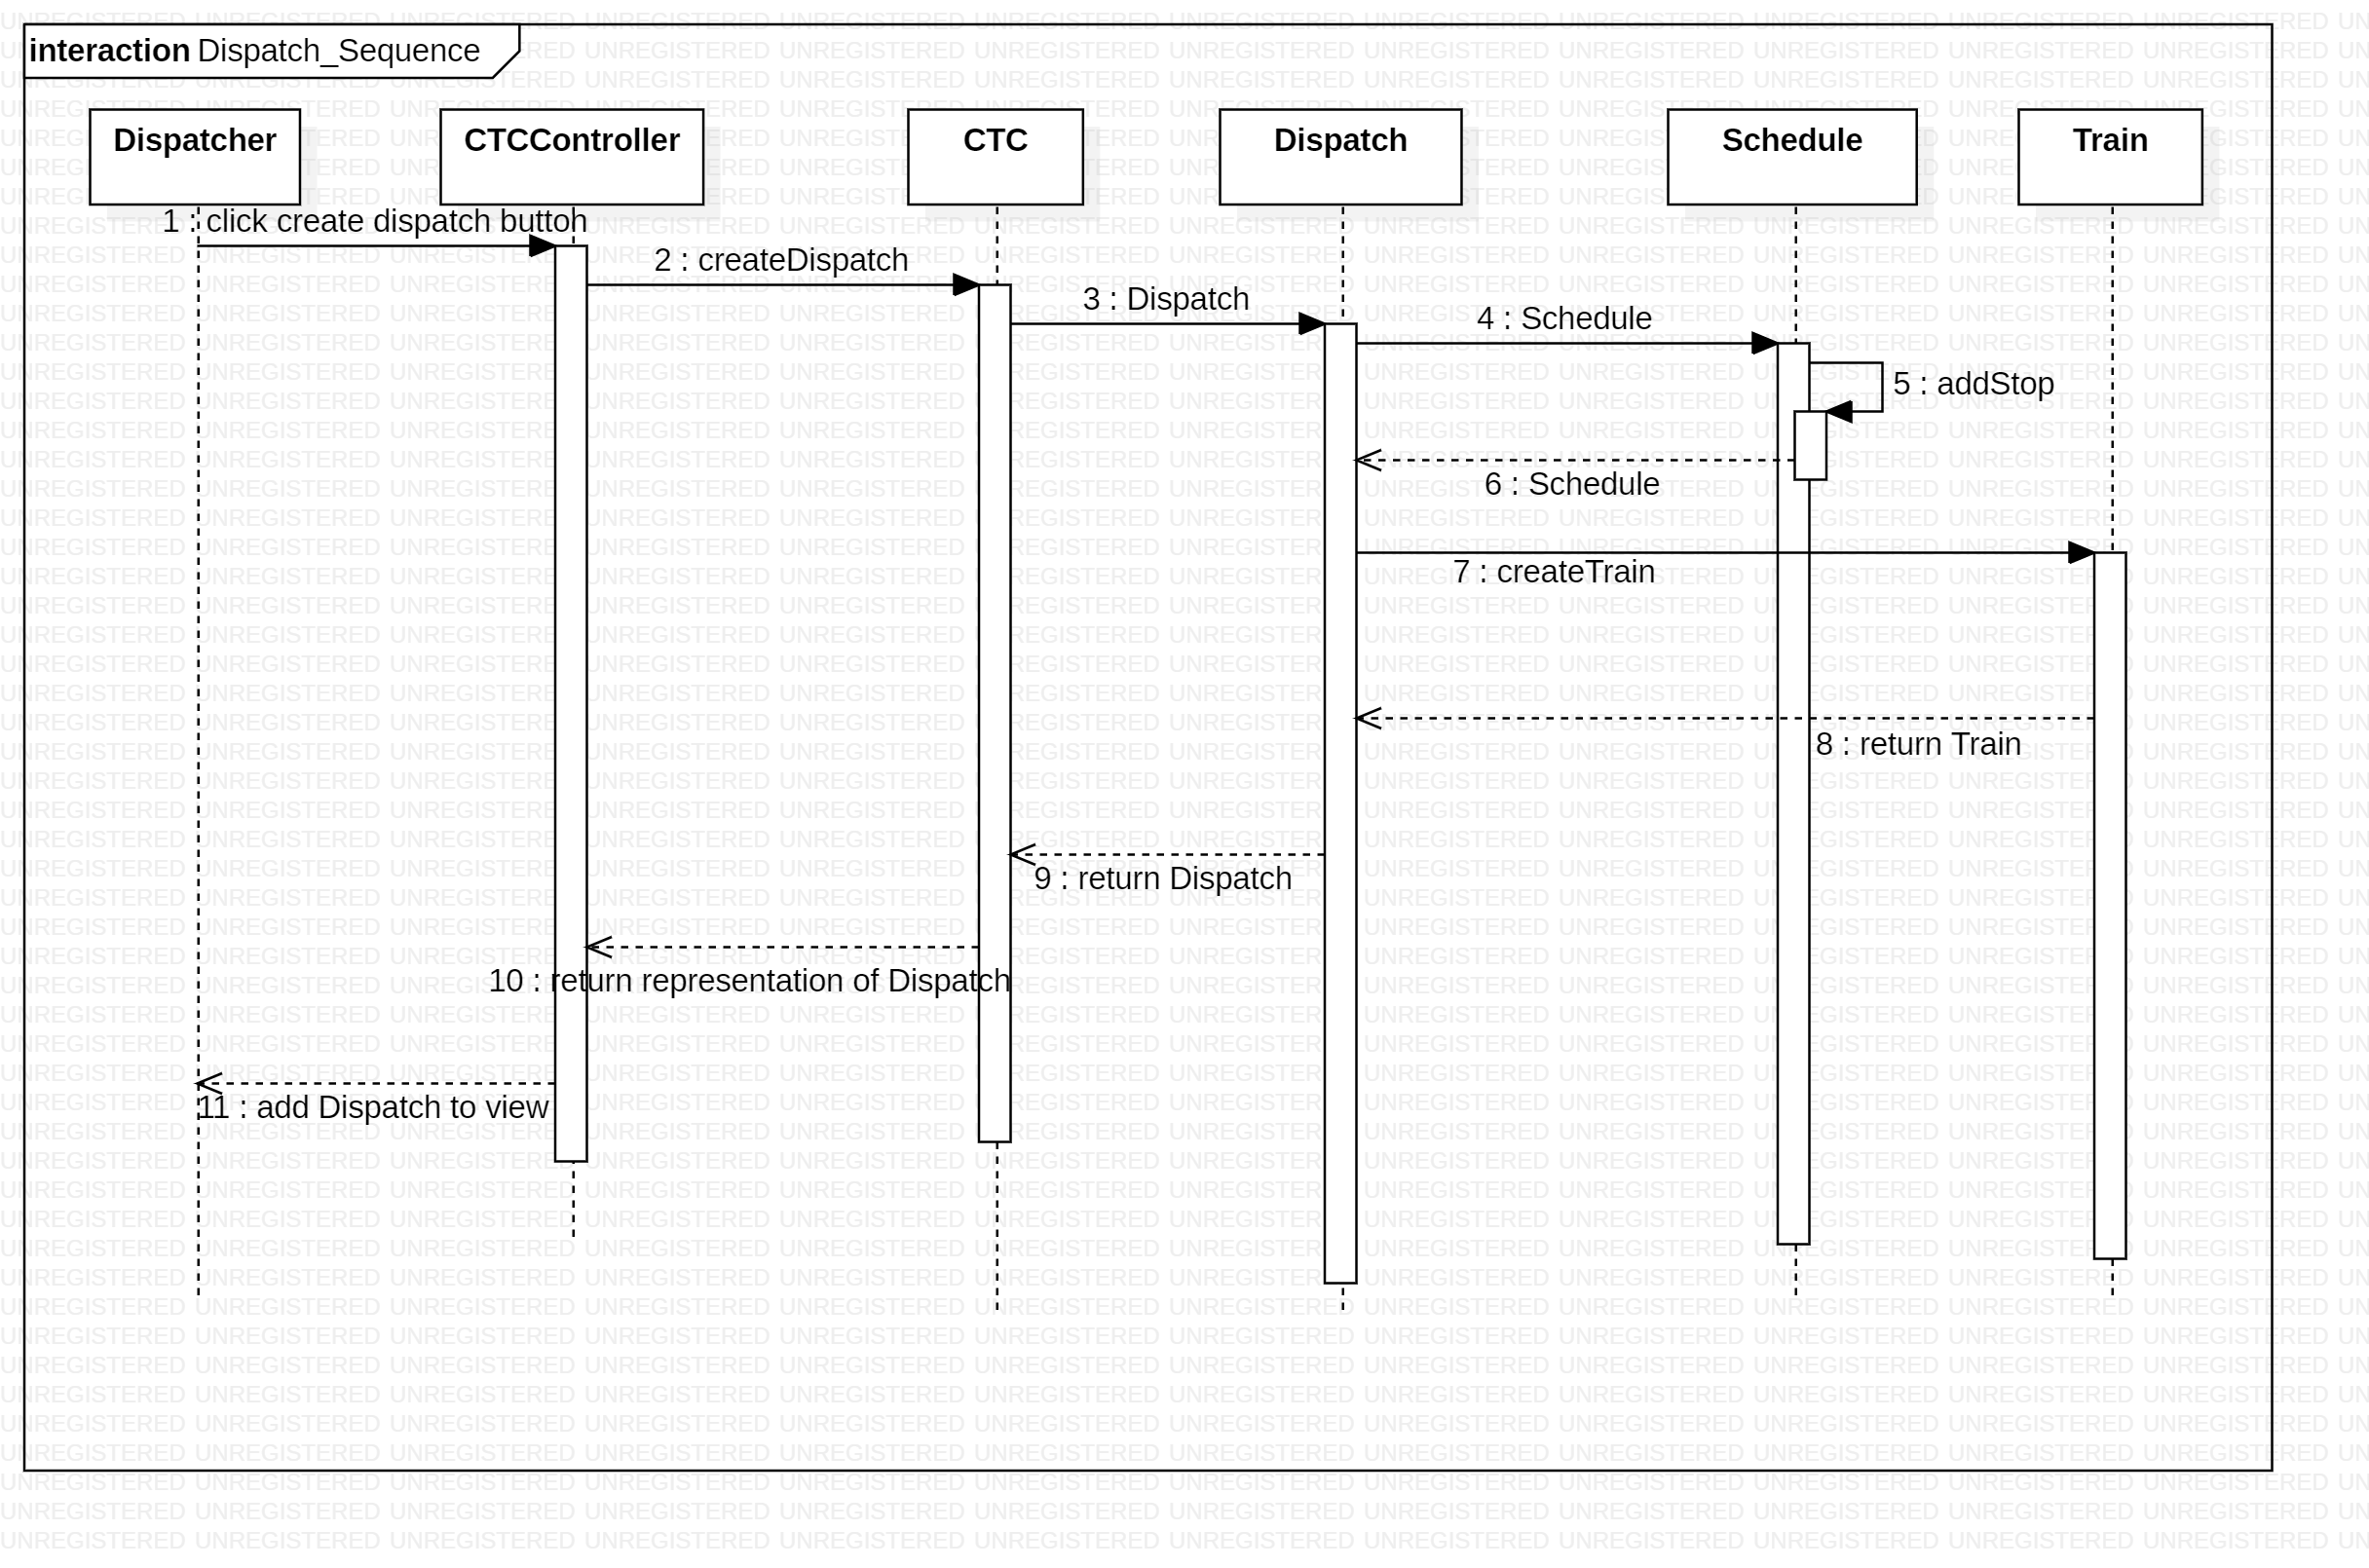
\includegraphics[width=\textwidth]{./CTC/Dispatch_Sequence.png}
        \caption{Dispatcher Dispatches a new train}
        \label{fig:Use Case: Dispatcher dispatches a new train}
    \end{figure}
     \begin{figure}[H]
        \centering
        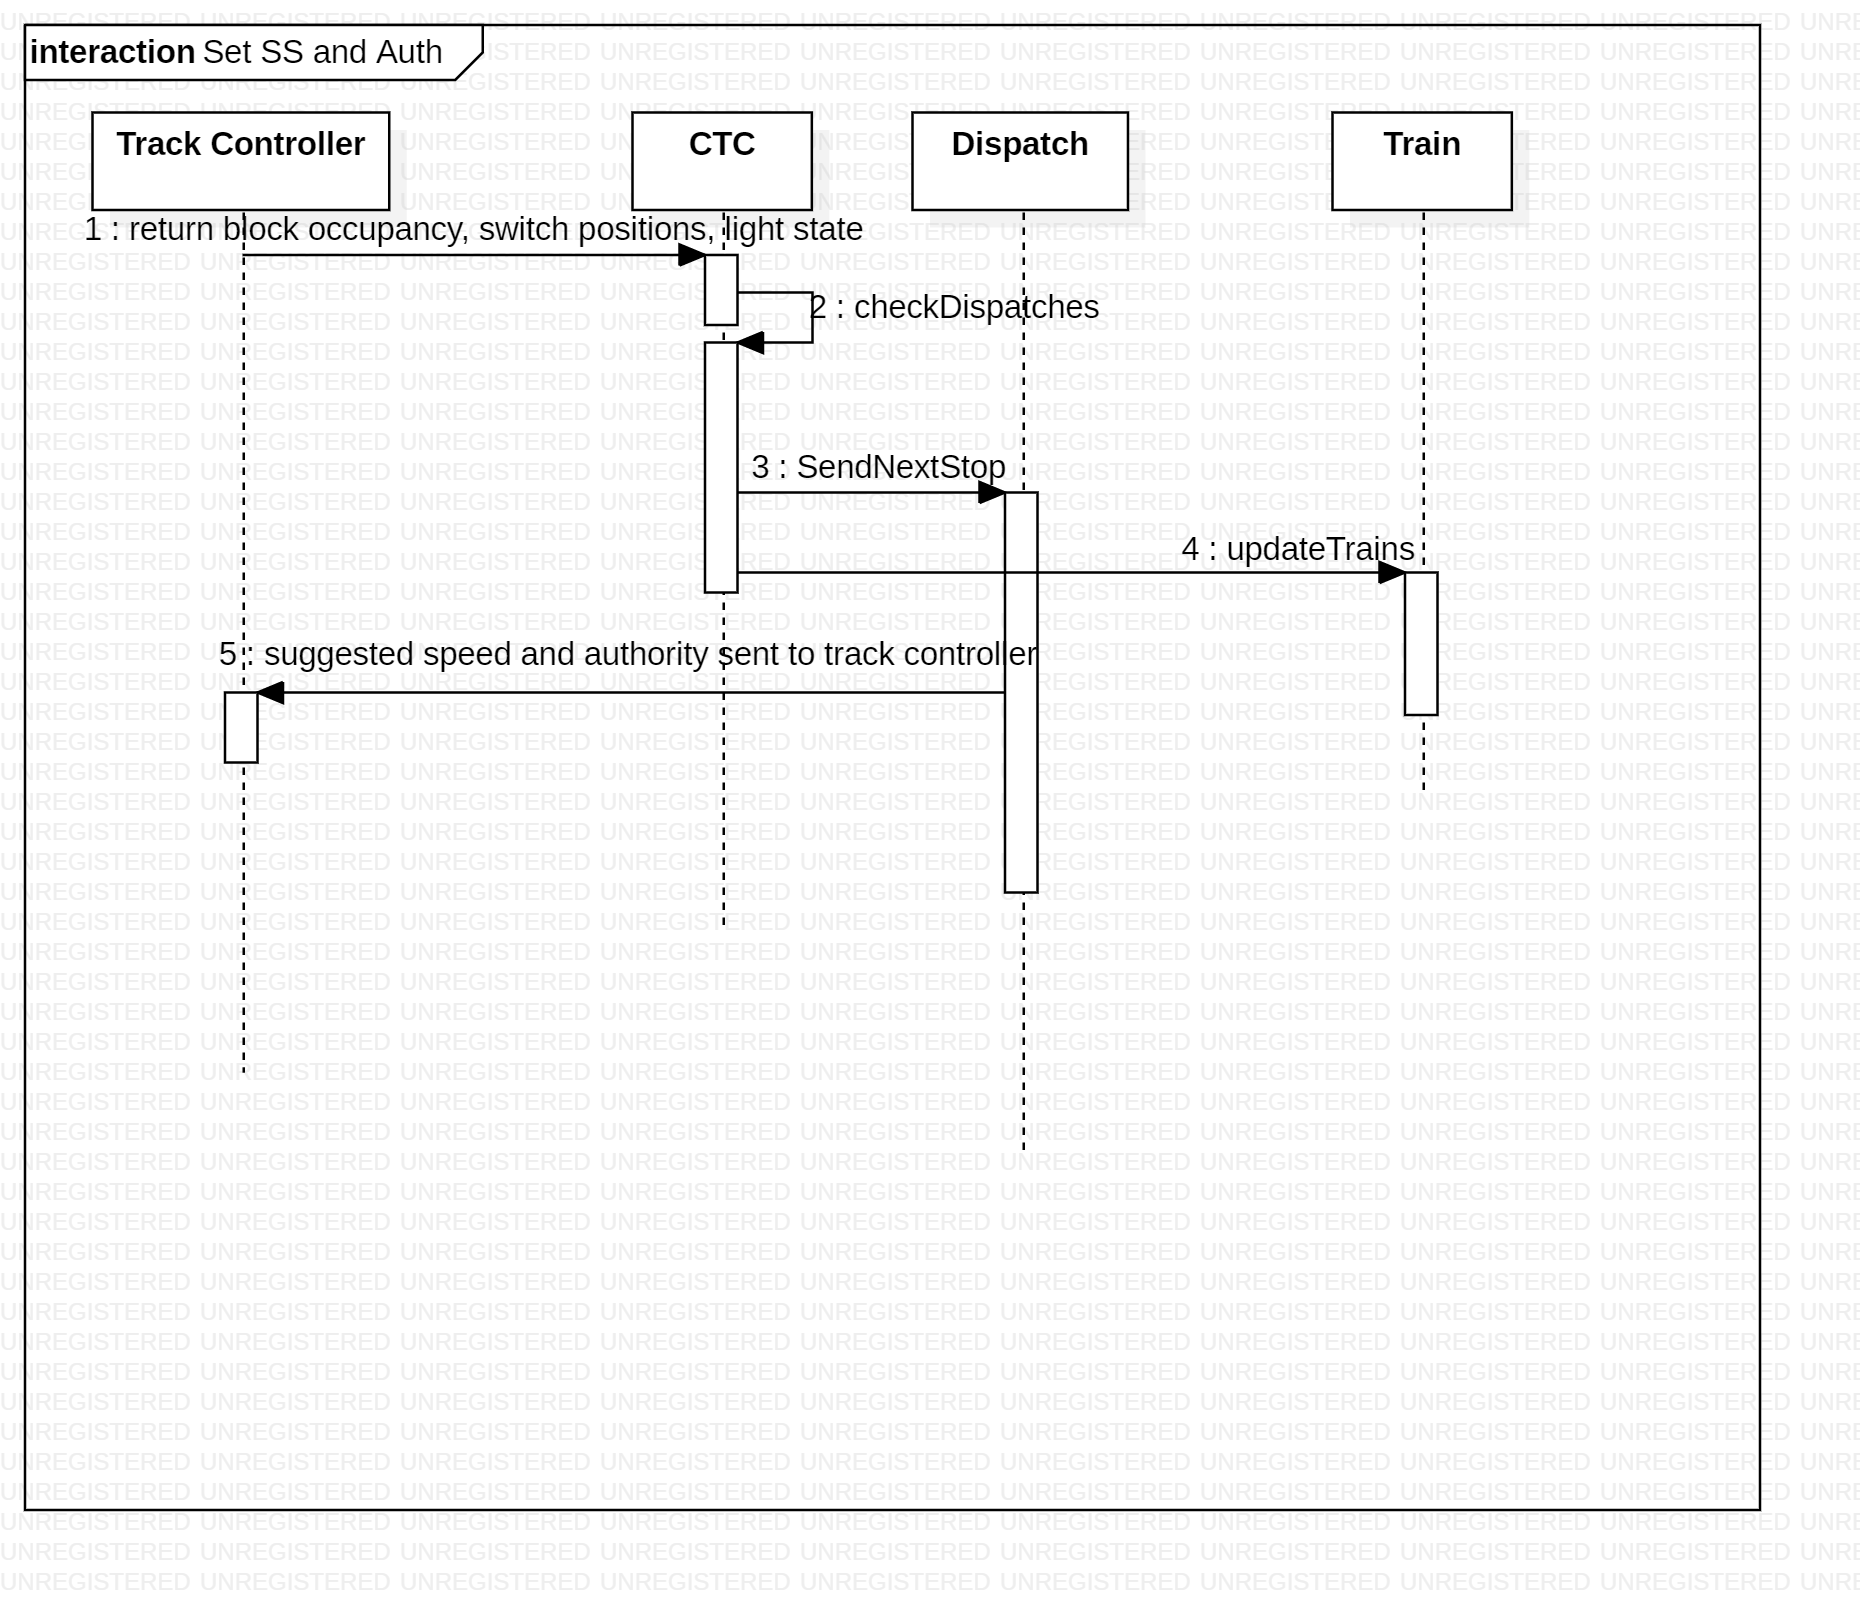
\includegraphics[width=\textwidth]{./CTC/Set_SS_and_Auth.png}
        \caption{CTC Sets a New Suggested Speed and Authority}
        \label{fig:Use Case: CTC Sets a New Suggested Speed and Authority}
    \end{figure}
     \begin{figure}[H]
        \centering
        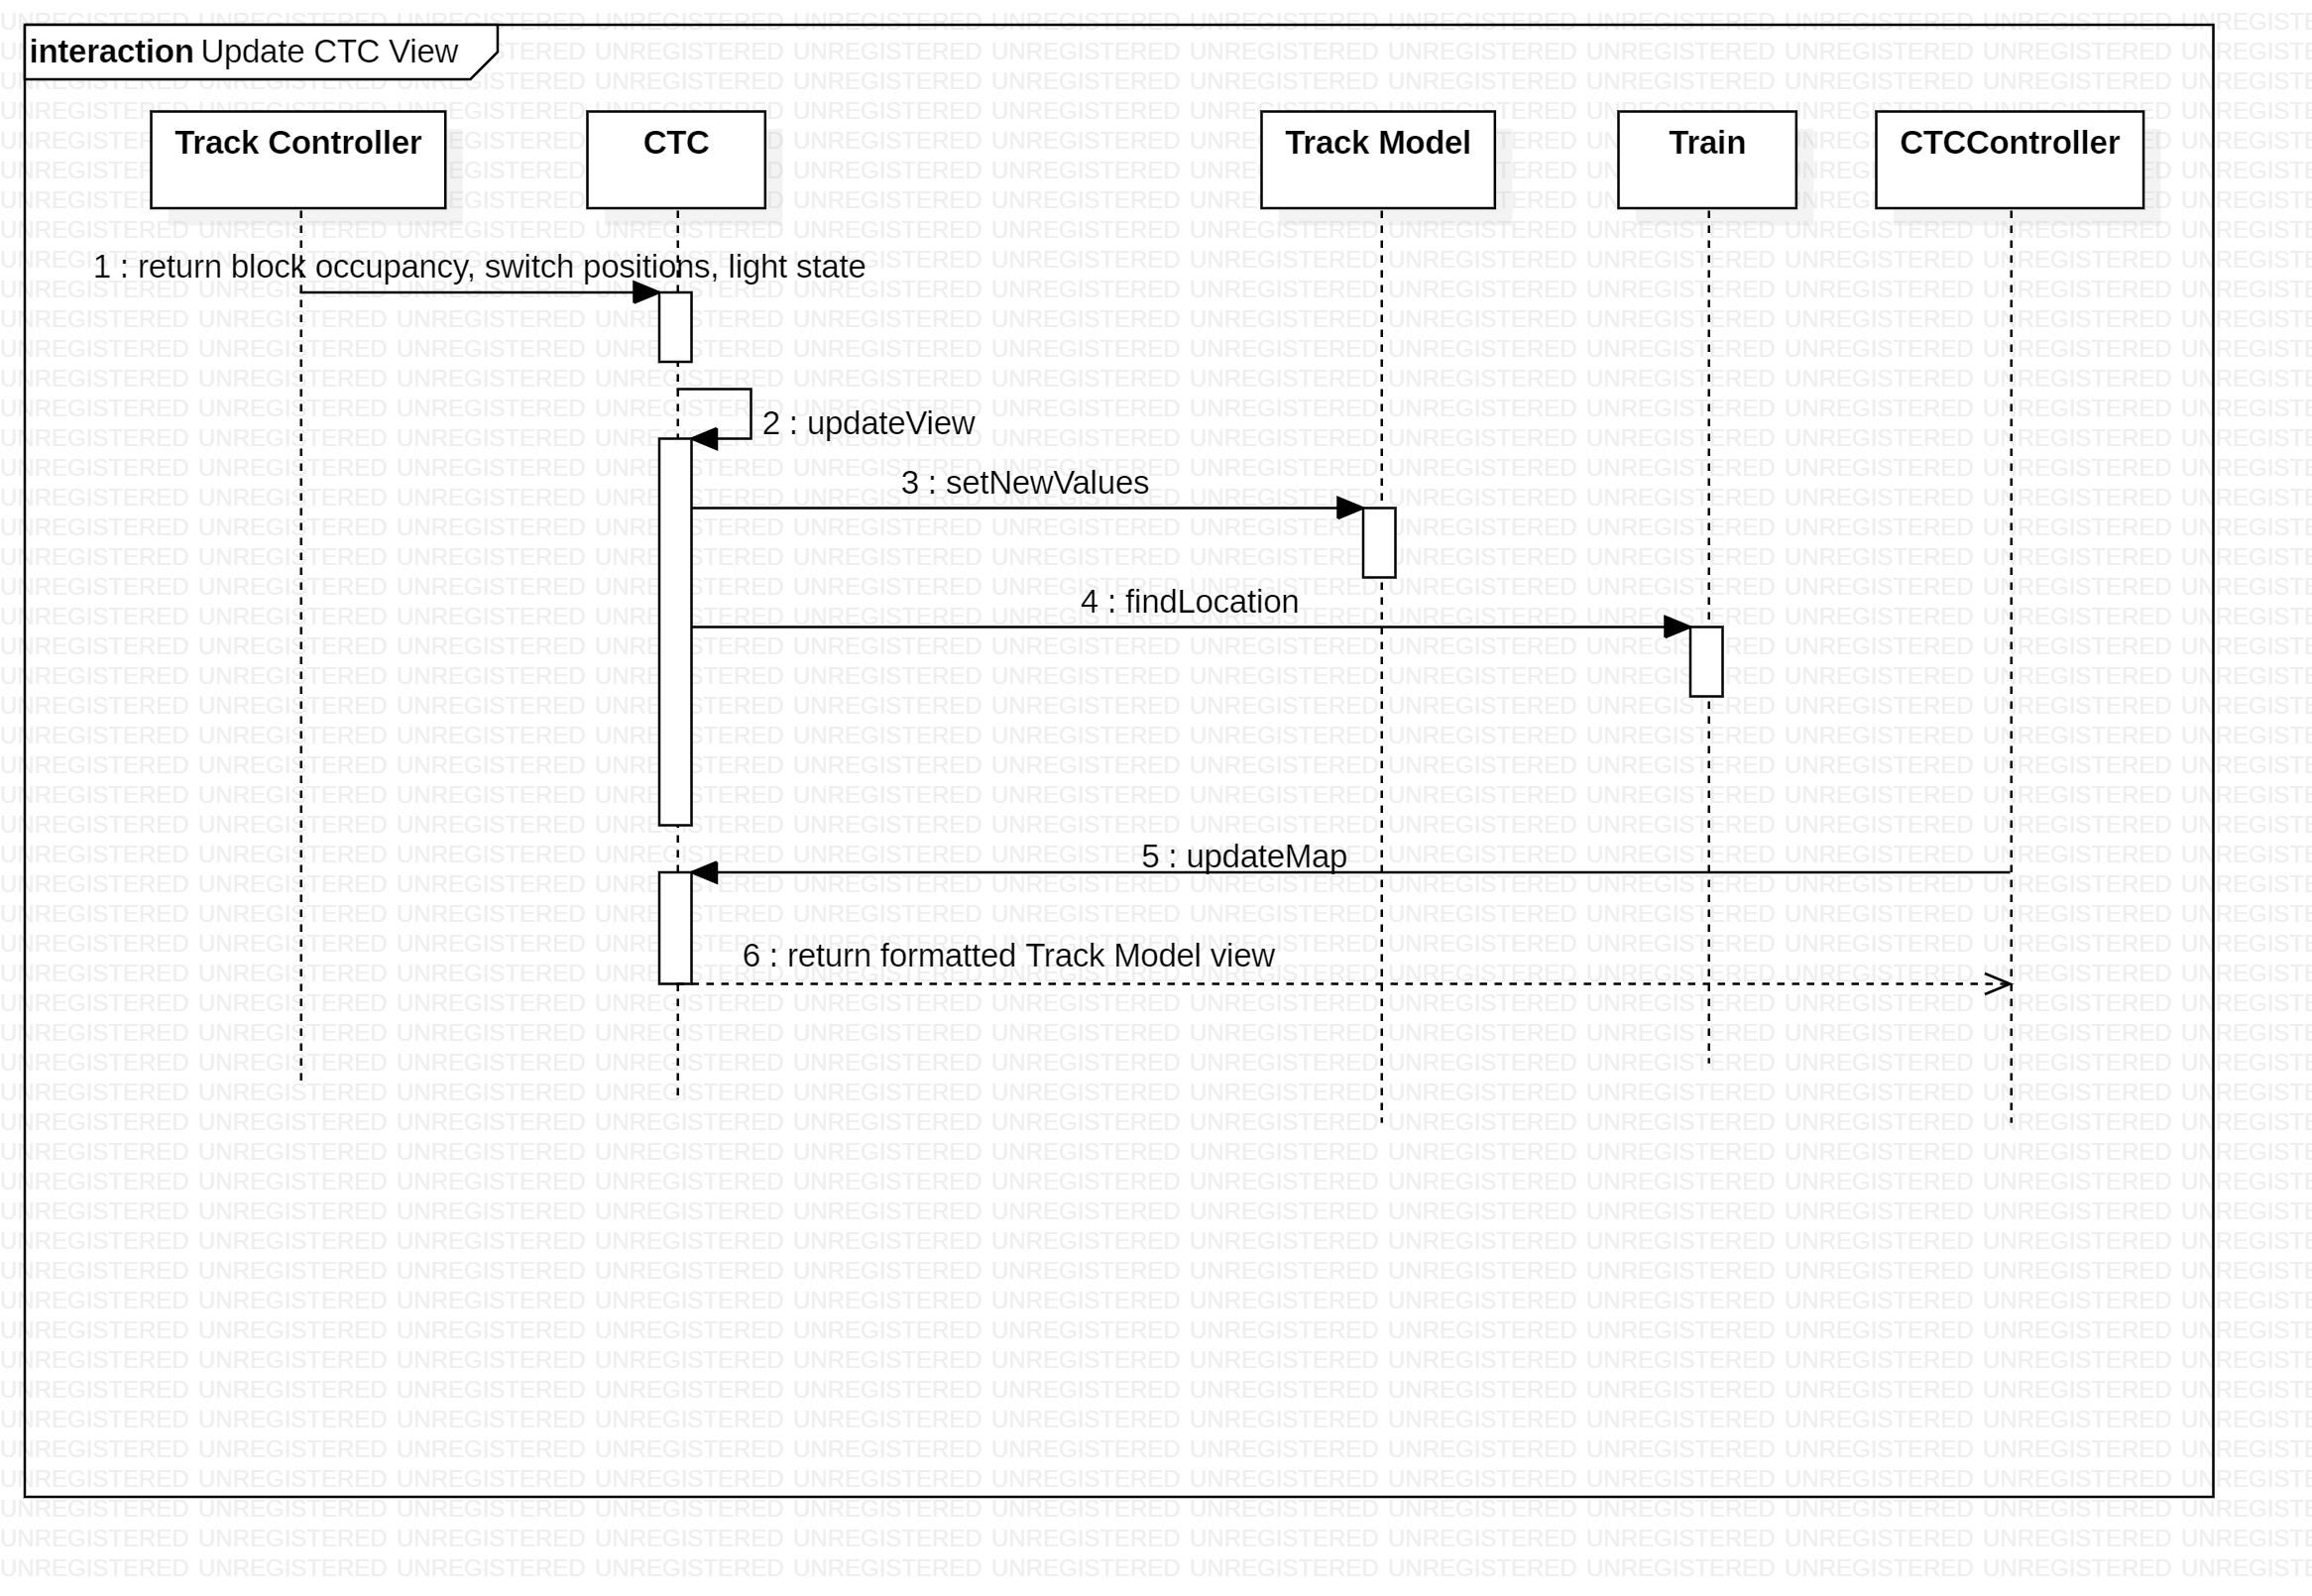
\includegraphics[width=\textwidth]{./CTC/Update_CTC_View.png}
        \caption{CTC view is updated}
        \label{fig:Use Case: CTC view is updated}
    \end{figure}
     \begin{figure}[H]
        \centering
        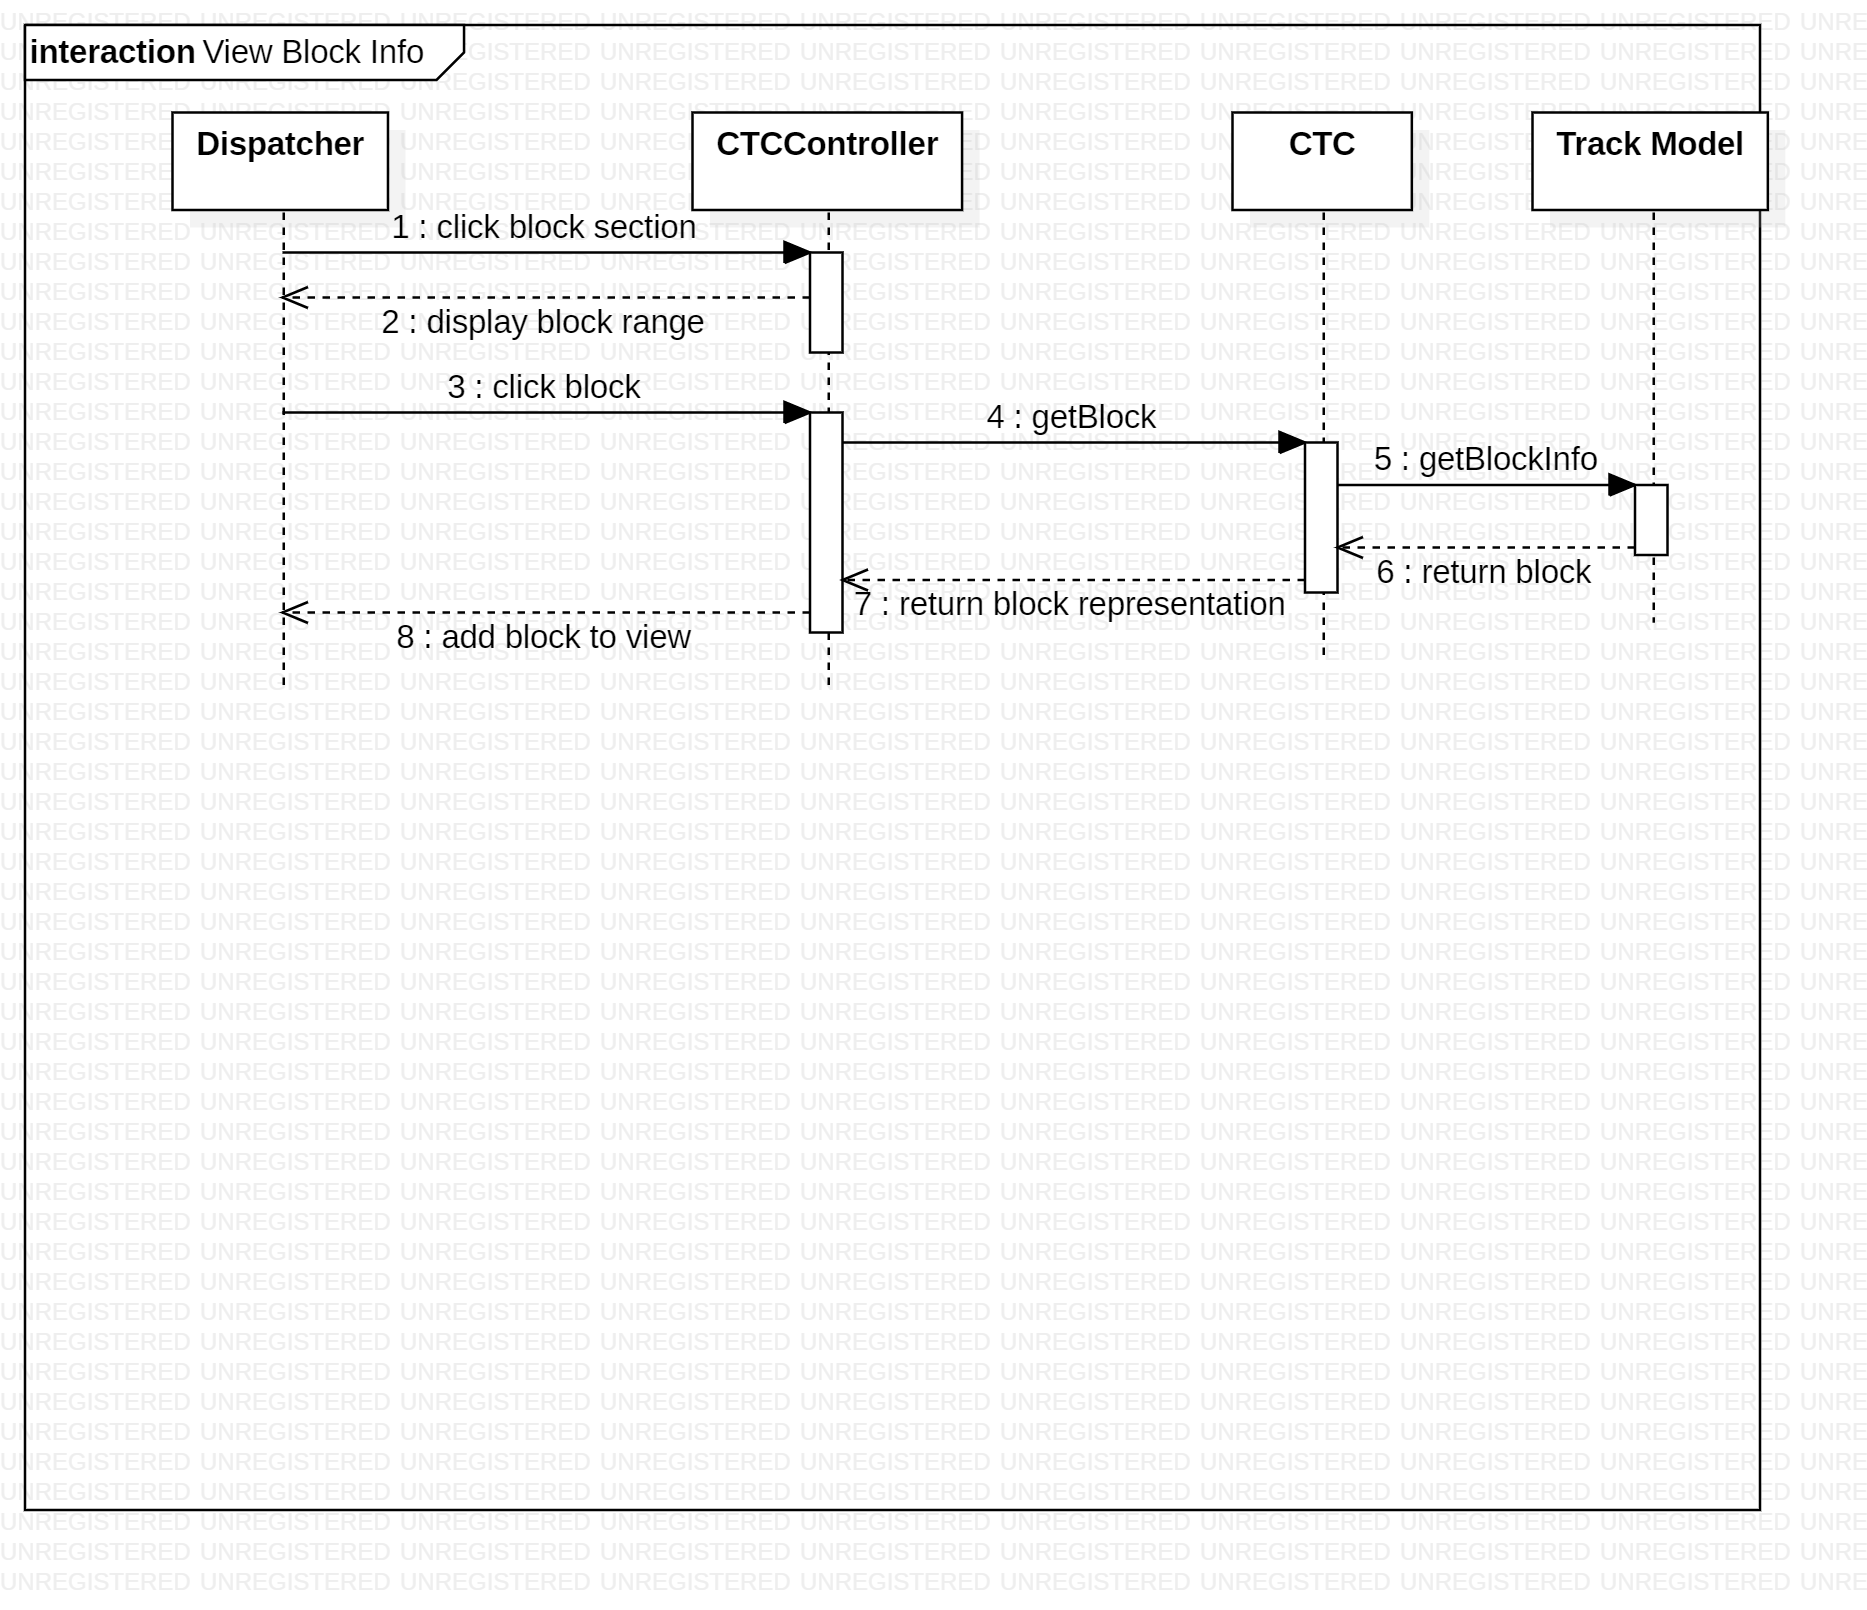
\includegraphics[width=\textwidth]{./CTC/View_Block_Info.png}
        \caption{Dispatcher Views Information for a Block}
        \label{fig:Use Case: Dispatcher Views Information for a Block}
    \end{figure}
     \begin{figure}[H]
        \centering
        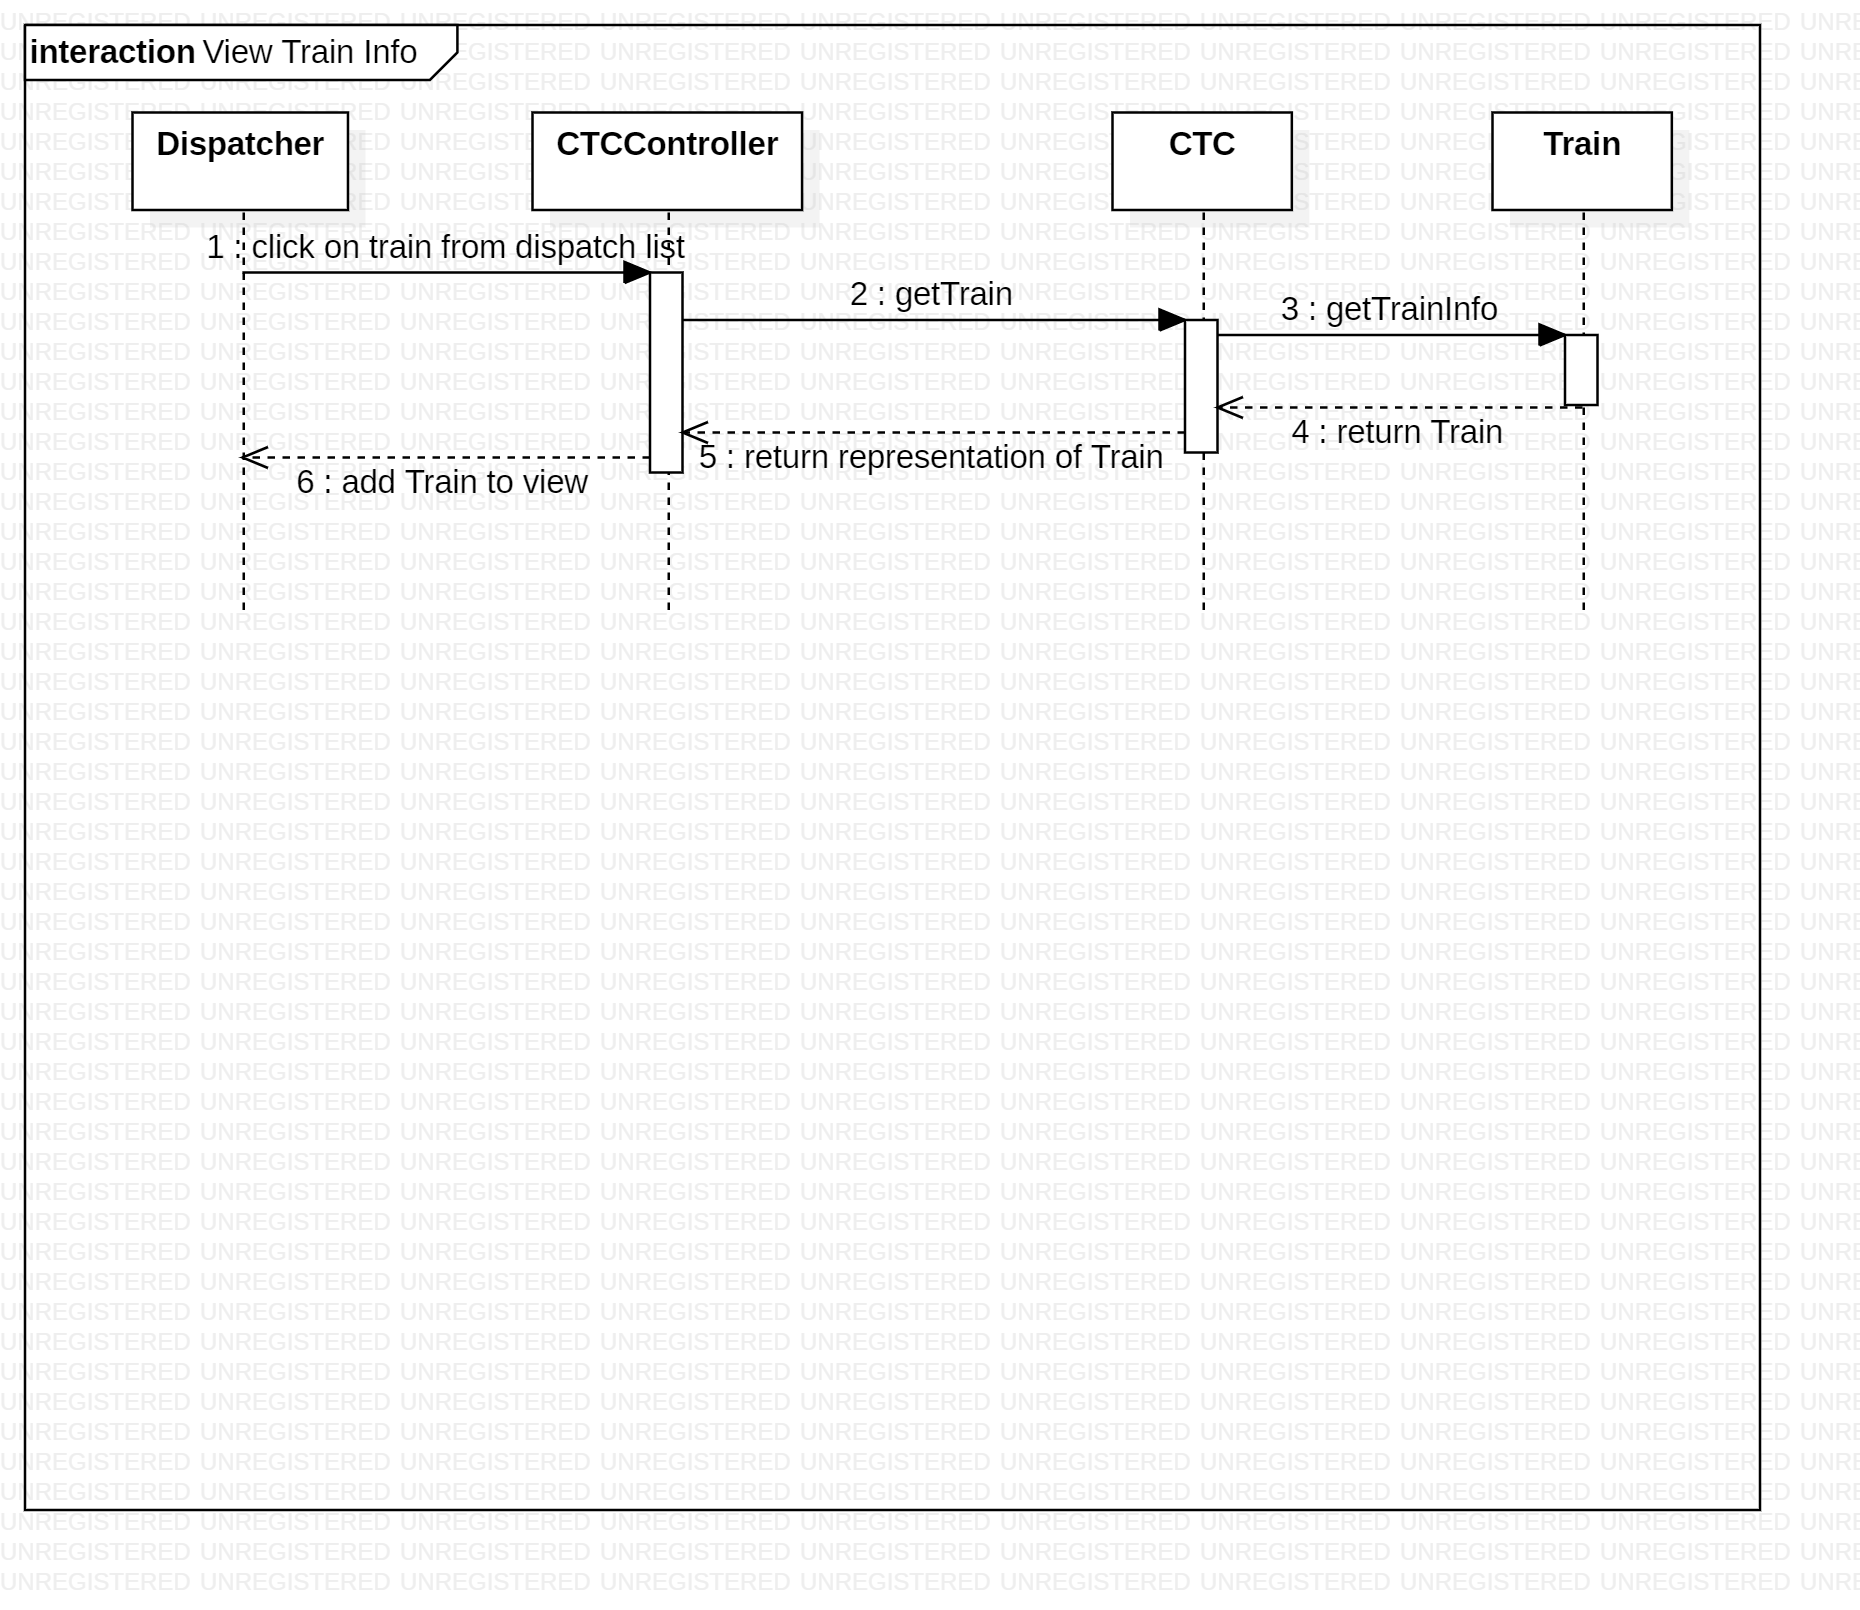
\includegraphics[width=\textwidth]{./CTC/View_Train_Info.png}
        \caption{Dispatcher Views Information for a Train}
        \label{fig:Use Case: Dispatcher Views Information for a Train}
    \end{figure}
    \paragraph{}

    \subsection{Track Controller}
    \subsubsection{Use Case Diagram}
    \begin{figure}[H]
        \centering
        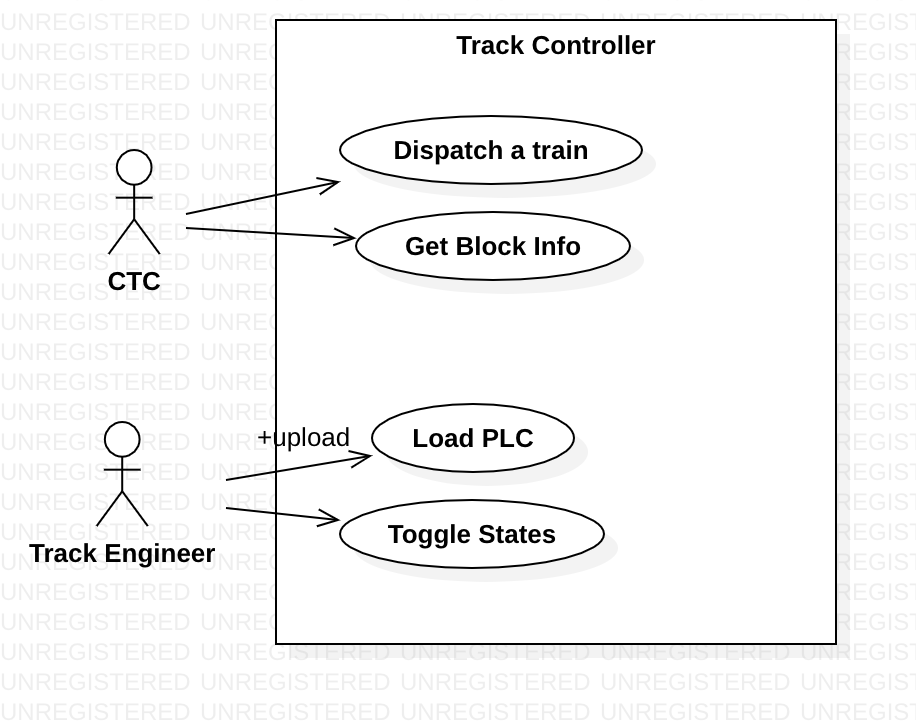
\includegraphics[width=\textwidth]{./UseCaseDiagrams/TrackController_UseCaseDiagram.png}
        \caption{Track Controller Use Cases}
        \label{fig:Track Controller Use Cases}
    \end{figure}
    \subsubsection{Use Case Descriptions}
    \paragraph{}
   \begin{longtable}{
    || >{\raggedright\arraybackslash}m{0.15 \textwidth}
    | >{\raggedright\arraybackslash}m{0.85 \textwidth}||}
    \hline
    \textbf{System} & \textbf{Track Controller} \\
    \hline
    Use Case & Upload PLC\\
    \hline
    Actors & Track Engineer\\
    \hline
    Description & \begin{itemize}
        \item Track Engineer shall upload PLC to Track Controller and set new values. 
        \item Track Controller shall pass values to the Track Model to update. 
    \end{itemize}\\
    \hline
    Data & Input: Actor Input \newline Output: Switch, lights, and railroad crossing\\
    \hline
    Stimulus & Track Engineer input\\
    \hline
    Response & Track Controller values are updated as necessary\\
    \hline
    \end{longtable}
    \begin{longtable}{
    || >{\raggedright\arraybackslash}m{0.15 \textwidth}
    | >{\raggedright\arraybackslash}m{0.85 \textwidth}||}
    \hline
    \textbf{System} & \textbf{Track Controller} \\
    \hline
    Use Case & Toggle States\\
    \hline
    Actors & Track Engineer\\
    \hline
    Description & \begin{itemize}
        \item Track Engineer toggles a switch, railroad crossing, or lights state when in maintenance mode.
        \item Track Controller shall pass values to the Track Model to update. 
    \end{itemize}\\
    \hline
    Data & Input: Actor Input \newline Output: Switch, lights, and railroad crossing\\
    \hline
    Stimulus & Track Engineer input\\
    \hline
    Response & Track Controller values are updated as necessary\\
    \hline
    \end{longtable}
    \begin{longtable}{
    || >{\raggedright\arraybackslash}m{0.15 \textwidth}
    | >{\raggedright\arraybackslash}m{0.85 \textwidth}||}
    \hline
    \textbf{System} & \textbf{Track Controller} \\
    \hline
    Use Case & Select Block\\
    \hline
    Actors & Track Engineer\\
    \hline
    Description & \begin{itemize}
        \item Track Engineer selects a Track Controller to view.
        \item Track Controller selects a block to view information
    \end{itemize}\\
    \hline
    Data & Input: Track Engineer Input \newline Output: Block Info\\
    \hline
    Stimulus & Track Engineer input\\
    \hline
    Response & Track Controller block information will be shown\\
    \hline
    \end{longtable}
    \begin{longtable}{
    || >{\raggedright\arraybackslash}m{0.15 \textwidth}
    | >{\raggedright\arraybackslash}m{0.85 \textwidth}||}
    \hline
    \textbf{System} & \textbf{Track Controller} \\
    \hline
    Use Case & Get suggested speed and authority\\
    \hline
    Actors & Track Controller, CTC \\
    \hline
    Description & \begin{itemize}
        \item CTC sends an authority and suggested speed to the Track Controller
        \item Track Controller shall pass this information to the track model to update
    \end{itemize}\\
    \hline
    Data & Input: CTC Input \newline Output: Suggested Speed, Authority\\
    \hline
    Stimulus & CTC input\\
    \hline
    Response & New suggested speed and authority shall be updated\\
    \hline
    \end{longtable}
    \begin{longtable}{
    || >{\raggedright\arraybackslash}m{0.15 \textwidth}
    | >{\raggedright\arraybackslash}m{0.85 \textwidth}||}
    \hline
    \textbf{System} & \textbf{Track Controller} \\
    \hline
    Use Case & Update Maintenance Mode\\
    \hline
    Actors & Track Controller, CTC \\
    \hline
    Description & \begin{itemize}
        \item CTC sends an authority of -1 to a block in the Track Controller
        \item Track Controller shall pass this information to the track model to update
        \item Track Controller shall close the block as necessary
    \end{itemize}\\
    \hline
    Data & Input: Authority \newline Output: Boolean for success or failure to close block\\
    \hline
    Stimulus & CTC input\\
    \hline
    Response & Block is either closed or open\\
    \hline
    \end{longtable}
    \subsubsection{Class Diagrams}
    \begin{figure}[H]
        \centering
        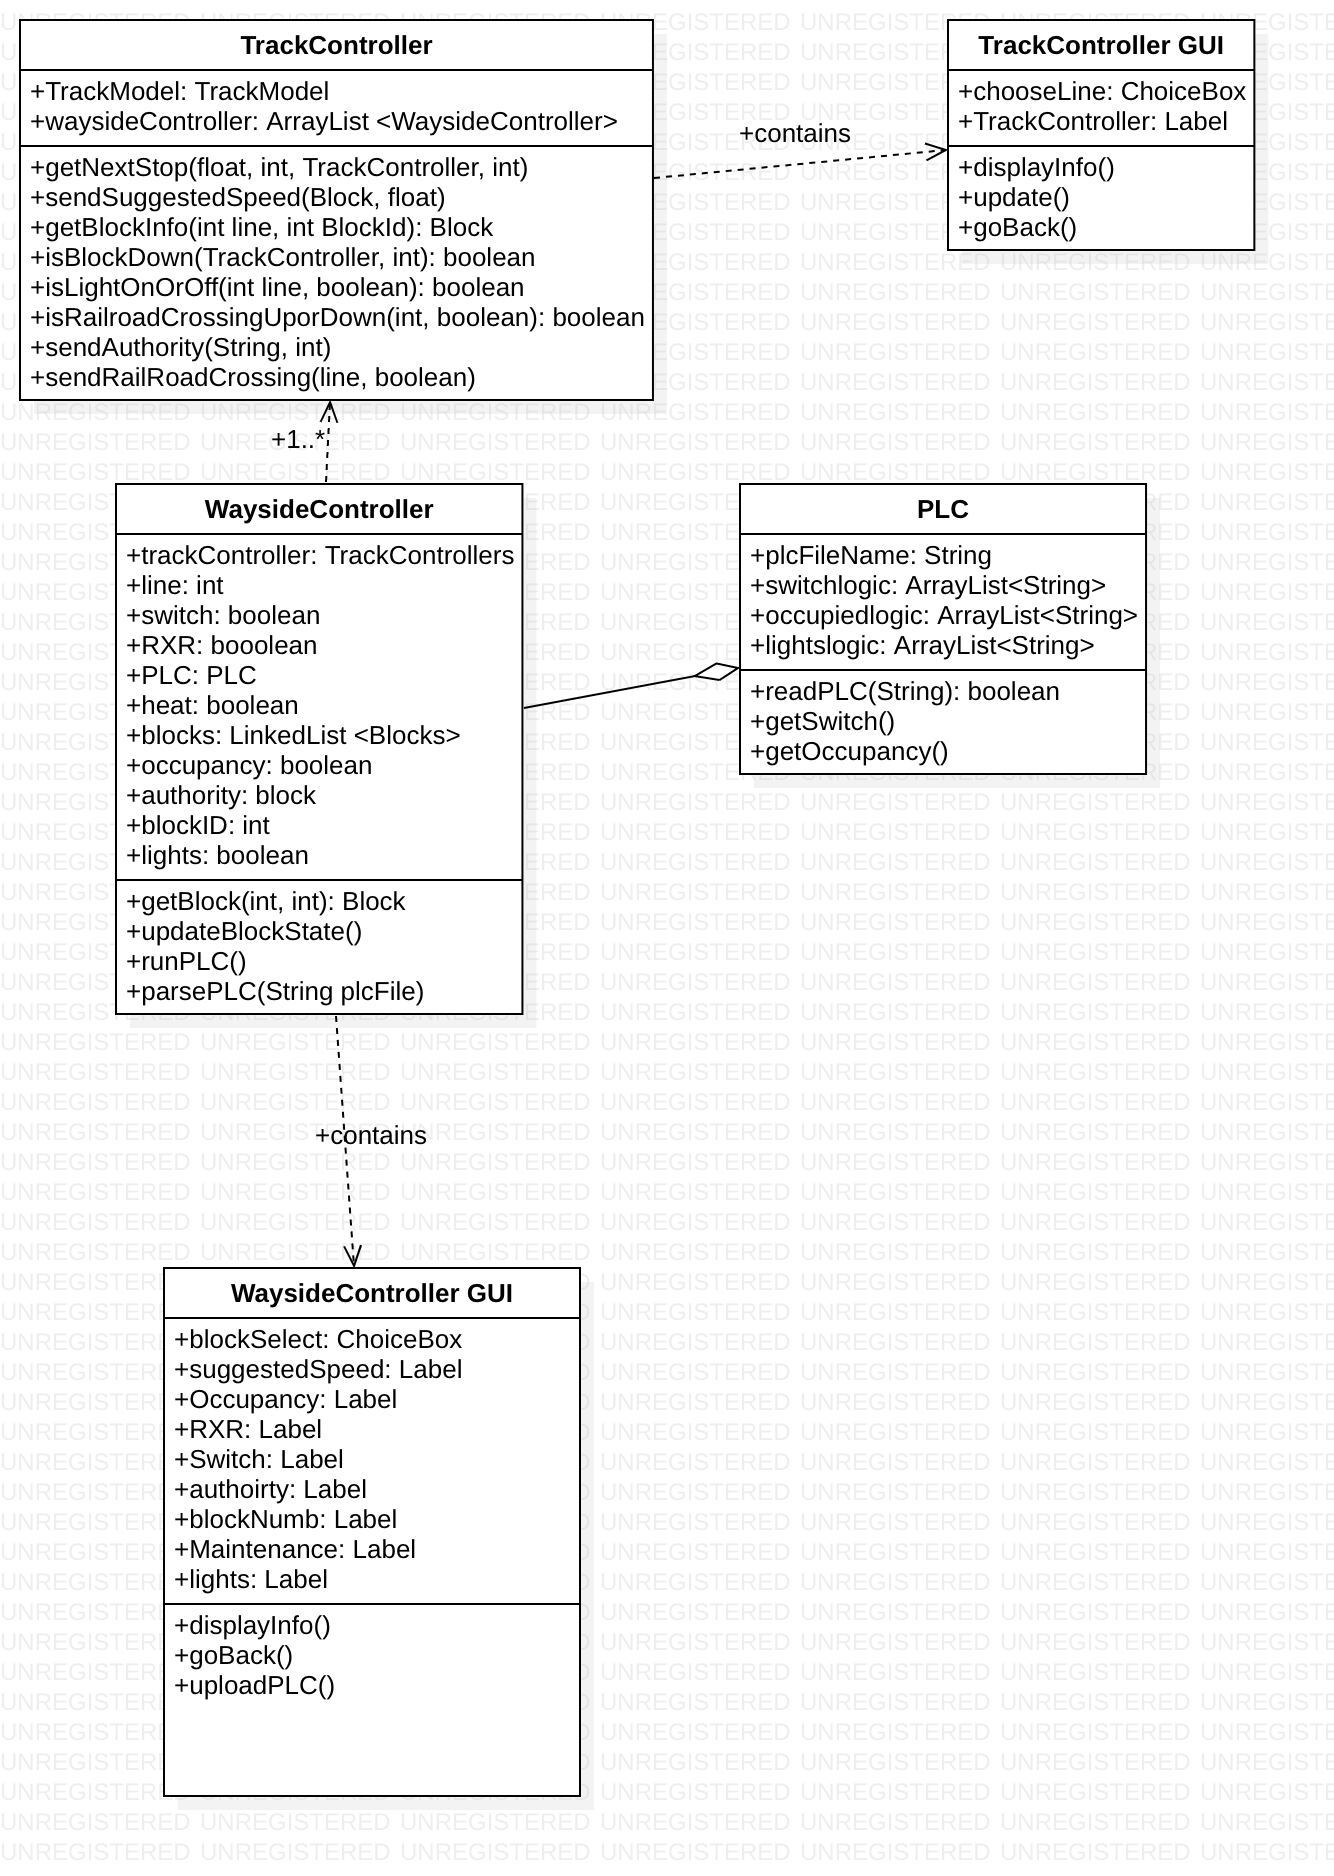
\includegraphics[width=\textwidth]{./ClassDiagrams/TrackController_ClassDiagram.png}
        \caption{Use Case: Track Controller Class Diagram}
        \label{fig:Track Controller Class Diagram}
    \end{figure}
    \subsubsection{Sequence Diagrams}
    \begin{figure}[H]
        \centering
        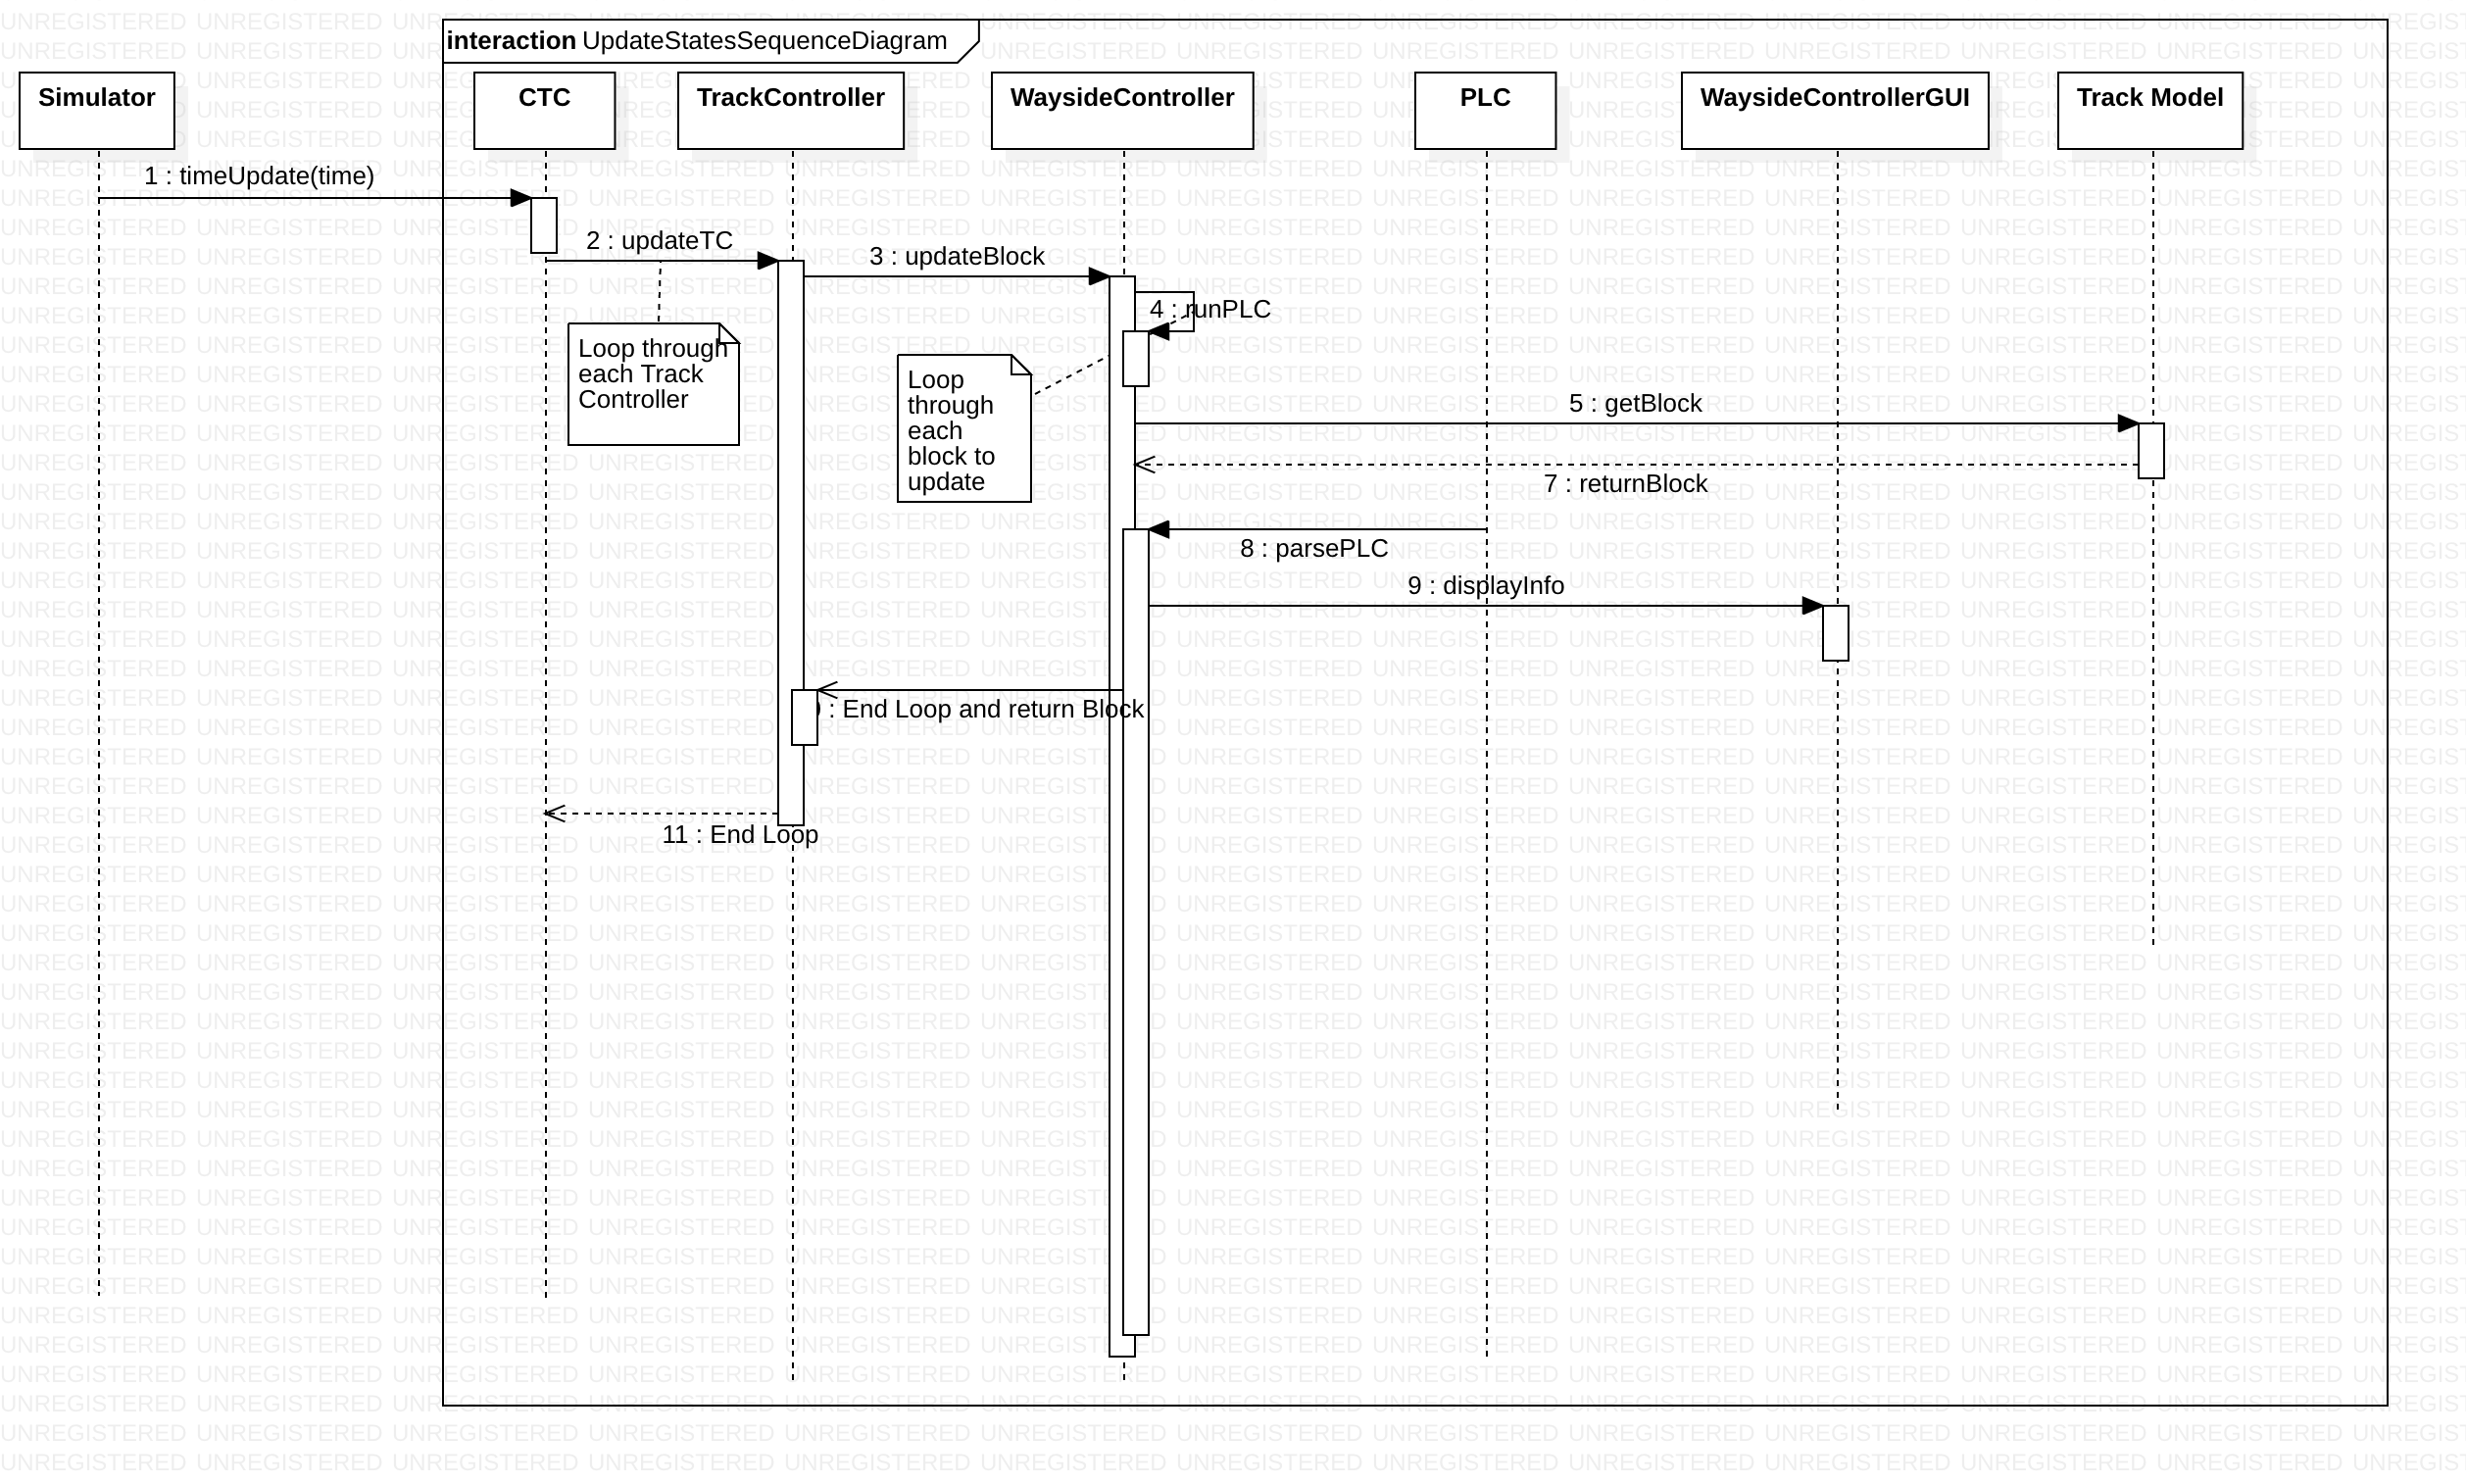
\includegraphics[width=\textwidth]{./SequenceDiagrams/UpdateStatesSequenceDiagram.png}
        \caption{Use Case: Track Controller Update States}
        \label{fig: Use Case: Track Controller Update States}
    \end{figure}
    \begin{figure}[H]
        \centering
        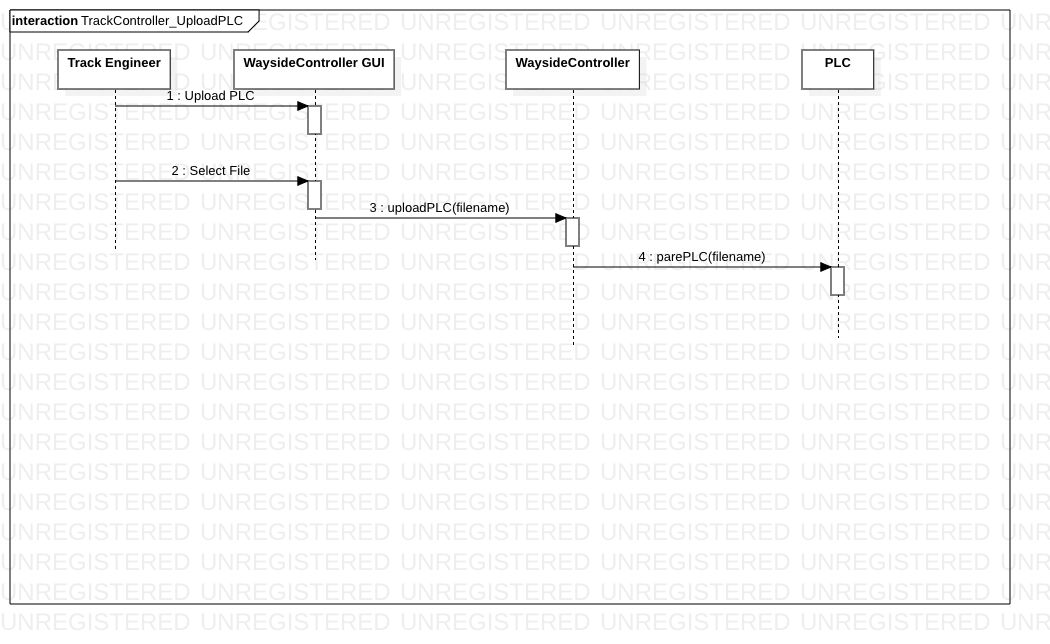
\includegraphics[width=\textwidth]{./SequenceDiagrams/TrackController_UploadPLC.png}
        \caption{Use Case: Track Controller Update PLC}
        \label{fig: Use Case: Track Controller Update PLC}
    \end{figure}
    \begin{figure}[H]
        \centering
        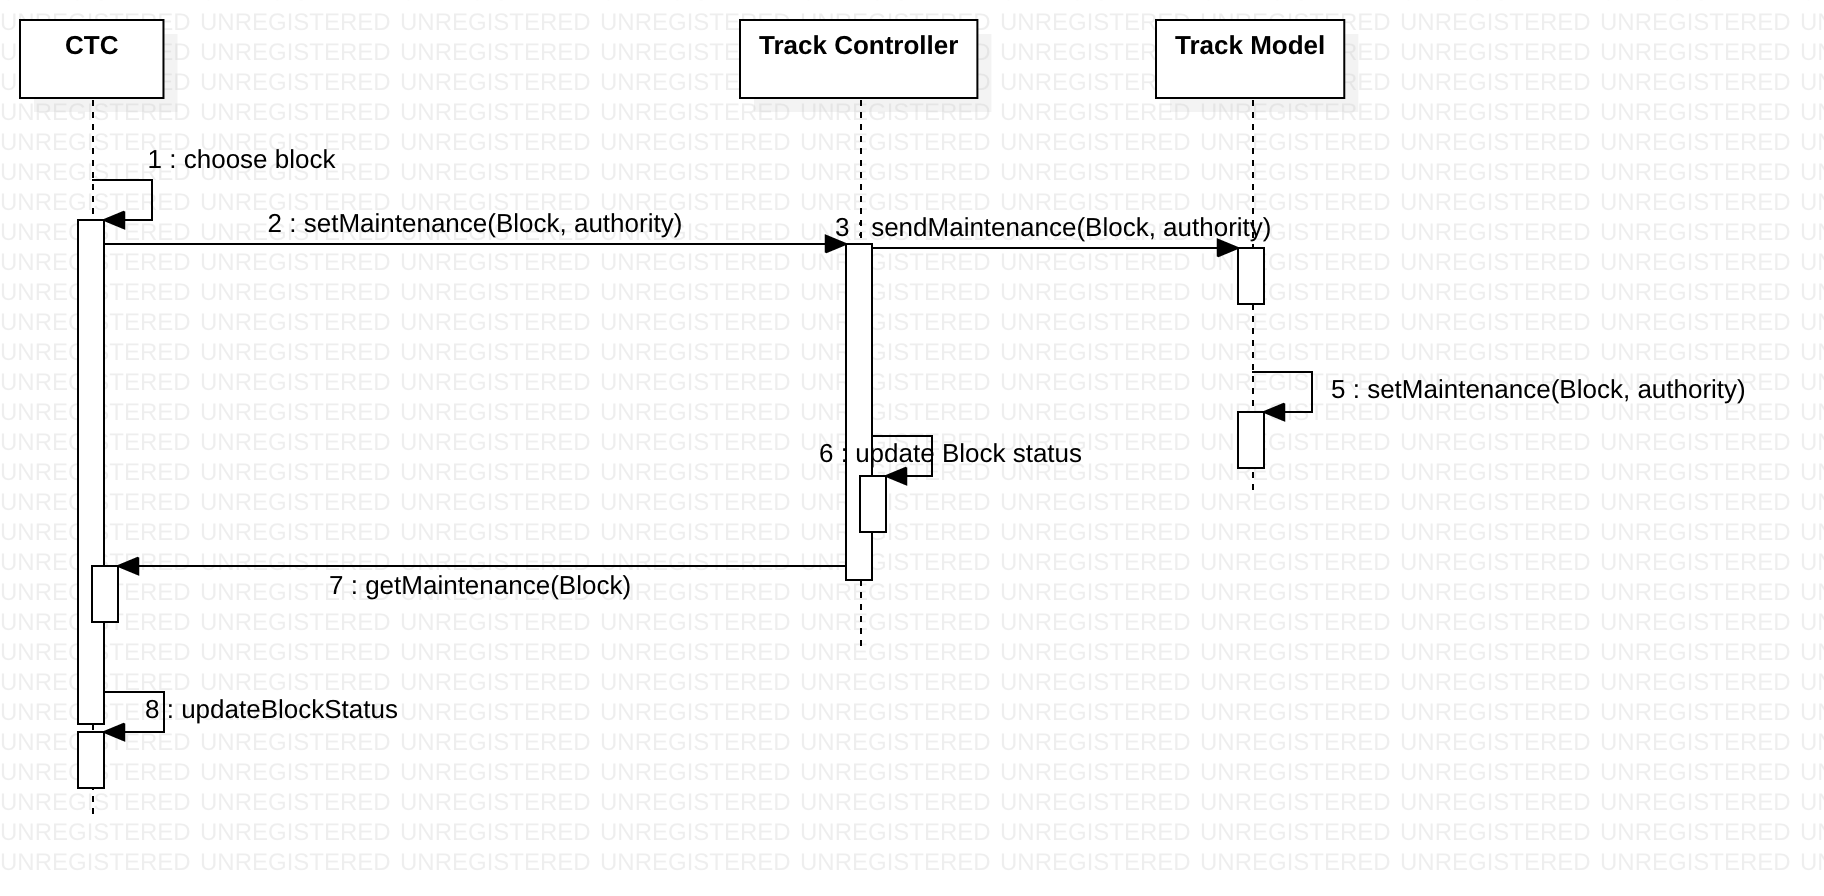
\includegraphics[width=\textwidth]{./SequenceDiagrams/TrackController_UpdateMaintenance.png}
        \caption{Use Case: Track Controller Update Maintenance}
        \label{fig: Use Case: Track Controller Update Maintenance Mode}
    \end{figure}
    \begin{figure}[H]
        \centering
        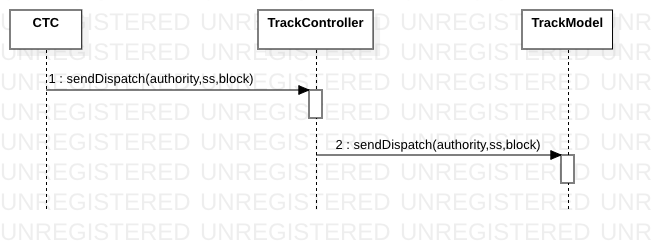
\includegraphics[width=\textwidth]{./SequenceDiagrams/TrackController_Dispatch.png}
        \caption{Use Case: Track Controller Set Authority and Suggested Speed}
        \label{fig:Track Controller Get Suggested Speed and Authority}
    \end{figure}
    \begin{figure}[H]
        \centering
        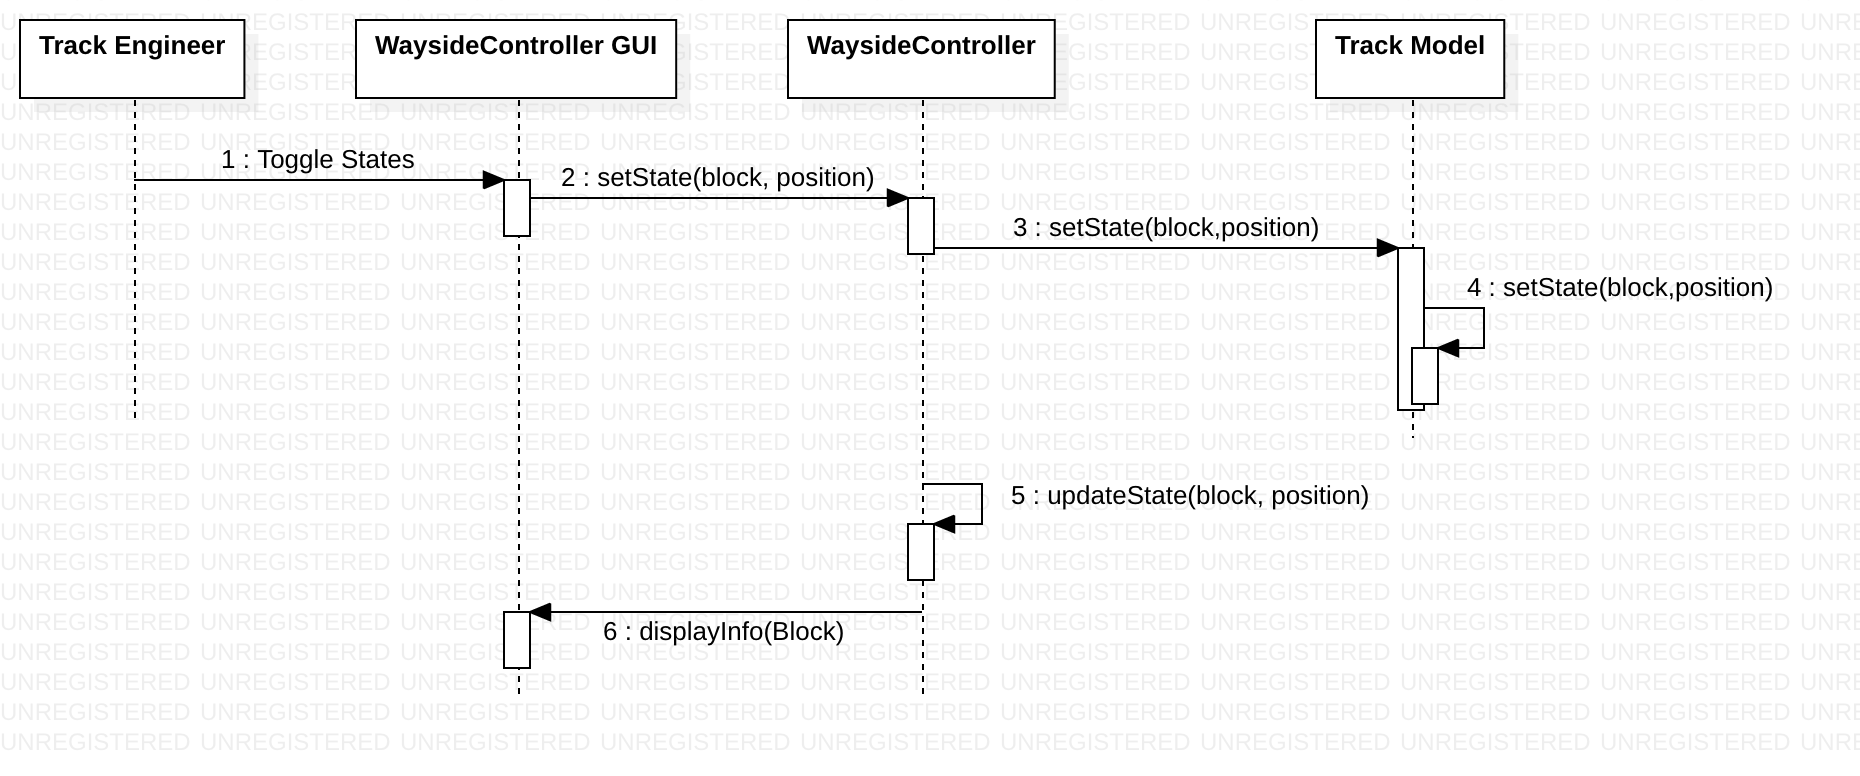
\includegraphics[width=\textwidth]{./SequenceDiagrams/TrackController_ToggleState.png}
        \caption{Use Case: Track Controller Toggle State}
        \label{fig: Use Case: Track Controller Toggle States}
    \end{figure}
    \begin{figure}[H]
        \centering
        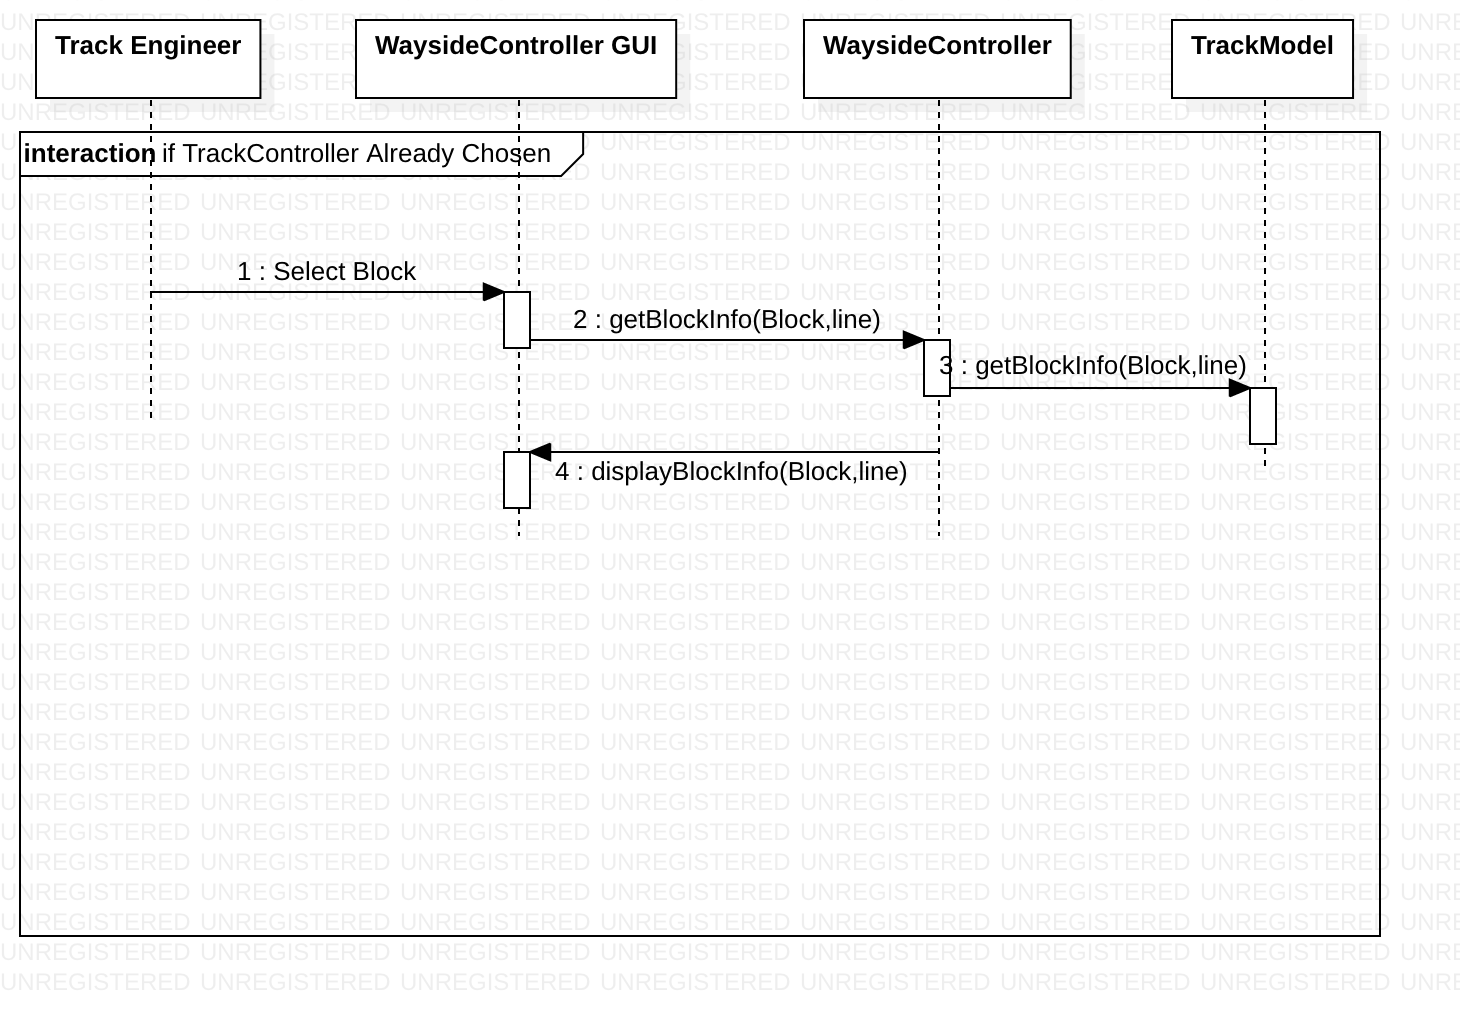
\includegraphics[width=\textwidth]{./SequenceDiagrams/TrackController_SelectBlock.png}
        \caption{Track Controller Select Block}
        \label{fig: Use Case: Track Controller Select Block}
    \end{figure}

    \subsection{Track Model}
    
    \subsubsection{Use Case Diagram}
    \begin{figure}[H]
        \centering
        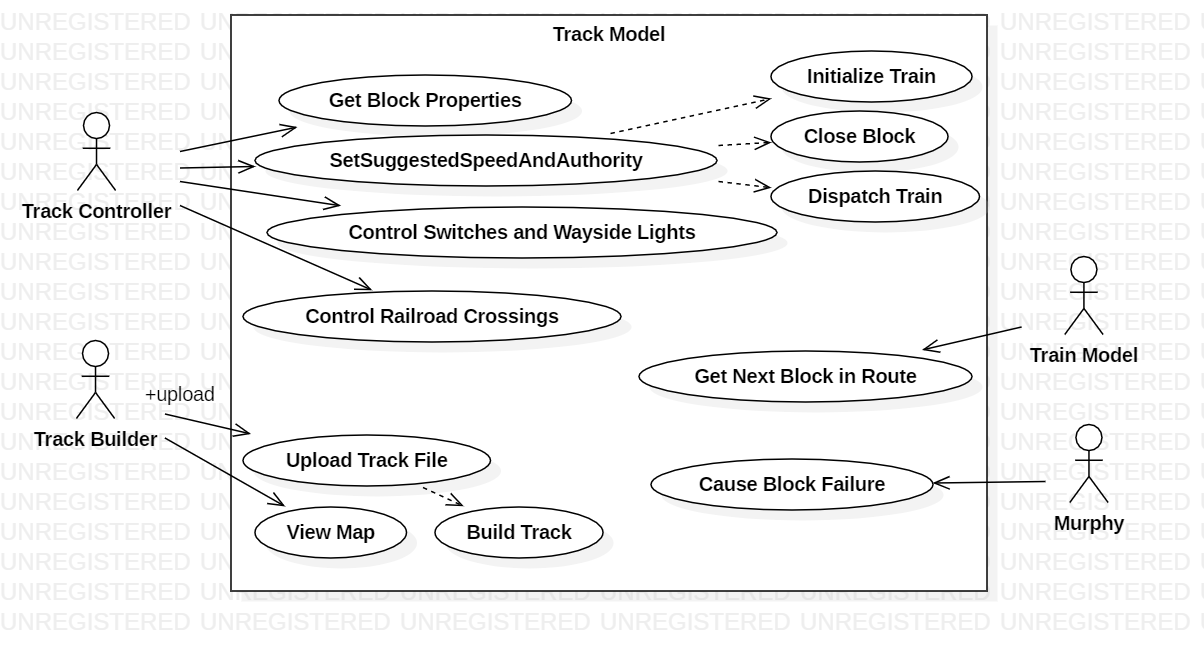
\includegraphics[width=\textwidth]{./UseCaseDiagrams/TrackModel_UseCaseDiagram_Pic.png}
        \caption{Track Model Use Cases}
        \label{fig:Track Model Use Cases}
    \end{figure}
    
    
    \subsubsection{Use Case Descriptions}
    \begin{longtable}{
    || >{\raggedright\arraybackslash}m{0.15 \textwidth}
    | >{\raggedright\arraybackslash}m{0.85 \textwidth}||}
    \hline
    \textbf{System} & \textbf{Track Model} \\
    \hline
    Use Case & Build track from track file\\
    \hline
    Actors & Track Builder\\
    \hline
    Description & \begin{itemize}
        \item Track Builder uploads track file
        \item Track Model builds track by parsing file
        \item Track Model performs verification on the built track
        \item Track Builder confirms built track looks correct
    \end{itemize}\\
    \hline
    Data & Input: Formatted track file \newline Output: Track object\\
    \hline
    Stimulus & Module initialization\\
    \hline
    Response & Track object is constructed and ready to be used\\
    \hline
    \end{longtable}
    
    \begin{longtable}{
    || >{\raggedright\arraybackslash}m{0.15 \textwidth}
    | >{\raggedright\arraybackslash}m{0.85 \textwidth}||}
    \hline
    \textbf{System} & \textbf{Track Model} \\
    \hline
    Use Case & Track Controller closes block for maintenance
    \hline
    Actors & Track Controller\\
    \hline
    Description & \begin{itemize}
        \item Track Controller gives command to close block
        \item Track Model searches for reference to desired block
        \item Track Controller sends block non-functional suggested speed and authority (e.g -1) as an encoding to close block
        \item Block state is set to closed
    \end{itemize}\\
    \hline
    Data & Input: Suggested speed, authority, boolean value signifying opening/closing block\newline Output: Boolean for success or failure to close block\\
    \hline
    Stimulus & Method call from Track Controller\\
    \hline
    Response & Block is either opened or closed for maintenance\\
    \hline
    \end{longtable}
    
    \begin{longtable}{
    || >{\raggedright\arraybackslash}m{0.15 \textwidth}
    | >{\raggedright\arraybackslash}m{0.85 \textwidth}||}
    \hline
    \textbf{System} & \textbf{Track Model} \\
    \hline
    Use Case & Cause block failure\\
    \hline
    Actors & Train Controller\\
    \hline
    Description & \begin{itemize}
        \item Murphy issues command to cause block failure
        \item Track Model searches for reference to desired block
        \item setFailure(int) called on block to create failure
    \end{itemize}\\
    \hline
    Data & Input: Block number, failure type \newline Output: Boolean signifying success\\
    \hline
    Stimulus & Method call from Murphy\\
    \hline
    Response & Block status is updated to show failure\\
    \hline
    \end{longtable}
    
    \begin{longtable}{
    || >{\raggedright\arraybackslash}m{0.15 \textwidth}
    | >{\raggedright\arraybackslash}m{0.85 \textwidth}||}
    \hline
    \textbf{System} & \textbf{Track Model} \\
    \hline
    Use Case & Control RXR\\
    \hline
    Actors & Train Controller\\
    \hline
    Description & \begin{itemize}
        \item Track Controller issues command to change state of railroad crossing
        \item Track Model searches for reference to desired block
        \item setDown(boolean) called on RXR of block to change state
    \end{itemize}\\
    \hline
    Data & Input: Block number, commanded RXR state \newline Output: n/a\\
    \hline
    Stimulus & Method call from Track Controller\\
    \hline
    Response & RXR status is updated\\
    \hline
    \end{longtable}
    
    \begin{longtable}{
    || >{\raggedright\arraybackslash}m{0.15 \textwidth}
    | >{\raggedright\arraybackslash}m{0.85 \textwidth}||}
    \hline
    \textbf{System} & \textbf{Track Model} \\
    \hline
    Use Case & Control Switches and Wayside Lights\\
    \hline
    Actors & Train Controller\\
    \hline
    Description & \begin{itemize}
        \item Track Controller issues command to change state of switch and corresponding wayside lights
        \item Track Model searches for reference to desired block
        \item setOrientation(boolean) and setLights(boolean) called on switch and lights of block to change state
    \end{itemize}\\
    \hline
    Data & Input: Block number, commanded switch orientation, command light state state \newline Output: n/a\\
    \hline
    Stimulus & Method call from Track Controller\\
    \hline
    Response & Switch and light statuses are updated\\
    \hline
    \end{longtable}
    
    \begin{longtable}{
    || >{\raggedright\arraybackslash}m{0.15 \textwidth}
    | >{\raggedright\arraybackslash}m{0.85 \textwidth}||}
    \hline
    \textbf{System} & \textbf{Track Model} \\
    \hline
    Use Case & Train Model Requests Next Block in Path\\
    \hline
    Actors & Train Model\\
    \hline
    Description & \begin{itemize}
        \item Train Model requests reference to next block on it's route
        \item Track model returns the reference to the next block
    \end{itemize}\\
    \hline
    Data & Input: Train's current block \newline Output: Train's next block on path\\
    \hline
    Stimulus & Train detects polarity switch in track circuit (leaves current block)\\
    \hline
    Response & Train now has reference to new current block and can use its properties in it's force calculations\\
    \hline
    \end{longtable}
    
    \begin{longtable}{
    || >{\raggedright\arraybackslash}m{0.15 \textwidth}
    | >{\raggedright\arraybackslash}m{0.85 \textwidth}||}
    \hline
    \textbf{System} & \textbf{Track Model} \\
    \hline
    Use Case & Track Controller Initializes Train\\
    \hline
    Actors & Train Controller\\
    \hline
   Description & \begin{itemize}
        \item Track Controller gives command to initialize new train
        \item Track Model searches for reference to desired block (should always be the start block for this command)
        \item Track Controller sends block non-functional suggested speed and authority (e.g -1) as an encoding to initialize a new train
    \end{itemize}\\
    \hline
    Data & Input: Suggested speed, authority to encode command to initialize train \newline Output: Boolean signifying success\\
    \hline
    Stimulus & Method call from Track Controller\\
    \hline
    Response & Train Model instance is created and ready to be dispatched\\
    \hline
    \end{longtable}
    
    \begin{longtable}{
    || >{\raggedright\arraybackslash}m{0.15 \textwidth}
    | >{\raggedright\arraybackslash}m{0.85 \textwidth}||}
    \hline
    \textbf{System} & \textbf{Track Model} \\
    \hline
    Use Case & Track Controller Dispatches Train\\
    \hline
    Actors & Train Controller\\
    \hline
   Description & \begin{itemize}
        \item Track Controller gives command to dispatch train
        \item Track Model searches for reference to desired block
        \item Track Controller sends block a functional (non-negative) suggested speed and authority to be passed into the train occupying the block
    \end{itemize}\\
    \hline
    Data & Input: Block number, suggested speed, authority \newline Output: Boolean signifying success\\
    \hline
    Stimulus & Method call from Track Controller\\
    \hline
    Response & Train Model occupying block updated with new suggested speed and authority\\
    \hline
    \end{longtable}
    
    \subsubsection{Class Diagram}
    \begin{figure}[H]
        \centering
        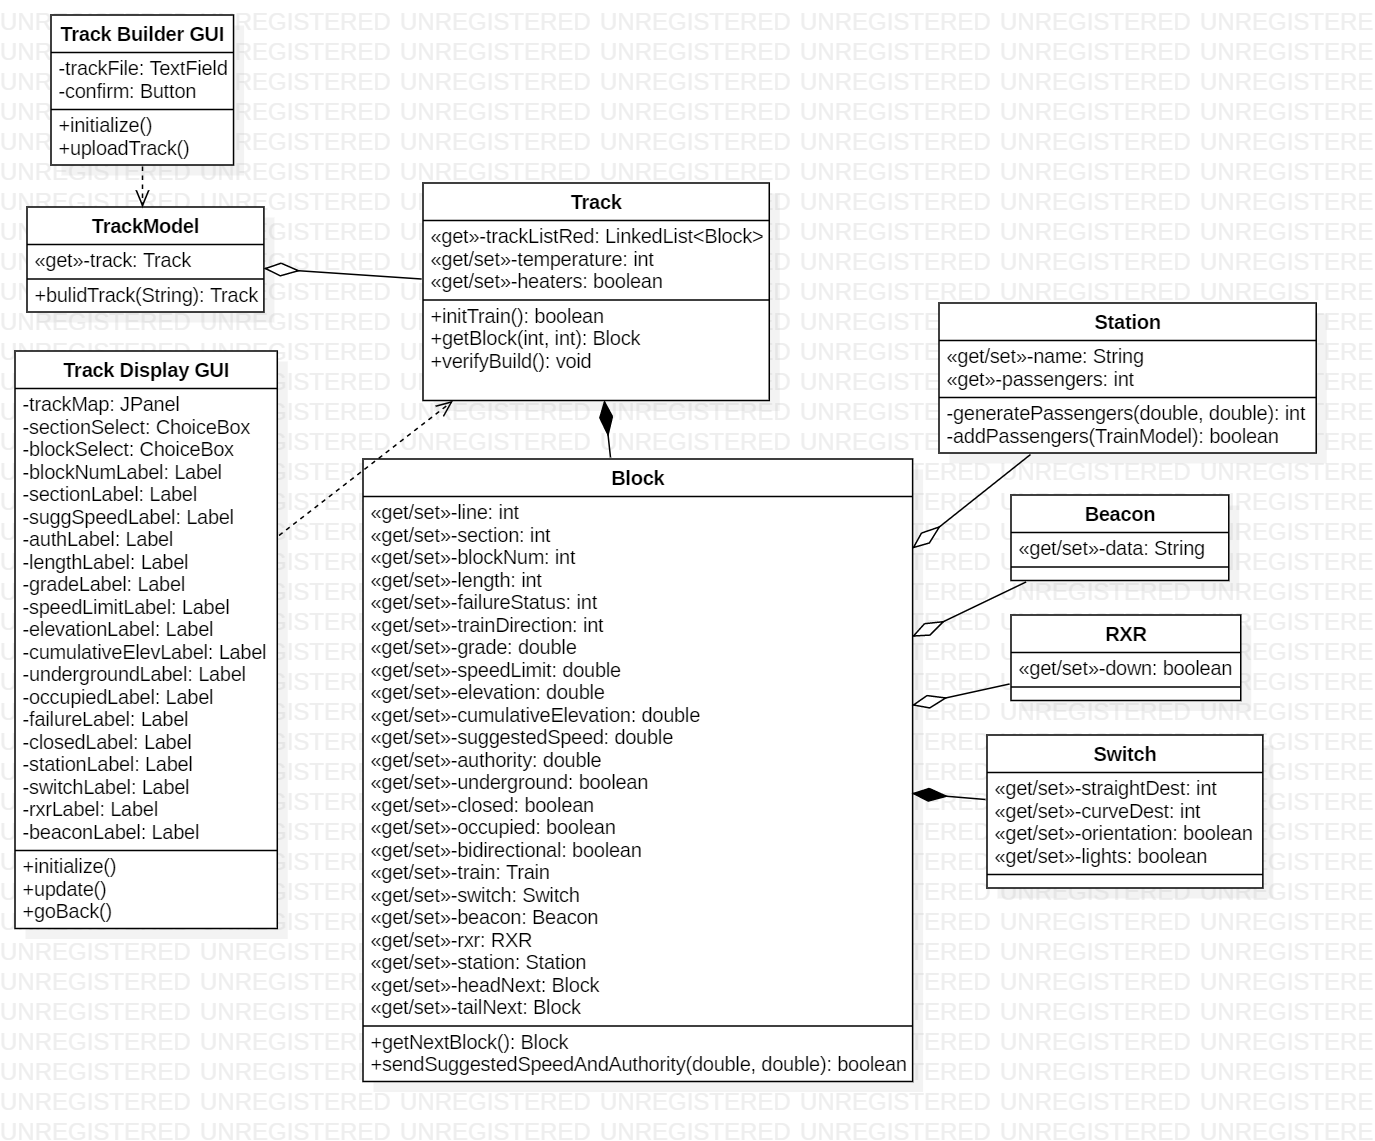
\includegraphics[width=\textwidth]{./ClassDiagrams/TrackModel_ClassDiagram_pic.png}
        \caption{Track Model Class Diagram}
        \label{fig:Track Model Class Diagram}
    \end{figure}
    
    \subsubsection{Sequence Diagrams}
    \begin{figure}[H]
        \centering
        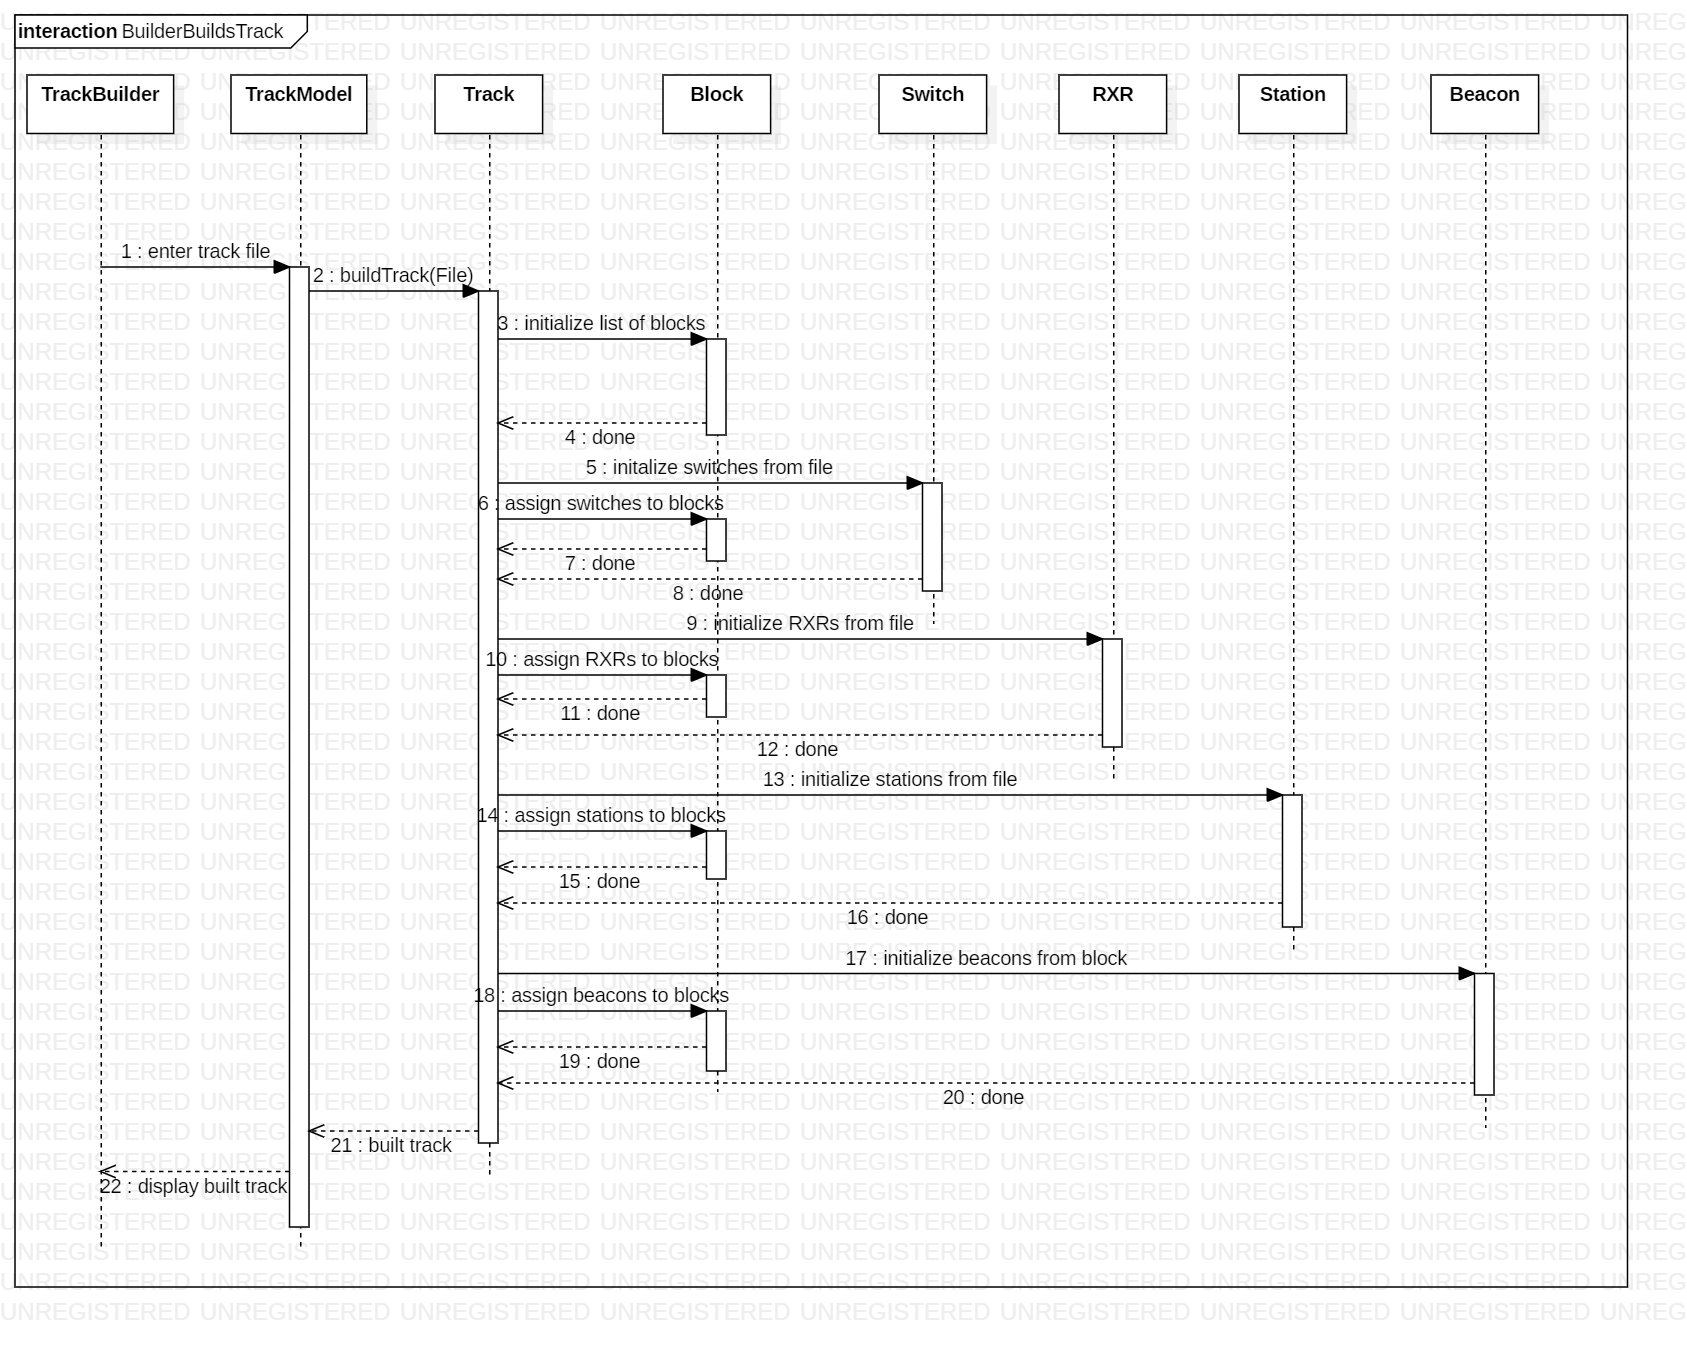
\includegraphics[width=\textwidth]{./SequenceDiagrams/TrackModel_SeqDiagrams/TrackModel_SeqDiagram_BuilderBuildsTrack.png}
        \caption{Use Case: Track Builder builds track using track layout file}
        \label{fig:Track Builder Builds Track}
    \end{figure}
    \begin{figure}[H]
        \centering
        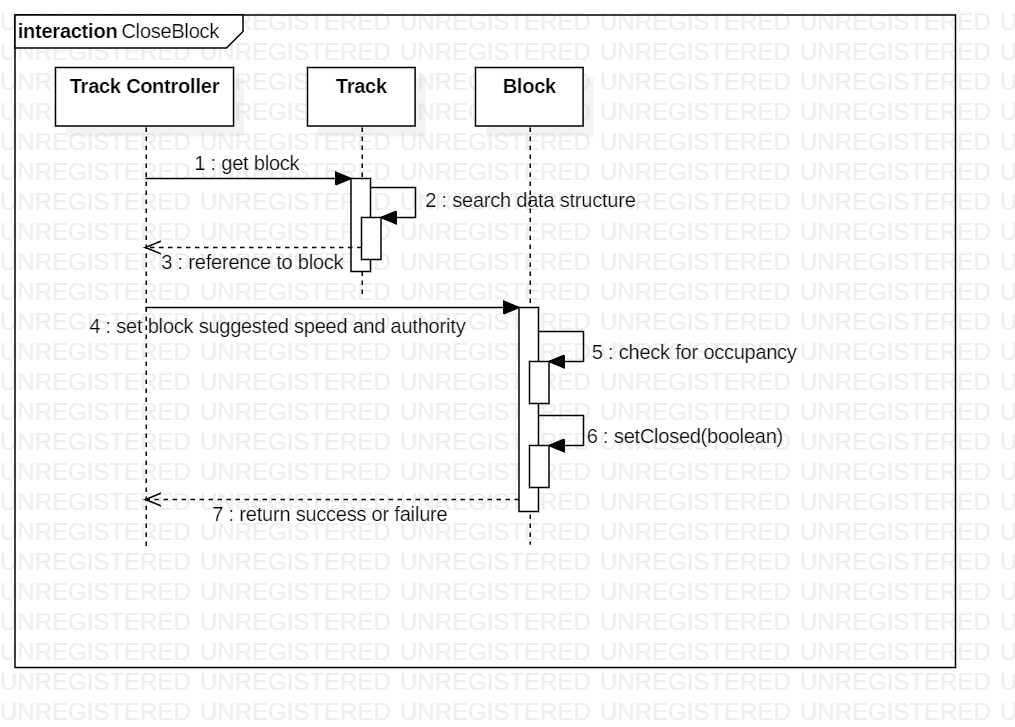
\includegraphics[width=\textwidth]{./SequenceDiagrams/TrackModel_SeqDiagrams/TrackModel_SeqDiagram_CloseBlock.png}
        \caption{Use Case: Track Controller closes block for maintenance}
        \label{fig:Track Controller Closes Block}
    \end{figure}
    \begin{figure}[H]
        \centering
        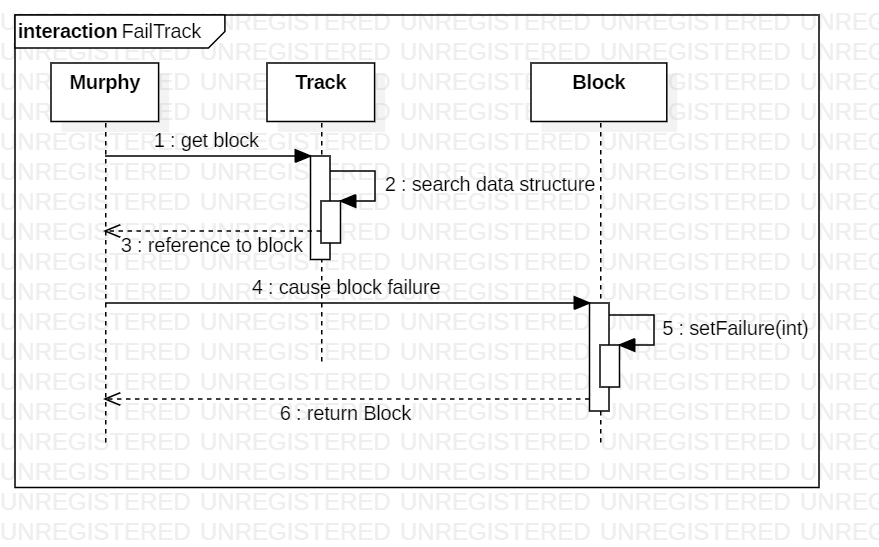
\includegraphics[width=\textwidth]{./SequenceDiagrams/TrackModel_SeqDiagrams/TrackModel_SeqDiagram_MurphyFailsBlock.png}
        \caption{Use Case: Murphy Causes Block to Fail}
        \label{fig:Murphy Fails Block}
    \end{figure}
    \begin{figure}[H]
        \centering
        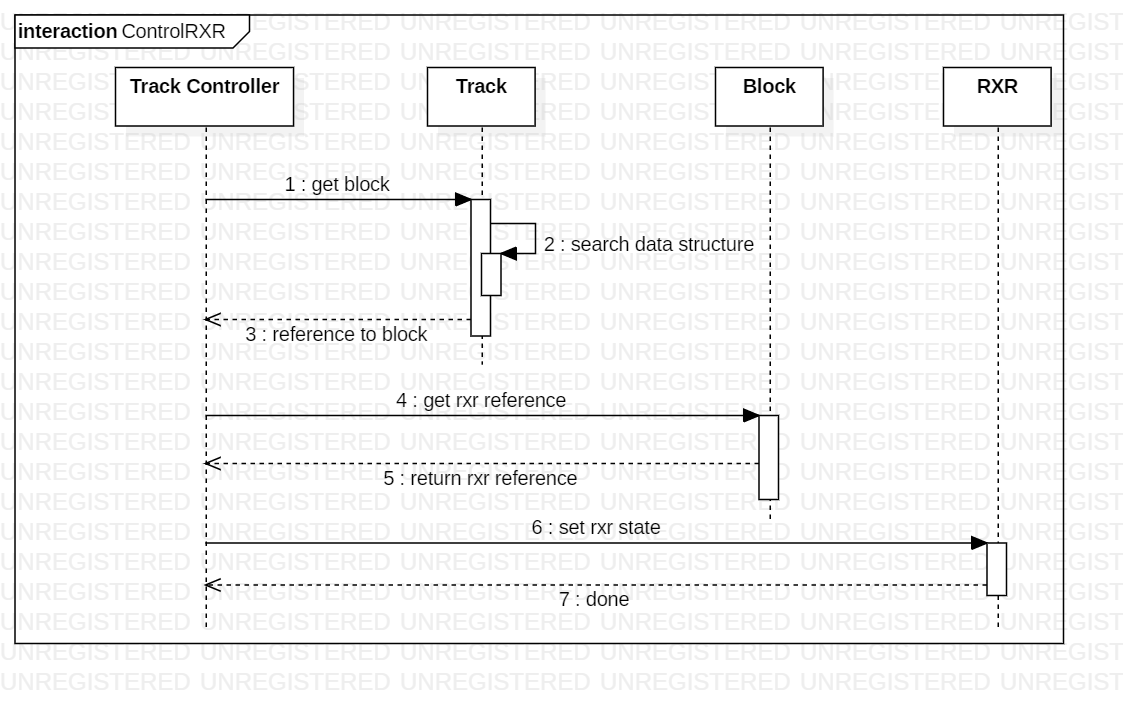
\includegraphics[width=\textwidth]{./SequenceDiagrams/TrackModel_SeqDiagrams/TrackModel_SeqDiagram_TKCControlsRXR.png}
        \caption{Use Case: Track Controller Controls Railroad Crossing State}
        \label{fig:Track Controller Controls RXR}
    \end{figure}
    \begin{figure}[H]
        \centering
        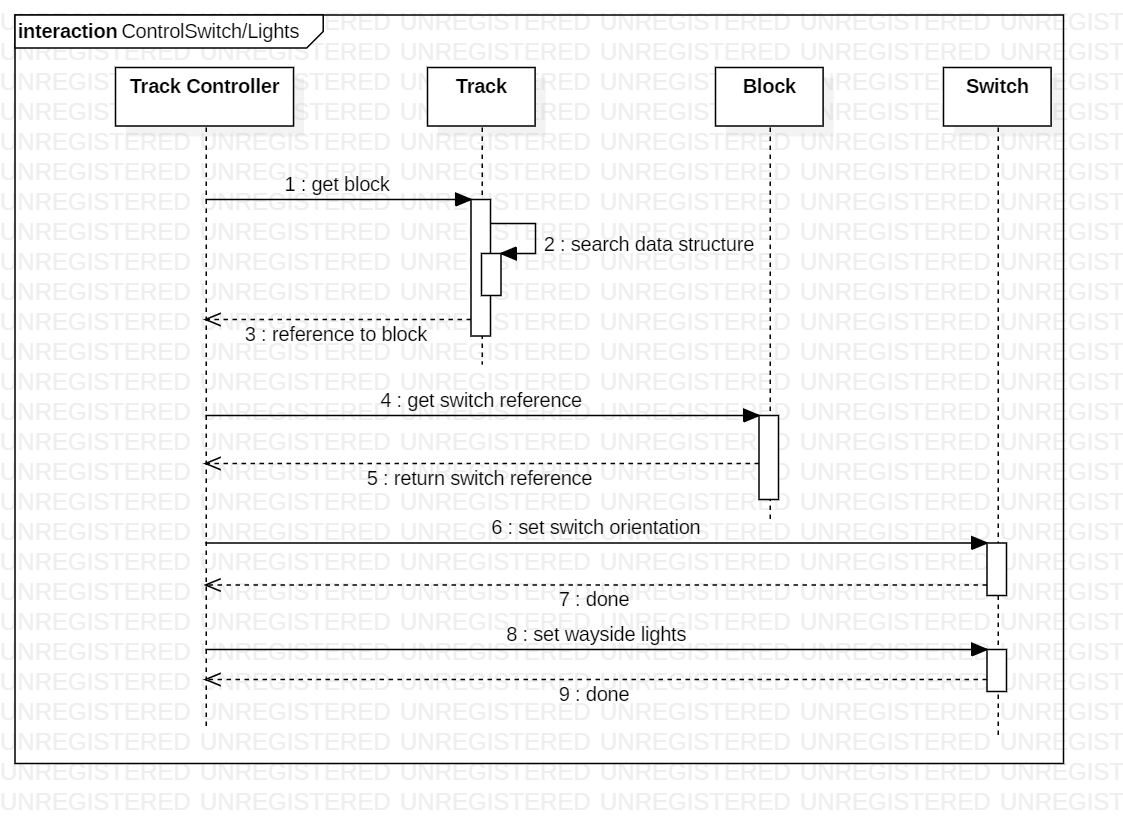
\includegraphics[width=\textwidth]{./SequenceDiagrams/TrackModel_SeqDiagrams/TrackModel_SeqDiagram_TKCControlsSwitch+Lights.png}
        \caption{Use Case: Track Controller Controls State of Switch and Wayside Lights}
        \label{fig: Track Controller Controls Switch and Lights}
    \end{figure}
    \begin{figure}[H]
        \centering
        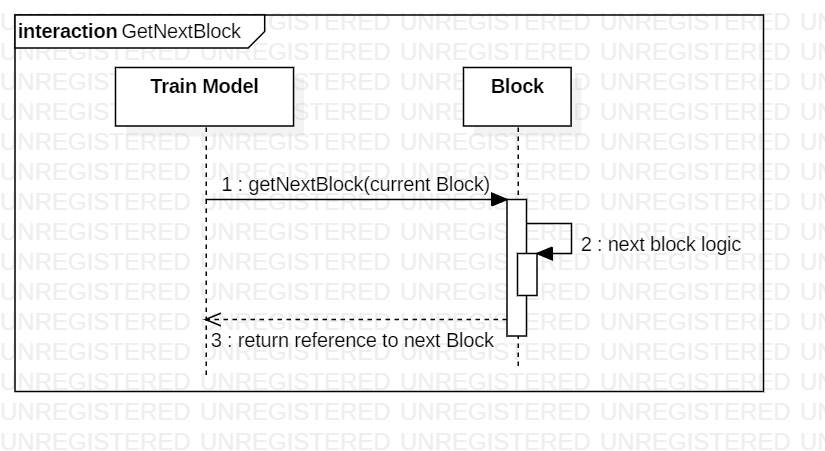
\includegraphics[width=\textwidth]{./SequenceDiagrams/TrackModel_SeqDiagrams/TrackModel_SeqDiagram_TNMGetNextBlock.png}
        \caption{Use Case: Train Model Requests Reference to Next Block in Path}
        \label{fig:Train Model Get Next Block}
    \end{figure}
    \begin{figure}[H]
        \centering
        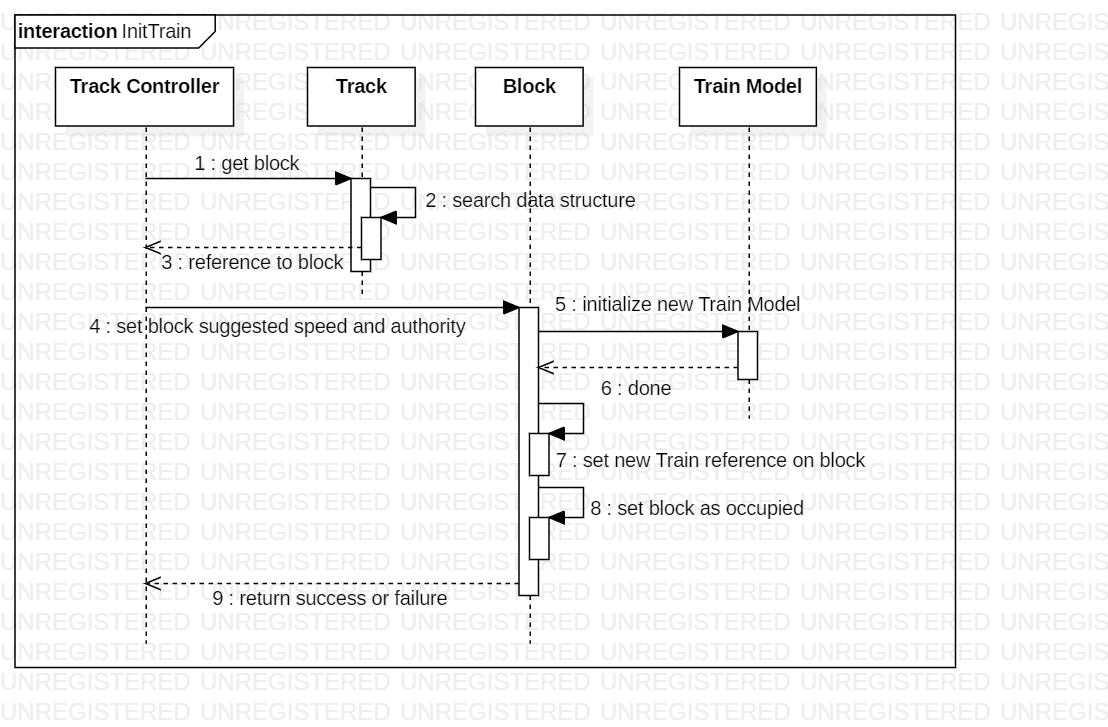
\includegraphics[width=\textwidth]{./SequenceDiagrams/TrackModel_SeqDiagrams/TrackModel_SeqDiagram_InitTrain.png}
        \caption{Use Case: Track Controller Initializes Train}
        \label{fig:Track Controller Initializes Train}
    \end{figure}
    \begin{figure}[H]
        \centering
        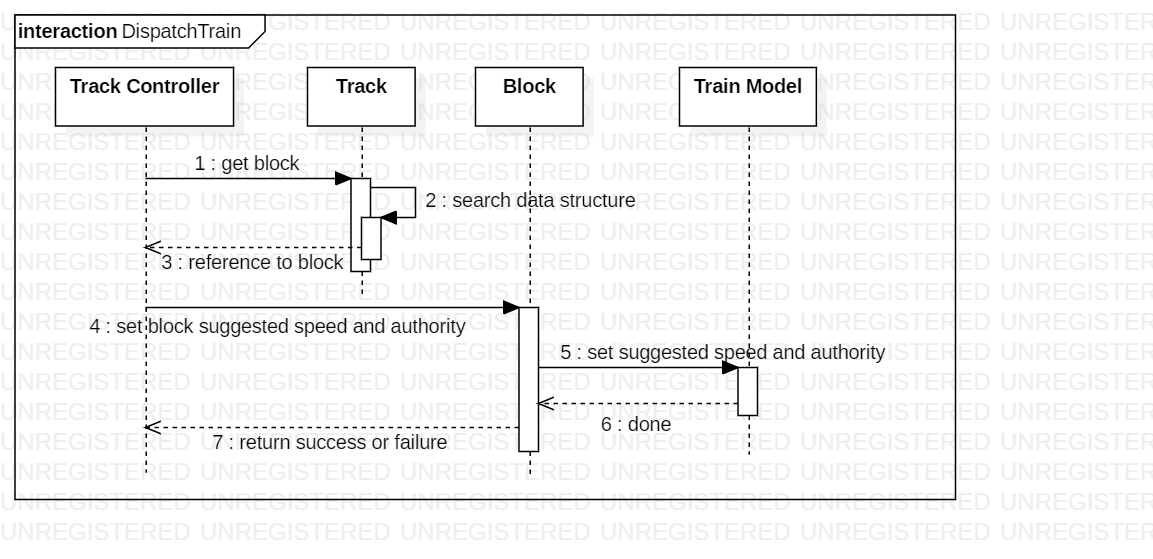
\includegraphics[width=\textwidth]{./SequenceDiagrams/TrackModel_SeqDiagrams/TrackModel_SeqDiagram_DispatchTrain.png}
        \caption{Use Case: Track Controller Dispatches Train}
        \label{fig:TrackSon}
    \end{figure}
    

    \subsection{Train Model}
    
    \subsubsection{Use Case Diagram}
    \begin{figure}[H]
        \centering
        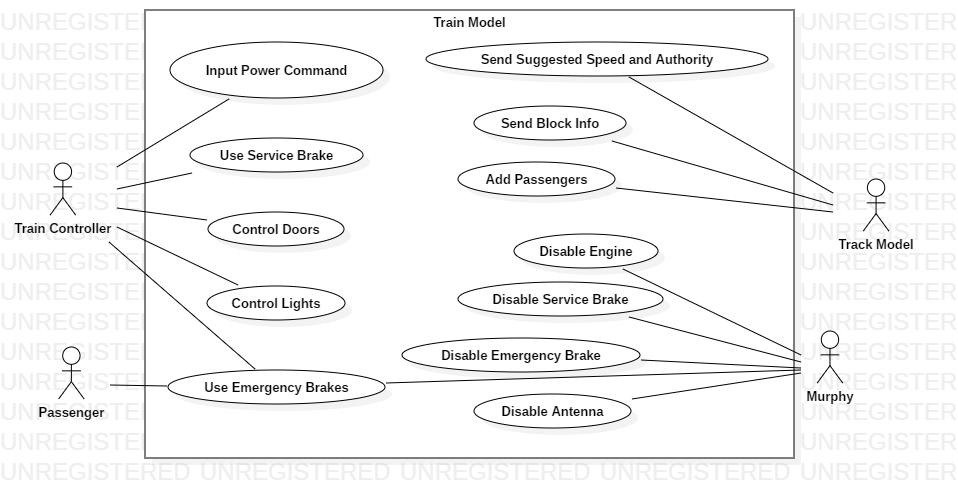
\includegraphics[width=\textwidth]{./TrainModel/TrainModel_UseCases.png}
        \caption{Train Model Use Cases}
        \label{fig:Train Model Use Cases}
    \end{figure}
    \subsubsection{Use Case Descriptions}
    \begin{longtable}{
    || >{\raggedright\arraybackslash}m{0.15 \textwidth}
    | >{\raggedright\arraybackslash}m{0.85 \textwidth}||}
    \hline
    \textbf{System} & \textbf{Train Model} \\
    \hline
    Use Case & Input a power command\\
    \hline
    Actors & Train Controller\\
    \hline
    Description & \begin{itemize}
        \item Train Controller inputs a power command
        \item The train calculates the current forces on it such as gravity
        \item The train calculates its new acceleration based on the power and forces
        \item The train calculates its new speed during the next system-wide update
    \end{itemize}\\
    \hline
    Data & Input: Power command \newline Output: forces, acceleration\\
    \hline
    Stimulus & Method call from Train Controller\\
    \hline
    Response & Force and acceleration values are updated\\
    \hline
    \end{longtable}
    
    \begin{longtable}{
    || >{\raggedright\arraybackslash}m{0.15 \textwidth}
    | >{\raggedright\arraybackslash}m{0.85 \textwidth}||}
    \hline
    \textbf{System} &  \textbf{Train Model} \\
    \hline
    Use Case & Train Controller activates service brake\\
    \hline
    Actors & Train Controller\\
    \hline
    Description & \begin{itemize}
        \item Train Controller activates the service brake
        \item The train decelerates at the max safe rate (see Blackpool specifications sheet)
        \item If brake remains on, train comes to a stop
    \end{itemize}\\
    \hline
    Data & Input: Service brake command \newline Output: acceleration\\
    \hline
    Stimulus & Method call from Train Controller\\
    \hline
    Response & Acceleration is changed, affecting speed on the next train update\\
    \hline
    \end{longtable}
    
    \begin{longtable}{
    || >{\raggedright\arraybackslash}m{0.15 \textwidth}
    | >{\raggedright\arraybackslash}m{0.85 \textwidth}||}
    \hline
    \textbf{System} &  \textbf{Train Model} \\
    \hline
    Use Case & Train Controller activates emergency brake\\
    \hline
    Actors & Train Controller\\
    \hline
    Description & \begin{itemize}
        \item Train Controller activates the emergency brake
        \item The train decelerates at the max safe rate (see Blackpool specifications sheet)
        \item If brake remains on, train comes to a stop
    \end{itemize}\\
    \hline
    Data & Input: Emergency brake command \newline Output: acceleration\\
    \hline
    Stimulus & Method call from Train Controller\\
    \hline
    Response & Acceleration is changed, affecting speed on the next train update\\
    \hline
    \end{longtable}
    
    \begin{longtable}{
    || >{\raggedright\arraybackslash}m{0.15 \textwidth}
    | >{\raggedright\arraybackslash}m{0.85 \textwidth}||}
    \hline
    \textbf{System} &  \textbf{Train Model} \\
    \hline
    Use Case & Train Controller sets the lights\\
    \hline
    Actors & Train Controller\\
    \hline
    Description & \begin{itemize}
        \item Train Controller calls a method to turn the lights on or off
        \item The train sets its lights field accordingly
    \end{itemize}\\
    \hline
    Data & Input: Boolean light state \newline Output: light state\\
    \hline
    Stimulus & Method call from Train Controller\\
    \hline
    Response & Train Model lights field set to true or false\\
    \hline
    \end{longtable}
    
    \begin{longtable}{
    || >{\raggedright\arraybackslash}m{0.15 \textwidth}
    | >{\raggedright\arraybackslash}m{0.85 \textwidth}||}
    \hline
    \textbf{System} &  \textbf{Train Model} \\
    \hline
    Use Case & Train Controller opens or closes a door\\
    \hline
    Actors & Train Controller\\
    \hline
    Description & \begin{itemize}
        \item Train Controller inputs desired state for a certain door
        \item Train sets specified door to that state
    \end{itemize}\\
    \hline
    Data & Input: door and state \newline Output: state of that door updated\\
    \hline
    Stimulus & Method call from Train Controller\\
    \hline
    Response & Door is updated\\
    \hline
    \end{longtable}
    
    \begin{longtable}{
    || >{\raggedright\arraybackslash}m{0.15 \textwidth}
    | >{\raggedright\arraybackslash}m{0.85 \textwidth}||}
    \hline
    \textbf{System} &  \textbf{Train Model} \\
    \hline
    Use Case & Track Model sends Suggested Speed and Authority\\
    \hline
    Actors & Track Model\\
    \hline
    Description & \begin{itemize}
        \item Track Model inputs suggested speed and authority
        \item Train Model updates its local fields to send to the Train Controller
    \end{itemize}\\
    \hline
    Data & Input: suggested speed, authority\newline Output: suggested speed and authority fields updated and passed to Train Controller\\
    \hline
    Stimulus & Method call from Track Model\\
    \hline
    Response & Train Model holds and passes on new suggested speed and authority\\
    \hline
    \end{longtable}
    
    \begin{longtable}{
    || >{\raggedright\arraybackslash}m{0.15 \textwidth}
    | >{\raggedright\arraybackslash}m{0.85 \textwidth}||}
    \hline
    \textbf{System} &  \textbf{Train Model} \\
    \hline
    Use Case & Train Model gets block info from Track Model\\
    \hline
    Actors & Track Model\\
    \hline
    Description & \begin{itemize}
        \item Train Model requests block info from the Track Model
        \item Track Model returns appropriate info
    \end{itemize}\\
    \hline
    Data & Input: Info request\newline Output: speed limit, grade, block length\\
    \hline
    Stimulus & Method call from Train Model\\
    \hline
    Response & Updated info on current block\\
    \hline
    \end{longtable}
    
    \begin{longtable}{
    || >{\raggedright\arraybackslash}m{0.15 \textwidth}
    | >{\raggedright\arraybackslash}m{0.85 \textwidth}||}
    \hline
    \textbf{System} &  \textbf{Train Model} \\
    \hline
    Use Case & Train Model requests the next block\\
    \hline
    Actors & Track Model\\
    \hline
    Description & \begin{itemize}
        \item Train Model calculates that it has traveled over an entire block
        \item Train Model tells the Track Model it has entered the next block
        \item Track Model internally assigns train to the next block
        \item Track Model tells train it has been reassigned
        \item Train Model requests info on the new block (see previous use case)
    \end{itemize}\\
    \hline
    Data & Input: New block\newline Output: placed in new block and given information for it\\
    \hline
    Stimulus & Method call from Train Model\\
    \hline
    Response & Both Track Model and Train Model are appropriately updated\\
    \hline
    \end{longtable}
    
    \begin{longtable}{
    || >{\raggedright\arraybackslash}m{0.15 \textwidth}
    | >{\raggedright\arraybackslash}m{0.85 \textwidth}||}
    \hline
    \textbf{System} &  \textbf{Train Model} \\
    \hline
    Use Case & Track Model tells a train to update its passengers at a station\\
    \hline
    Actors & Track Model\\
    \hline
    Description & \begin{itemize}
        \item Train comes to a stop at a station
        \item Track Model tells train to remove some passengers (if any present)
        \item Train removes some passengers and tells the track how much free space it has
        \item Track adds a random number of passengers such that the train is not overfilled
        \item Train updates its mass field based on number of passengers
    \end{itemize}\\
    \hline
    Data & Input: train stop at station\newline Output: train passenger number, train mass\\
    \hline
    Stimulus & Method call from Track Model\\
    \hline
    Response & Train has updated passenger and mass fields\\
    \hline
    \end{longtable}
    
    \begin{longtable}{
    || >{\raggedright\arraybackslash}m{0.15 \textwidth}
    | >{\raggedright\arraybackslash}m{0.85 \textwidth}||}
    \hline
    \textbf{System} &  \textbf{Train Model} \\
    \hline
    Use Case & Murphy causes a failure\\
    \hline
    Actors & Murphy\\
    \hline
    Description & \begin{itemize}
        \item Murphy chooses a failure state to set (engine failure, service/emergency brake failure, antenna failure)
        \item Train Model updates the selected failure state and modifies its behavior accordingly
    \end{itemize}\\
    \hline
    Data & Input: failure state, Boolean\newline Output: updated fields in Train Model\\
    \hline
    Stimulus & Method call from Murphy\\
    \hline
    Response & Train sets specified failure state, potentially altering its behavior\\
    \hline
    \end{longtable}
    
    \subsubsection{Class Diagrams}
    \begin{figure}[H]
        \centering
        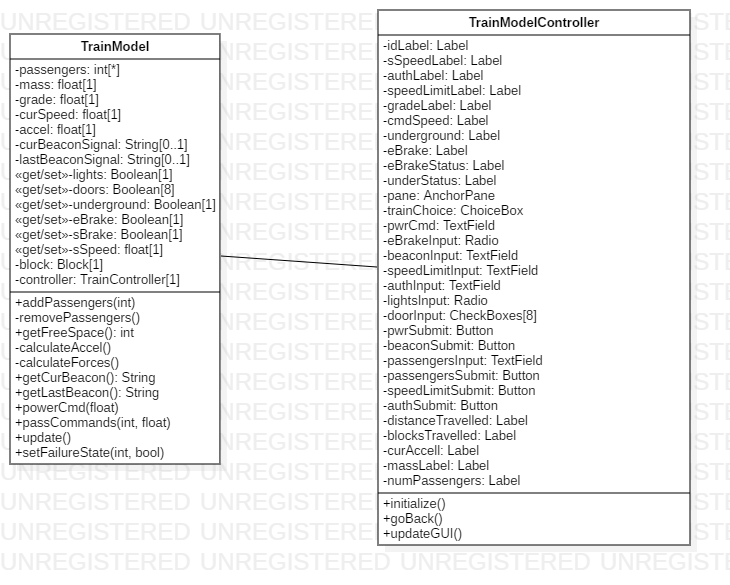
\includegraphics[width=\textwidth]{./TrainModel/TrainModel_ClassDiagram.png}
        \caption{Train Model Class Diagram}
        \label{fig:Train Model Class Diagram}
    \end{figure}
    
    \subsubsection{Sequence Diagrams}
    \begin{figure}[H]
        \centering
        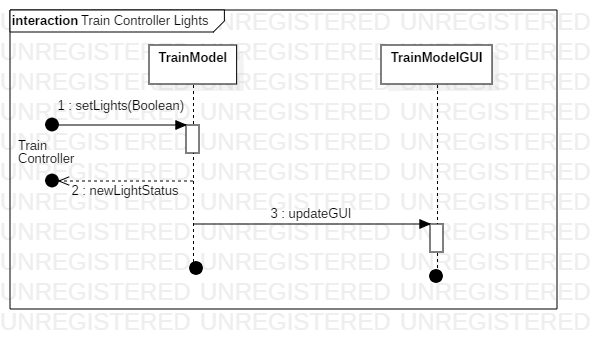
\includegraphics[width=\textwidth]{./TrainModel/ControlLights.png}
        \caption{Use Case: Train Controller sets Lights}
        \label{fig:Train Model Control Lights}
    \end{figure}
    \begin{figure}[H]
        \centering
        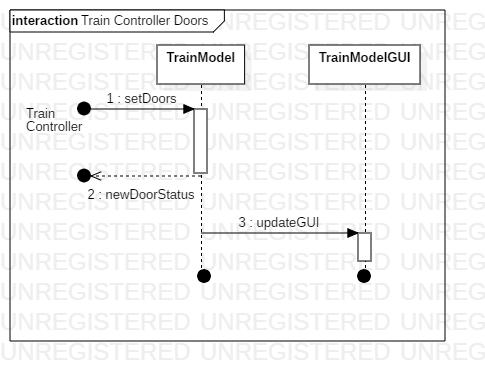
\includegraphics[width=\textwidth]{./TrainModel/Doors.png}
        \caption{Use Case: Train Controller sets Doors}
        \label{fig:Train Model Control Doors}
    \end{figure}
    \begin{figure}[H]
        \centering
        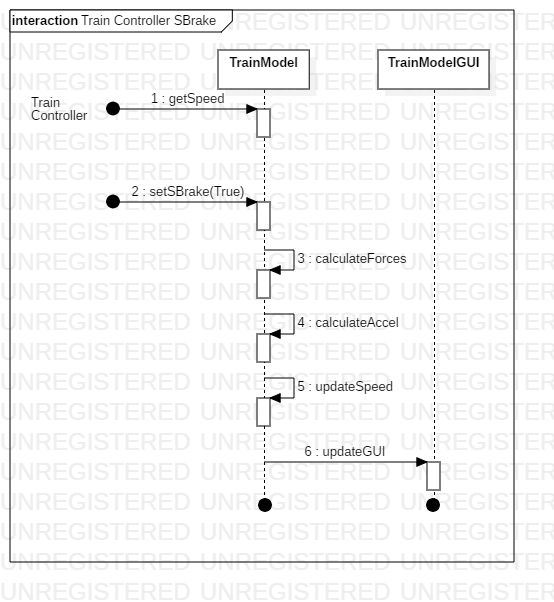
\includegraphics[width=\textwidth]{./TrainModel/SBrake.png}
        \caption{Use Case: Train Controller sets Service Brake}
        \label{fig:Train Model Service Brake}
    \end{figure}
    \begin{figure}[H]
        \centering
        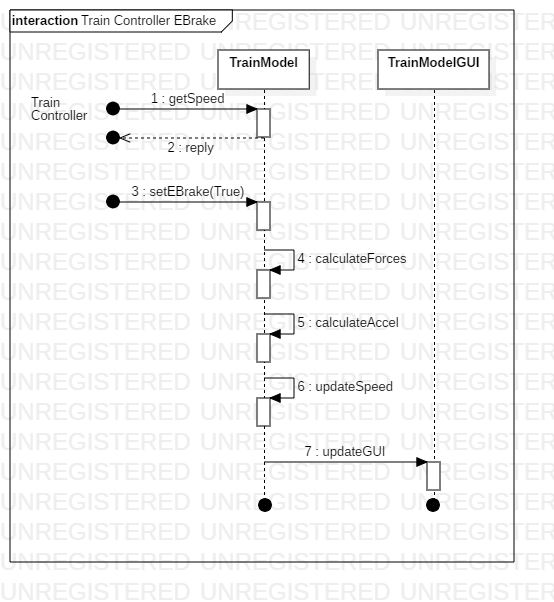
\includegraphics[width=\textwidth]{./TrainModel/EBrake.png}
        \caption{Use Case: Train Controller sets Emergency Brake}
        \label{fig:Train Model Emergency Brake}
    \end{figure}
    \begin{figure}[H]
        \centering
        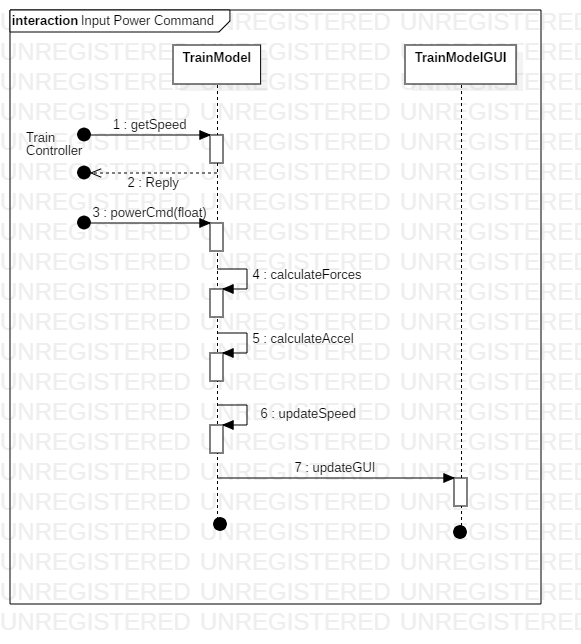
\includegraphics[width=\textwidth]{./TrainModel/PwrCmd.png}
        \caption{Use Case: Train Controller Gives Power Command}
        \label{fig:Train Model Power Command}
    \end{figure}
    \begin{figure}[H]
        \centering
        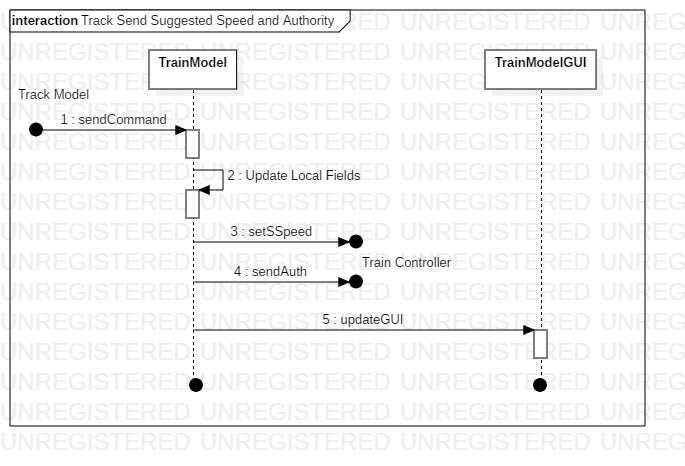
\includegraphics[width=\textwidth]{./TrainModel/SSpeedAuth.png}
        \caption{Use Case: Track Model Sends Suggested Speed and Authority}
        \label{fig:Train Model Speed Authority}
    \end{figure}
    \begin{figure}[H]
        \centering
        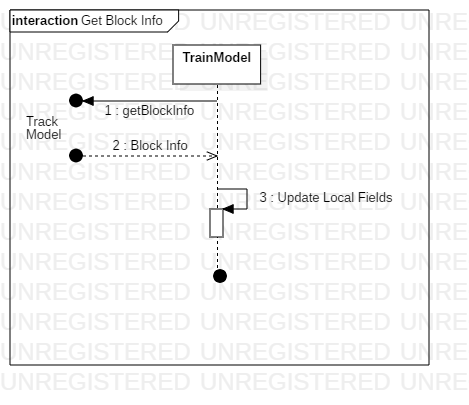
\includegraphics[width=\textwidth]{./TrainModel/GetBlockInfo.png}
        \caption{Use Case: Train Model gets Block Info from Track Model}
        \label{fig:Train Model Block Info}
    \end{figure}
    \begin{figure}[H]
        \centering
        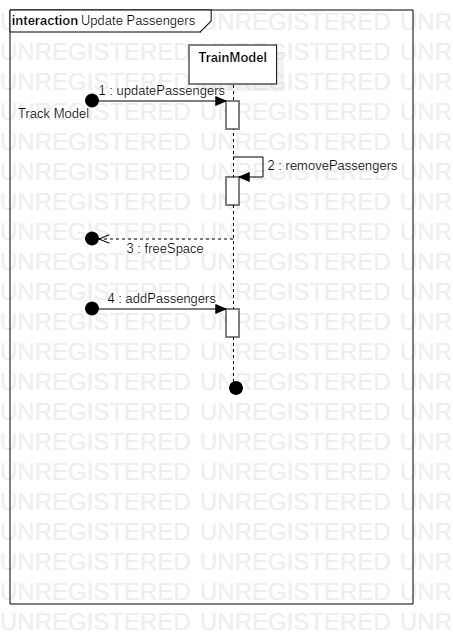
\includegraphics[width=\textwidth]{./TrainModel/UpdatePassengers.png}
        \caption{Use Case: Track Model tells Train Model to Update Passengers}
        \label{fig:Train Model Update Passengers}
    \end{figure}
    \begin{figure}[H]
        \centering
        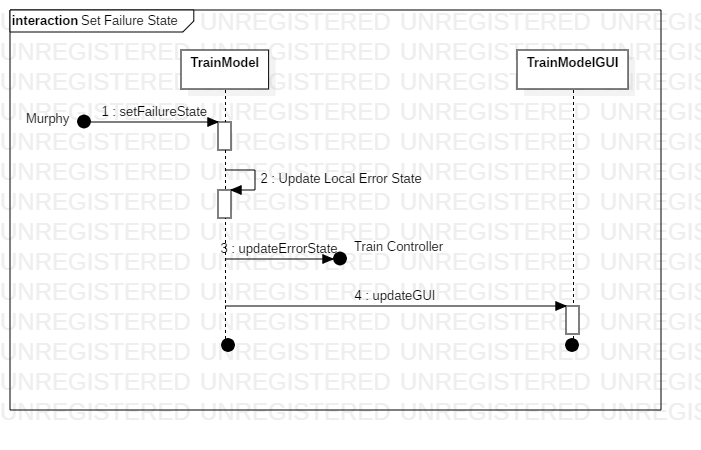
\includegraphics[width=\textwidth]{./TrainModel/SetFailureState.png}
        \caption{Use Case: Murphy sets a Failure State for the Train Model}
        \label{fig:Train Model Failure State}
    \end{figure}
    \begin{figure}[H]
        \centering
        \includegraphics[width=\textwidth]{./TrainModel/PassEBrake.png}
        \caption{Use Case: Passengers Activate Emergency Brake}
        \label{fig:Train Model Passenger Emergency Brake}
    \end{figure}
    \begin{figure}[H]
        \centering
        \includegraphics[width=\textwidth]{./TrainModel/Update.png}
        \caption{Use Case: Train Model Updates Itself}
        \label{fig:Train Model Block Info}
    \end{figure}
    \begin{figure}[H]
        \centering
        \includegraphics[width=\textwidth]{./TrainModel/NextBlock.png}
        \caption{Use Case: Train Model gets Next Block from Track Model}
        \label{fig:Train Model Next Block}
    \end{figure}
    

    \subsection{Train Controller}
    \subsubsection{Use Case Diagram}
    \begin{figure}[H]
        \centering
        \includegraphics[width=\textwidth]{./UseCaseDiagrams/TNCUCD2.png}
        \caption{Train Controller Use Cases}
        \label{fig:Train Controler Use Cases}
    \end{figure}
    \subsubsection{Use Case Descriptions}
    \begin{longtable}{
    || >{\raggedright\arraybackslash}m{0.15 \textwidth}
    | >{\raggedright\arraybackslash}m{0.85 \textwidth}||}
    \hline
    \textbf{System} & \textbf{Train Controller} \\
    \hline
    Use Case & Observe State of the Train Controller\\
    \hline
    Actors & Train Driver/Murphy\\
    \hline
    Description & \begin{itemize}
        \item Train Controller collects current operation data
        \item Train Controller GUI accepts this data
        \item Train Controller GUI updates its view with the new information
    \end{itemize}\\
    \hline
    Data & Input: None \newline Output: \\
    \hline
    Stimulus & Display of Train Controller Graphic User Interface\\
    \hline
    Response & Current operating conditions presented to use\\
    \hline
    \end{longtable}
    
     \begin{longtable}{
    || >{\raggedright\arraybackslash}m{0.15 \textwidth}
    | >{\raggedright\arraybackslash}m{0.85 \textwidth}||}
    \hline
    \textbf{System} & \textbf{Train Controller} \\
    \hline
    Use Case & Adjust Set-point Speed\\
    \hline
    Actors & Train Driver/Murphy\\
    \hline
    Description & \begin{itemize}
        \item Actor inputs a new set-point speed
        \item If E-Brake is activated, E-Brake signal is transmitted
        \item Sub-case: Train is operating in automatic mode
        \begin{itemize}
            \item Set-point speed is ignored in the determination of the power command and brake command
        \end{itemize}
        \item Sub-Case: Train is operating in manual mode
        \begin{itemize}
            \item Set-point speed is compared to suggested speed, lower speed is used to determine power and brake command
        \end{itemize}
        \item If determined speed is lower than operating speed, S-Brake signal is transmitted
        \item If determined speed is higher than operating speed, Power command is transmitted
    \end{itemize}\\
    \hline
    Data & Input: Setpoint Speed \newline Output: Power/Brake Command to Train Model\\
    \hline
    Stimulus & Actor enters a new setpoint speed\\
    \hline
    Response & Power or Brake command is transmitted to Train Model\\
    \hline
    \end{longtable}
    
     \begin{longtable}{
    || >{\raggedright\arraybackslash}m{0.15 \textwidth}
    | >{\raggedright\arraybackslash}m{0.85 \textwidth}||}
    \hline
    \textbf{System} & \textbf{Train Controller} \\
    \hline
    Use Case & Swap operational Mode\\
    \hline
    Actors & Train Driver/Murphy\\
    \hline
    Description & \begin{itemize}
        \item Actor selects a new operational mode
        \item Sub-case: Actor selects Manual
        \begin{itemize}
            \item Train controller enters manual mode
            \item The Set-point speed of the train defaults to the suggested speed
            \item The train controller user interface allows the user to input a set point speed
            \item The train controller considers the set-point speed in deciding commands to the train model
        \end{itemize}
        \item Sub-Case: Actor selects Automatic
        \begin{itemize}
            \item Train Controller enters automatic mode
            \item The train controller user interface restricts the adjustment of the setpoint speed
            \item The train controller does not consider the setpoint speed in deciding commands to the train model
        \end{itemize}
    \end{itemize}\\
    \hline
    Data & Input: None \newline Output: None\\
    \hline
    Stimulus & Actor selects an operational mode from the Train Controller user interface\\
    \hline
    Response & Operational decisions of the train controller are adjusted appropriately\\
    \hline
    \end{longtable}
    
    \begin{longtable}{
    || >{\raggedright\arraybackslash}m{0.15 \textwidth}
    | >{\raggedright\arraybackslash}m{0.85 \textwidth}||}
    \hline
    \textbf{System} & \textbf{Train Controller} \\
    \hline
    Use Case & Engage and Disengage E-Break\\
    \hline
    Actors & Train Driver/Murphy/Passenger\\
    \hline
    Description & \begin{itemize}
        \item Actor manipulates the E-Brake Control from either automatic or manual mode
        \item Sub-Case: E-Brake is activated 
        \begin{itemize}
            \item The train controller transmits an E-Brake command to the train model
            \item The train controller sets the mode of operation to manual
            \item The manipulation of the operational mode is restricted while the E-Brake is activated
        \end{itemize}
        \item Sub-Case: E-Brake is deactivated
        \begin{itemize}
            \item The Train controller stops transmitting the E-Brake command to the train model
            \item The train controller begins normal operation in the operational mode that was present before the E-Brake signal was activate.
            \item Manipulation of the E-Brake is enabled
        \end{itemize}
        
    \end{itemize}\\
    \hline
    Data & Input: Setpoint Speed \newline Output: Power/Brake Command to Train Model\\
    \hline
    Stimulus & Actor enters a new setpoint speed\\
    \hline
    Response & Power or Brake command is transmitted to Train Model\\
    \hline
    \end{longtable}
    
    \begin{longtable}{
    || >{\raggedright\arraybackslash}m{0.15 \textwidth}
    | >{\raggedright\arraybackslash}m{0.85 \textwidth}||}
    \hline
    \textbf{System} & \textbf{Train Controller} \\
    \hline
    Use Case & Program Ki and Kp\\
    \hline
    Actors & Train Engineer\\
    \hline
    Description & \begin{itemize}
        \item Train Engineer enters the programming view from the main display
        \item The Train engineer enters the new Ki and Kp into the display
        \item The new constants are utilized through all the train controllers of the system
    \end{itemize}\\
    \hline
    Data & Input: Ki (Double) Kp (Double)\newline Output: None \\
    \hline
    Stimulus & Train Engineer enters programming view from the main display view\\
    \hline
    Response & Train Controller is programmed with new PID constants\\
    \hline
    \end{longtable}
    
    \begin{longtable}{
    || >{\raggedright\arraybackslash}m{0.15 \textwidth}
    | >{\raggedright\arraybackslash}m{0.85 \textwidth}||}
    \hline
    \textbf{System} & \textbf{Train Controller} \\
    \hline
    Use Case & Transmit Track Circuit Information\\
    \hline
    Actors & Train Model\\
    \hline
    Description & \begin{itemize}
        \item Train Model receives a suggested speed, authority, and beacon information from the track circuit
        \item Train model sends that information to the train controller
    \end{itemize}\\
    \hline
    Data & Input: Setpoint Speed \newline Output: Power/Brake Command to Train Model\\
    \hline
    Stimulus & Train model receives new suggested speed, authority, and beacon, from the track circuit\\
    \hline
    Response & Train controller commands to train model correctly respond to transmitted information \\
    \hline
    \end{longtable}
    
    \begin{longtable}{
    || >{\raggedright\arraybackslash}m{0.15 \textwidth}
    | >{\raggedright\arraybackslash}m{0.85 \textwidth}||}
    \hline
    \textbf{System} & \textbf{Train Controller} \\
    \hline
    Use Case & Receive Power Command From Train\\
    \hline
    Actors & Train Model\\
    \hline
    Description & \begin{itemize}
        \item Use case "Program Ki and Kp" must have already been done
        \item Do use case "Transmit Track Circuit Information"
        \item The Train Controller will determine a proper t
    \end{itemize}\\
    \hline
    Data & Input: None \newline Output: Power Command\\
    \hline
    Stimulus & Function Call to Train Controller\\
    \hline
    Response & Power or Brake command is transmitted to Train Model\\
    \hline
    \end{longtable}
    
    
    \subsubsection{Class Diagrams}
    \begin{figure}[H]
        \centering
        \includegraphics[width=\textwidth]{./ClassDiagrams/TNCCD.png}
        \caption{Train Controller Class Diagram}
        \label{fig:Train Controler Class Diagram}
    \end{figure}
    
    \subsubsection{Sequence Diagrams}
    \begin{figure}[H]
        \centering
        \includegraphics[width=\textwidth]{./TNCSD/TrainEngineerPrograms.png}
        \caption{Train Engineer Programs Ki and Kp}
        \label{fig:Train Engineer Programs Ki and Kp}
    \end{figure}
    
    \begin{figure}[H]
        \centering
        \includegraphics[width=\textwidth]{./TNCSD/TrackCircuitTransmit.png}
        \caption{Train Model Transmits Track Circuit Information}
        \label{fig:Train Model Transmits Track Circuit Information}
    \end{figure}
    
    \begin{figure}[H]
        \centering
        \includegraphics[width=\textwidth]{./TNCSD/TRNDriverActEBrake.png}
        \caption{Train Driver or Murphy activates E-Brake}
        \label{fig:Train Driver or Murphy activates E-Brake}
    \end{figure}
    
    \begin{figure}[H]
        \centering
        \includegraphics[width=\textwidth]{./TNCSD/TRNDRiverDeactEBrake.png}
        \caption{Train Driver or Murphy deactivates E-Brake}
        \label{fig:Train Driver or Murphy deactivates E-Brake}
    \end{figure}
    
    \begin{figure}[H]
        \centering
        \includegraphics[width=\textwidth]{./TNCSD/TrnModelAct.png}
        \caption{Train Model activates E-Brake}
        \label{fig:Train Model activates E-Brake}
    \end{figure}
    
    \begin{figure}[H]
        \centering
        \includegraphics[width=\textwidth]{./TNCSD/TrnModelDeact.png}
        \caption{Train Model deactivates E-Brake}
        \label{fig:Train Model deactivates E-Brake}
    \end{figure}
    
    \begin{figure}[H]
        \centering
        \includegraphics[width=\textwidth]{./TNCSD/FaultDetected.png}
        \caption{Train Controller is notified of a fault}
        \label{fig:Train Controller is notified of a fault}
    \end{figure}

\end{document}